\documentclass[11pt,a4paper]{report}
\usepackage{color}
\usepackage{ifthen}
\usepackage{ifpdf}
\usepackage[headings]{fullpage}
\usepackage{listings}
\lstset{language=Java,breaklines=true}
\ifpdf \usepackage[pdftex, pdfpagemode={UseOutlines},bookmarks,colorlinks,linkcolor={blue},plainpages=false,pdfpagelabels,citecolor={red},breaklinks=true]{hyperref}
  \usepackage[pdftex]{graphicx}
  \pdfcompresslevel=9
  \DeclareGraphicsRule{*}{mps}{*}{}
\else
  \usepackage[dvips]{graphicx}
\fi

\newcommand{\entityintro}[3]{%
  \hbox to \hsize{%
    \vbox{%
      \hbox to .2in{}%
    }%
    {\bf  #1}%
    \dotfill\pageref{#2}%
  }
  \makebox[\hsize]{%
    \parbox{.4in}{}%
    \parbox[l]{5in}{%
      \vspace{1mm}%
      #3%
      \vspace{1mm}%
    }%
  }%
}
\newcommand{\refdefined}[1]{
\expandafter\ifx\csname r@#1\endcsname\relax
\relax\else
{$($in \ref{#1}, page \pageref{#1}$)$}\fi}
\date{\today}
\chardef\textbackslash=`\\
\usepackage{pdfpages}
\usepackage[utf8]{inputenc}
\usepackage[T1]{fontenc}
\usepackage[german]{babel}
\usepackage{hyperref}
\hypersetup{
	pdftitle={Pflichtenheft},
	bookmarks=true,
}
\usepackage{csquotes}

\usepackage{fancyhdr}%<-------------to control headers and footers
\usepackage[a4paper,margin=1in,footskip=.25in]{geometry}
\fancyhf{}
\fancyfoot[C]{\thepage} %<----to get page number below text
\pagestyle{fancy} %<-------the page style itself

\usepackage{xcolor}
\usepackage{framed}
\definecolor{shadecolor}{RGB}{220,220,220}
\usepackage{float}


\title{Android GO! App - Pflichtenheft}
\author{Gruppe 3}
\date{11.06.17}

% define custom lists
\usepackage{enumitem}
\usepackage{lipsum}

\begin{document}

\begin{titlepage}
	\begin{center}
	{\scshape\LARGE \bfseries Entwurfsdokument \par}
	\vspace{1cm}
	{\scshape\Large Praktikum der Softwareentwicklung \\ Sommersemester 2017\par}
	\vspace{1.5cm}
	{\huge\bfseries Android GO! App\par}
	\vspace{2cm}
	{\Large\itshape - Gruppe 3 -\par}
	\vfill
	{\bfseries erstellt von:\par}
	Arsenii Dunaev \\
	Florian Kröger \\
	Tina Maria Strößner \\
	Volodymyr Shpylka \\	
	\vfill
	% Bottom of the page
	{\large 09.07.17 \par}	
	\end{center}
\end{titlepage}

\begin{abstract}
Die Android App GO! ist eine mobile Applikation, die speziell zur Organisation von Treffen (z. B. gemeinsames Essen im Café oder in der Mensa) entwickelt wird. Beim erfolgreichen gemeinsamen Losgehen wird der gemittelte GPS-Standort von Mitgliedern der Gruppe angezeigt.\\

Dieses Dokument erläutert den Entwurf des Systems auf der Grundlage des Pflichtenhefts.
\end{abstract}

\sloppy
\addtocontents{toc}{\protect\markboth{Contents}{Contents}}
\tableofcontents



% add something here

\section{Änderungen zum Pflichtenheft}

Es wurden im Entwurf folgende Änderungen gegenüber dem Pflichtenheft vorgenommen:
\begin{enumerate}
	\item \textbf{Produktdaten - Benutzer} \\
	Es werden in den Produktdaten zusätzlich eine (von Firebase automatisch generierte) InstanceID gespeichert, die es dem Server erlaubt, Daten an das Android-Gerät eines bestimmten Benutzers zu senden.
	\item \textbf{Detailansicht der GOs} \\
	Es ist jedem Mitglied einer Gruppen (unabhängig von Teilnahmestatus) möglich, die Detailansicht eines GOs aufzurufen. Um den Karten-Tab öffnen zu können, um die Standorte der anderen Teilnahmer zu verfolgen, gilt weiterhin, dass der Teilnahmestatus 'Bestätigt' oder 'Unterwegs' lauten muss.
\end{enumerate}

\newpage

\section{Architekturstil und Paketstruktur}

\subsection{Client}
Die Architektur der Client-Applikation orientiert sich am Model-View-ViewModel (MVVM) Muster. Dies wird auf Android-Systemen durch die, auch hier eingesetzten, Architecture Components unterstützt. Das untenstehende Paketdiagramm zeigt den groben Aufbau der Client-Applikation, welche Abhängigkeiten bestehen und welche Aufgaben jedes Paket übernimmt. Genauere erläuterungen hierzu finden sich in den darauffolgenden Abschnitten.

\begin{figure}[H]
	\centering
	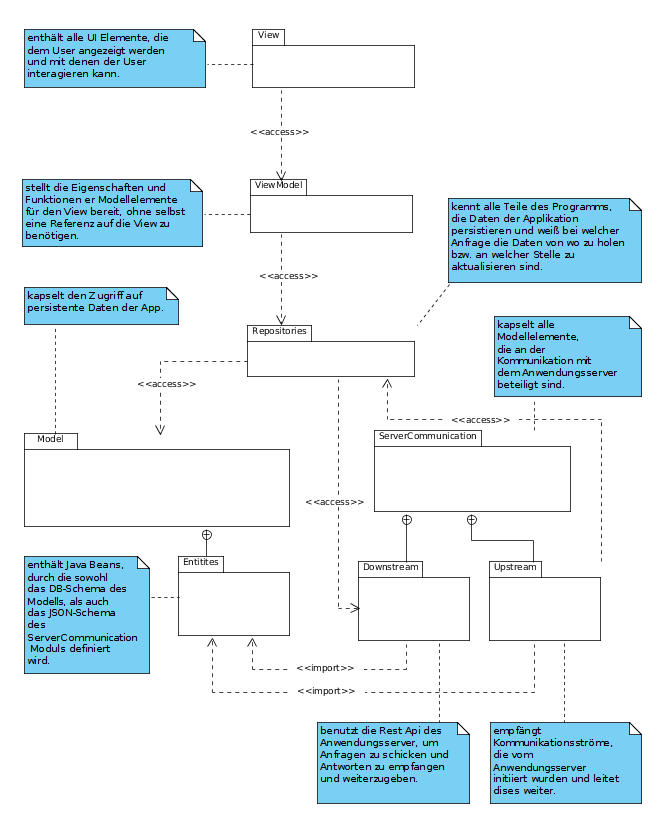
\includegraphics[scale=0.5]{../Klassendiagramme/paketdiagramm_client.png}
	\caption{Paketdiagramm der Clientanwendung}
\end{figure}

\subsubsection{Views}
Das Paket Views enthält alle Klassen, die am User Interface des Benutzers beteiligt sind. Das sind sämtliche Activities, Fragments und dazugehörige .xml-Layouts. Das Modul ist für die Präsentation der Appdaten sowie die Implementierung der Präsentationslogik (Umsetzung der Eigenschaften der Daten und Weiterleitung von Benutzereingaben) zuständig.

\textbf{Abhängigkeiten zu anderen Paketen:}\\
Das Paket Views kann die Informationen, die dem Benutzer angezeigt werden, nicht selbst generieren, sondern bekommt diese bereitgestellt von den entsprechenden ViewModells.

\textbf{Unterpakete:}\\
das Paket enthält das Unterpaket 'RecyclerView'. Da in der Applikation viele (verschiedene) RecyclerViews verwendet werden, gibt es für die Erstellung derselben ein eigenes Paket, dessen Aufgabe es ist, von den Datenobjekten die das Model liefert die gewünschten Informationen zu extrahieren und diese mit dem richtigen Layout zusammenzuführen. Innerhalb des Pakets besteht eine Abhängigkeit derjenigen View-Klassen, die einen RecyclerView verwenden zu dem Unterpaket RecyclerViews. Das Unterpaket RecyclerViews selbst ist nocht von anderen Klassen und Paketen abhängig.

\subsubsection{Modell}
Das Modell ist die Datenzugriffsschicht der Applikation, d.h. sie kapselt den Zugriff auf persistente Daten, die in einer lokalen SQLite Datenbank gehalten werden.Darüber hinaus enthält das Paket die Geschäftslogik der App, das hei?t hier werden die om ViewModel aufbereiteten und weitergeleiteten Befehle umgesetzt und anschließend die sich ergebenden Datenänderungen an das ViewModell zurückgegeben. Die Modellklassen, die sich lokal in der Applikation befinden, werden erweitert durch das Datenmodell, welches sich auf dem Server befindet. Es muss stets die Datenkonsistenz dieser zwei Modellteile sichergestellt werden (vgl. Paket Repository).

\textbf{Abhängigkeiten zu anderen Paketen}\\
Der Aufbau und die Operationen, die auf der lokalen Datenbank durchgeführt werden, werden mittels des Frameworks \textit{Room} realisiert.

\textbf{Unterpakete:}\\
Das Modell enthält das Unterpaket 'Entities'. Dies enthält die Java Entitäten, die von Room zu den Relationen der Datenbank umgesetzt werden. Die Datenbank kann von Room auch ohne eine Implementierung der Zugriffslogik aufgebaut werden. Die Entities haben demnach keine Anhängigkeiten zu anderen Klassen innerhalb des Programms. DIe Zugriffslogik der DAOs setzt hingegen die Existenz der Datenbank voraus, es gibt eine Abhängigkeit vom Modell zu den Entities.

\subsubsection{ViewModell}
Das ViewModell ist das Bindeglied zwischen View und Modell. Es tauscht Informationen mit dem Modell aus und stellt so der View öffentliche Eigenschaften und Befehle zur Verfügung, die an die Steuerungselemente der UI angebunden werden können. Dabei hat as ViewModell keine Referenz auf die View. Durch diese lose Kopplung kann die View jederzeit ausgetauscht werden, ohne dass das ViewModell verändert werden muss.

\textbf{Abhängigkeiten zu anderen Paketen}\\
Das ViewModell benötigt eine Referenz zum Modell, um die von der View empfangenen Befehle weiterleiten und die richtigen Daten von Modell anfordern zu können. Um diese Abhängigkeit zu entkoppeln und das Ansprechen der richtigen Modellkomponente zu erleichtern, wird diese Abhängigkeit über einen Vermittler ("Repository") geleitet. Dies ermöglicht das einfache Austauschen des Modells, ohne dass das ViewModell verändert werden muss.

\subsubsection{ServerCommunication}
Das Paket ServerCommunication übernimmt die Kommunikation der App mit dem Server, also das Speichern von Daten auf dem Server bzw. das Holen von Daten von dem Server. Darüber hinaus werden in diesem Paket auch Nachrichten, die vom Server gesendet werden empfangen und an das Modell zur Verarbeitung weitergeleitet.

\textbf{Abhängigkeiten zu anderen Paketen}\\
Das Paket hat keine Abhängigkeiten zu anderen Paketen der Applikation. Die Implementierung des REST-Clients erfolgt über das Framework \textit{Retrofit 2}. Hier besteht also eine Abhängigkeit zu einem externen Framework. Außerdem benötigt das Modukl zur fehlerfreien Ausführung seiner Aufgaben ein funktionierendes Backend (REST-Api, das die entsprechenden Ressourcen bereitstellt) des Systems.

\textbf{Unterpakete:}\\
Das Modul ServerCommunication setzt sich aus zwei Untermodulen zusammen. Das Modul \textit{Upstream} implementiert die Kommunikation, die über die REST-Api des Tomcat-Servers läuft, also jegliche Kommunikation, die von einem Client initiiert wird. Das Modul \textit{Downstream} hingegen ist dafür zuständig Kommunikationsströme zu empfangen, die vom Server initiiert werden und diese den Vermittlern zur Verbreitung weiterzuleiten.

\subsubsection{Repositories}
Wie in den vorherigen Abschnitten erläutert, ist die Geschäftslogik der App aufgeteilt auf den lokalen Teil (Modell) und einen Remote-Teil (ServerCommunication), die miteinander synchronisiert werden müssen. Zusätzlich müssen die ViewModells nach sämtlichen Änderungen mit den aktuellsten Daten versorgt werden. Dise Abhängigkeiten der einzelnen Komponenten werden in den Repository-Klassen zusammengefasst. Genauere Erläuterungen zur Funktionsweise finden sich in Abschnitt \ref{Vermittler}.

\textbf{Abhängigkeiten zu anderen Paketen:}\\
...

\subsection{Server}
Die Architektur ser Servers orientiert sich an einer MVC-Architektur. Das Programm des Servers ist in folgende Pakete aufgeteilt:
\begin{itemize}
	\item CommunicationLayer
	\item BusinessLayer
	\item PersistenceLayer
\end{itemize}

\subsubsection{CommunicationLayer}
Dieses Paket übernimmt die Rolle des Views. Die CommunicationLayer vereint alle Klassen, die an der Kommunication mit den Clients beteiligt sind. Es besteht aus den Unterpaketn Upstream und Downstream. Die Klassen des Pakets Upstream sind dafür zuständig, ein REST-API zur Verfügung zu stellen und auf Anfragen der Clients zu antworten, d.h. die Kommunikation wird von den Clients initiiert. Das Downstream-Paket hingegen schickt Nachrichten an Clients, ohne vorher von diesen angesprochen worden zu sein. Hierf"ur wird der Firebase Cloud Messaging Service benutzt.

\subsubsection{BusinessLayer}
Die BusinessLayer ist der Controller der Serveranwendung. dieses Modul realisiert Datenänderungen und Operationen auf der PersistenceLayer. Außerdem ist hier die Logik für die Erfassung und Auswertung der Standortdaten implementiert. Dies funktioniert ohne die Beteiligung des Modells, da diese Daten nur kurzfristig erfasst, verarbeitet und zurückgesendet werden müssen.

\subsubsection{PersistenceLayer}
Die PersistenceLayer bildet das Datenmodell. Sie ist für die Speicherung der Daten zuständig, sowie für die Weiterleitung an die Communicationlayer und somit an die Clients. Die PersistenceLayer setzt sich zusammen aus einer MySQL-Datenbank, die mit dem ORM-Framework Hibernate verwaltet wird und DAO-Klassen, in denen die Datenbankzugriffe gekapselt werden.

\newpage


\section{verwendete Entwurfsmuster}

\subsection{Schablonenmethode für SignInHelper}
Die verschiedenen Anmelde-Aktivitäten aller Loginhelper-Klassen können über die signIn()-Methode angesto"sen werden. Der spezifische Ablauf der Anmelde-Aktivität wird in den Unterklassen durch die primitiven Methoden definiert. \\

\textbf{beteiligte Klassen:}
\begin{itemize}
	\item SignInHelper: besitzt die Methode signIn(), die als Schablonenmethode dient und bei der Ausführung die primitiven Methoden configureSignIn() und startSignInProcess() aufruft
	\item FirebaseSignInHelper: Unterklasse von SignInHelper, die die primitiven Methoden configureSignIn() und startSignInProcess() implementiert
	\item GoSignInHelper: Unterklasse von SignInHelper, die die primitiven Methoden configureSignIn() und startSignInProcess() implementiert
\end{itemize}

\subsection{Beobachter zum Aktualisieren des UI}
Durch das Ausführen von Befehlen von einem Benutzer, kann es zu Änderngen in den Daten kommen, die eine Änderung des aktuellen Views anderer Benutzer erfordern. Diese 1-zu-n Abhängigkeit wird durch ein Beobachter-muster behandelt. Die dafür benötigte Funktionalität wird von der Architecture-Components Framework Klasse LiveData<> bereitgestellt. Ein Objekt dieser Klasse kann von einem LifeCycleOwner (z.B. eine Lifecycle-Activity oder ein LifecycleFragment) beobachtet werden und löst bei Änderung den Methodenaufruf \textit{onChanged()} aus. Die Livedata-Objekte sind Lifecycle-Aware, das bedeutet eine Benachrichtigung über eine Änderung wird nur dann an einen Beobachter weitergeleitet, wenn er sich in einem aktiven Stadium seines Lifecycles befindet.\\
\textbf{beteiligte Klassen:}
\begin{itemize}
	\item \textit{LiveData<>:}\\ das beobachtete Subjekt
	\item \textit{BaseActivity (die von LifecycleActivity erbt):}\\ Der Beobachter, der bei Änderung der Daten benachrichtigt wird und daraufhin das dem Benutzer präsentierte UI aktualisiert.
\end{itemize}

\subsection{DAO-Pattern zur lokalen Persisitierung von Daten}
Damit nicht bei jeder Datenanforderung, die vom UI gestellt wird, ein Zugriff auf den Tomcat-Server unternommen werden muss, werden die Daten des Benutzers lokal in einer SQLite Datenbank persistiert. Die Implementierung des Datenbankschemas und der Datenbankzugriffe wird mithilfe des Android-Framworks Room realisiert. Dabei wird ein Data Access Object Pattern verwendet.
Die Entity-Beans definieren dabei, wie das Schema der Datenbank aufgebaut wird (jede als entity annotierte klasse wird als eine Tabelle in der Datenbank umgesetzt), die DAO-Interfaces definieren die Methoden, mit denen vom Programm aus af die Datenbank zugegriffen werden kann.\\

\textbf{beteiligte Klassen:}
\begin{itemize}
	\item \textit{User, Go, Group:}\\ Entity-Beans, die die Struktur der Datenbankrelationen darstellen
	\item \textit{UserDao, GoDao, GroupDao:}\\ Data-Access-Object Interfaces, die die eigentlichen Zugriffe auf die Datenbank übernehmen.
\end{itemize}

\subsection{Vermittler zur Koordination von Datenzugriffen}\label{Vermittler}
Wenn der Benutzer bestimmte Daten anzigen will, muss die App diese Daten zunächst beschaffen, entweder aus den lokal persisitierten Daten oder gegebenenfalls vom Remote-Server des Systems- Ähnlich verhält es sich mit Änderungen von Daten: Die Änderungen müssen sowohl lokal in der SQLIte Datenbank und im ViewModell, als auch auch der zentralen Datenbank des Server geändert werden.\\
Um diese vielen Abhängigkeiten zu verwalten und die Konsistenz der Daten sicherzustellen, sollen Datarepository-Klasssen implementiert werden, die als Vermittler zwischen den Kollegen dienen.
So muss das ViewModell zum Erstellen/Ändern/Löschen von Daten lediglich das DataRepository ansprechen, ohne die darunterliegende Datenpersistenzlogik zu kennen. Auch der Server kommuniziert seine Daten nur mit der Datarepository. Modell und Viewmodell müssen sich so gegenseitig nicht referenzieren, sondern für alle Komponenten eyisitert ein zentraler Ansprechpartner.\\

\textbf{beteiligte Klassen:}
\begin{itemize}
	\item \textit{GoRepository/GroupRepository:}\\
	 Vermittler
	\item \textit{ViewModell, TomcatrestApi, Dao:}\\ Kollegen
\end{itemize}

\subsection{DAO Pattern für Datenpersistenz auf dem Server}

\subsection{Strategiemuster zur Kapselung des Clustering-Alogithmus}
Das Clustern der Standorte der Teilnehmer eines GOs wird von der Klasse GoClusterStrategy übernommen. Diese Klasse ist mittels eines Strategy-Patterns in das Programm eingebunden. Dies entkoppelt den Algorithmus von seinem Kontext und erkann dynamisch durch andere Clustering-Alogirthmen ersetzt oder ergänzt werden. \\

\textbf{beteiligte Klassen:}
\begin{itemize}
	\item \textit{LocationService} \\
	Die Klasse ist der Kontext der Clustering-Strategie. Von hier aus wird die Ausführung des Algorithmus angestoßen.
	\item \textit{ClusterStrategy} \\
	ClusterStrategy ist ein Interface, das von jedem Cluster-Algorithmus implementiert werden muss. Es definiert eine \textit{caluculateCluster()} Methode, die eine Liste an einzelnen User-Standorten entgegen nimmt und eine Liste an User-Clustern zurückgibt.
	\item \textit{GoClusterStrategy} \\
	In dieser Klasse wird der Clustering-Algorithmus implementiert, der angewendet werden soll. Die Klasse erweitert das Interface ClusterStrategy.
\end{itemize}

\subsection{Fassade zur Vereinfachung des Server Interfaces}
Der verwendete Tomcat-Server bietet seinem Clients zur Kommunikation ein REST Interface an. Das Ansprechen der verschiedenen REST Ressourcen ist in der App hinter dem Interface \textit{TomcatRestApi}. Das Interface bietet den aufrufenden Klassen Methoden zum aufrufen der REST Ressourcen an, ohne das ein Aufrufer etwas von der eigentlichen Kommunikation mit dem Server wissen muss. \\

\textbf{beteiligte Klassen}
\begin{itemize}
	\item \textit{TomcatRestApi} \\
	Das Interface ist die Fassade, die die Schnittstelle zum Tomcat-Server hinter sich versteckt. Nach außen werden Methoden bereitgestellt, die von anderen Klassen aufgerufen werden können, um Server-Dienste in Anspruch nehmen zu können, ohne sich um die Details der Kommunikation zu kümmern.
\end{itemize}

\section{Klassenbeschreibungen}

% ------- textdoclet_include/intro.tex end

\section*{Class Hierarchy}{
\thispagestyle{empty}
\markboth{Class Hierarchy}{Class Hierarchy}
\addcontentsline{toc}{section}{Class Hierarchy}
\subsection*{Classes}
{\raggedright
\hspace{0.0cm} $\bullet$ java.lang.Object {\tiny \refdefined{java.lang.Object}} \\
\hspace{1.0cm} $\bullet$  {\tiny } \\
\hspace{2.0cm} $\bullet$ edu.kit.pse17.go\_app.view.recyclerView.ListAdapter {\tiny \refdefined{edu.kit.pse17.go_app.view.recyclerView.ListAdapter}} \\
\hspace{1.0cm} $\bullet$ AppCompatActivity {\tiny } \\
\hspace{2.0cm} $\bullet$ edu.kit.pse17.go\_app.login.SignInHelper {\tiny \refdefined{edu.kit.pse17.go_app.login.SignInHelper}} \\
\hspace{3.0cm} $\bullet$ edu.kit.pse17.go\_app.login.FirebaseSignInHelper {\tiny \refdefined{edu.kit.pse17.go_app.login.FirebaseSignInHelper}} \\
\hspace{3.0cm} $\bullet$ edu.kit.pse17.go\_app.login.GoSignInHelper {\tiny \refdefined{edu.kit.pse17.go_app.login.GoSignInHelper}} \\
\hspace{1.0cm} $\bullet$ FirebaseInstanceIdService {\tiny } \\
\hspace{2.0cm} $\bullet$ edu.kit.pse17.go\_app.serverCommunication.downstream.TokenService {\tiny \refdefined{edu.kit.pse17.go_app.serverCommunication.downstream.TokenService}} \\
\hspace{1.0cm} $\bullet$ FirebaseMessagingService {\tiny } \\
\hspace{2.0cm} $\bullet$ edu.kit.pse17.go\_app.serverCommunication.downstream.MessagingService {\tiny \refdefined{edu.kit.pse17.go_app.serverCommunication.downstream.MessagingService}} \\
\hspace{1.0cm} $\bullet$ LifecycleActivity {\tiny } \\
\hspace{2.0cm} $\bullet$ edu.kit.pse17.go\_app.view.BaseActivity {\tiny \refdefined{edu.kit.pse17.go_app.view.BaseActivity}} \\
\hspace{3.0cm} $\bullet$ edu.kit.pse17.go\_app.view.GoDetailActivity {\tiny \refdefined{edu.kit.pse17.go_app.view.GoDetailActivity}} \\
\hspace{4.0cm} $\bullet$ edu.kit.pse17.go\_app.view.GoDetailActivityOwner {\tiny \refdefined{edu.kit.pse17.go_app.view.GoDetailActivityOwner}} \\
\hspace{3.0cm} $\bullet$ edu.kit.pse17.go\_app.view.GroupDetailActivity {\tiny \refdefined{edu.kit.pse17.go_app.view.GroupDetailActivity}} \\
\hspace{4.0cm} $\bullet$ edu.kit.pse17.go\_app.view.GroupDetailActivityAdmin {\tiny \refdefined{edu.kit.pse17.go_app.view.GroupDetailActivityAdmin}} \\
\hspace{3.0cm} $\bullet$ edu.kit.pse17.go\_app.view.GroupListActivity {\tiny \refdefined{edu.kit.pse17.go_app.view.GroupListActivity}} \\
\hspace{3.0cm} $\bullet$ edu.kit.pse17.go\_app.view.InformationActivity {\tiny \refdefined{edu.kit.pse17.go_app.view.InformationActivity}} \\
\hspace{3.0cm} $\bullet$ edu.kit.pse17.go\_app.view.SettingsActivity {\tiny \refdefined{edu.kit.pse17.go_app.view.SettingsActivity}} \\
\hspace{3.0cm} $\bullet$ edu.kit.pse17.go\_app.view.SignInActivity {\tiny \refdefined{edu.kit.pse17.go_app.view.SignInActivity}} \\
\hspace{1.0cm} $\bullet$ RoomDatabase {\tiny } \\
\hspace{2.0cm} $\bullet$ edu.kit.pse17.go\_app.model.LocalDatabase {\tiny \refdefined{edu.kit.pse17.go_app.model.LocalDatabase}} \\
\hspace{1.0cm} $\bullet$ ViewHolder {\tiny } \\
\hspace{2.0cm} $\bullet$ edu.kit.pse17.go\_app.view.recyclerView.ListViewHolder {\tiny \refdefined{edu.kit.pse17.go_app.view.recyclerView.ListViewHolder}} \\
\hspace{1.0cm} $\bullet$ ViewModel {\tiny } \\
\hspace{2.0cm} $\bullet$ edu.kit.pse17.go\_app.viewModel.GoListViewModel {\tiny \refdefined{edu.kit.pse17.go_app.viewModel.GoListViewModel}} \\
\hspace{2.0cm} $\bullet$ edu.kit.pse17.go\_app.viewModel.GoViewModel {\tiny \refdefined{edu.kit.pse17.go_app.viewModel.GoViewModel}} \\
\hspace{2.0cm} $\bullet$ edu.kit.pse17.go\_app.viewModel.GroupListViewModel {\tiny \refdefined{edu.kit.pse17.go_app.viewModel.GroupListViewModel}} \\
\hspace{2.0cm} $\bullet$ edu.kit.pse17.go\_app.viewModel.GroupViewModel {\tiny \refdefined{edu.kit.pse17.go_app.viewModel.GroupViewModel}} \\
\hspace{2.0cm} $\bullet$ edu.kit.pse17.go\_app.viewModel.LocationViewModel {\tiny \refdefined{edu.kit.pse17.go_app.viewModel.LocationViewModel}} \\
\hspace{1.0cm} $\bullet$ edu.kit.pse17.go\_app.ClientCommunication.Downstream.FcmClient {\tiny \refdefined{edu.kit.pse17.go_app.ClientCommunication.Downstream.FcmClient}} \\
\hspace{1.0cm} $\bullet$ edu.kit.pse17.go\_app.ClientCommunication.Upstream.GroupRestController {\tiny \refdefined{edu.kit.pse17.go_app.ClientCommunication.Upstream.GroupRestController}} \\
\hspace{1.0cm} $\bullet$ edu.kit.pse17.go\_app.ClientCommunication.Upstream.UserRestController {\tiny \refdefined{edu.kit.pse17.go_app.ClientCommunication.Upstream.UserRestController}} \\
\hspace{1.0cm} $\bullet$ edu.kit.pse17.go\_app.Main {\tiny \refdefined{edu.kit.pse17.go_app.Main}} \\
\hspace{1.0cm} $\bullet$ edu.kit.pse17.go\_app.PersistenceLayer.GoEntity {\tiny \refdefined{edu.kit.pse17.go_app.PersistenceLayer.GoEntity}} \\
\hspace{1.0cm} $\bullet$ edu.kit.pse17.go\_app.PersistenceLayer.GroupEntity {\tiny \refdefined{edu.kit.pse17.go_app.PersistenceLayer.GroupEntity}} \\
\hspace{1.0cm} $\bullet$ edu.kit.pse17.go\_app.PersistenceLayer.UserEntity {\tiny \refdefined{edu.kit.pse17.go_app.PersistenceLayer.UserEntity}} \\
\hspace{1.0cm} $\bullet$ edu.kit.pse17.go\_app.PersistenceLayer.daos.AbstractDao {\tiny \refdefined{edu.kit.pse17.go_app.PersistenceLayer.daos.AbstractDao}} \\
\hspace{2.0cm} $\bullet$ edu.kit.pse17.go\_app.PersistenceLayer.daos.GoDaoImp {\tiny \refdefined{edu.kit.pse17.go_app.PersistenceLayer.daos.GoDaoImp}} \\
\hspace{2.0cm} $\bullet$ edu.kit.pse17.go\_app.PersistenceLayer.daos.GroupDaoImp {\tiny \refdefined{edu.kit.pse17.go_app.PersistenceLayer.daos.GroupDaoImp}} \\
\hspace{2.0cm} $\bullet$ edu.kit.pse17.go\_app.PersistenceLayer.daos.UserDaoImp {\tiny \refdefined{edu.kit.pse17.go_app.PersistenceLayer.daos.UserDaoImp}} \\
\hspace{1.0cm} $\bullet$ edu.kit.pse17.go\_app.PersistenceLayer.daos.GoDaoImp.GoEventArg {\tiny \refdefined{edu.kit.pse17.go_app.PersistenceLayer.daos.GoDaoImp.GoEventArg}} \\
\hspace{1.0cm} $\bullet$ edu.kit.pse17.go\_app.ServiceLayer.GoClusterStrategy {\tiny \refdefined{edu.kit.pse17.go_app.ServiceLayer.GoClusterStrategy}} \\
\hspace{1.0cm} $\bullet$ edu.kit.pse17.go\_app.ServiceLayer.GoService {\tiny \refdefined{edu.kit.pse17.go_app.ServiceLayer.GoService}} \\
\hspace{1.0cm} $\bullet$ edu.kit.pse17.go\_app.ServiceLayer.GroupService {\tiny \refdefined{edu.kit.pse17.go_app.ServiceLayer.GroupService}} \\
\hspace{1.0cm} $\bullet$ edu.kit.pse17.go\_app.ServiceLayer.LocationService {\tiny \refdefined{edu.kit.pse17.go_app.ServiceLayer.LocationService}} \\
\hspace{1.0cm} $\bullet$ edu.kit.pse17.go\_app.ServiceLayer.LocationService.Cluster {\tiny \refdefined{edu.kit.pse17.go_app.ServiceLayer.LocationService.Cluster}} \\
\hspace{1.0cm} $\bullet$ edu.kit.pse17.go\_app.ServiceLayer.LocationService.UserLocation {\tiny \refdefined{edu.kit.pse17.go_app.ServiceLayer.LocationService.UserLocation}} \\
\hspace{1.0cm} $\bullet$ edu.kit.pse17.go\_app.ServiceLayer.Observer {\tiny \refdefined{edu.kit.pse17.go_app.ServiceLayer.Observer}} \\
\hspace{1.0cm} $\bullet$ edu.kit.pse17.go\_app.ServiceLayer.UserService {\tiny \refdefined{edu.kit.pse17.go_app.ServiceLayer.UserService}} \\
\hspace{1.0cm} $\bullet$ edu.kit.pse17.go\_app.model.entities.Cluster {\tiny \refdefined{edu.kit.pse17.go_app.model.entities.Cluster}} \\
\hspace{1.0cm} $\bullet$ edu.kit.pse17.go\_app.model.entities.Go {\tiny \refdefined{edu.kit.pse17.go_app.model.entities.Go}} \\
\hspace{1.0cm} $\bullet$ edu.kit.pse17.go\_app.model.entities.Group {\tiny \refdefined{edu.kit.pse17.go_app.model.entities.Group}} \\
\hspace{1.0cm} $\bullet$ edu.kit.pse17.go\_app.model.entities.GroupMembership {\tiny \refdefined{edu.kit.pse17.go_app.model.entities.GroupMembership}} \\
\hspace{1.0cm} $\bullet$ edu.kit.pse17.go\_app.model.entities.User {\tiny \refdefined{edu.kit.pse17.go_app.model.entities.User}} \\
\hspace{1.0cm} $\bullet$ edu.kit.pse17.go\_app.model.entities.UserGoStatus {\tiny \refdefined{edu.kit.pse17.go_app.model.entities.UserGoStatus}} \\
\hspace{1.0cm} $\bullet$ edu.kit.pse17.go\_app.repositories.GoRepository {\tiny \refdefined{edu.kit.pse17.go_app.repositories.GoRepository}} \\
\hspace{1.0cm} $\bullet$ edu.kit.pse17.go\_app.repositories.GroupRepository {\tiny \refdefined{edu.kit.pse17.go_app.repositories.GroupRepository}} \\
\hspace{1.0cm} $\bullet$ edu.kit.pse17.go\_app.repositories.LocationRepository {\tiny \refdefined{edu.kit.pse17.go_app.repositories.LocationRepository}} \\
\hspace{1.0cm} $\bullet$ edu.kit.pse17.go\_app.serverCommunication.upstream.RestMessagingService {\tiny \refdefined{edu.kit.pse17.go_app.serverCommunication.upstream.RestMessagingService}} \\
\hspace{1.0cm} $\bullet$ edu.kit.pse17.go\_app.view.GoListActivity {\tiny \refdefined{edu.kit.pse17.go_app.view.GoListActivity}} \\
\hspace{1.0cm} $\bullet$ edu.kit.pse17.go\_app.view.recyclerView.listItems.GOListItem {\tiny \refdefined{edu.kit.pse17.go_app.view.recyclerView.listItems.GOListItem}} \\
\hspace{1.0cm} $\bullet$ edu.kit.pse17.go\_app.view.recyclerView.listItems.GroupListItem {\tiny \refdefined{edu.kit.pse17.go_app.view.recyclerView.listItems.GroupListItem}} \\
\hspace{1.0cm} $\bullet$ edu.kit.pse17.go\_app.view.recyclerView.listItems.UserMailListItem {\tiny \refdefined{edu.kit.pse17.go_app.view.recyclerView.listItems.UserMailListItem}} \\
\hspace{1.0cm} $\bullet$ edu.kit.pse17.go\_app.view.recyclerView.listItems.UserStatusListItem {\tiny \refdefined{edu.kit.pse17.go_app.view.recyclerView.listItems.UserStatusListItem}} \\
\hspace{1.0cm} $\bullet$ java.lang.Enum {\tiny \refdefined{java.lang.Enum}} \\
\hspace{2.0cm} $\bullet$ edu.kit.pse17.go\_app.model.Status {\tiny \refdefined{edu.kit.pse17.go_app.model.Status}} \\
}
\subsection*{Interfaces}
\hspace{0.0cm} $\bullet$ edu.kit.pse17.go\_app.ClientCommunication.Downstream.FcmApi {\tiny \refdefined{edu.kit.pse17.go_app.ClientCommunication.Downstream.FcmApi}} \\
\hspace{0.0cm} $\bullet$ edu.kit.pse17.go\_app.PersistenceLayer.daos.GoDao {\tiny \refdefined{edu.kit.pse17.go_app.PersistenceLayer.daos.GoDao}} \\
\hspace{0.0cm} $\bullet$ edu.kit.pse17.go\_app.PersistenceLayer.daos.GroupDao {\tiny \refdefined{edu.kit.pse17.go_app.PersistenceLayer.daos.GroupDao}} \\
\hspace{0.0cm} $\bullet$ edu.kit.pse17.go\_app.PersistenceLayer.daos.PersistentClass {\tiny \refdefined{edu.kit.pse17.go_app.PersistenceLayer.daos.PersistentClass}} \\
\hspace{0.0cm} $\bullet$ edu.kit.pse17.go\_app.PersistenceLayer.daos.UserDao {\tiny \refdefined{edu.kit.pse17.go_app.PersistenceLayer.daos.UserDao}} \\
\hspace{0.0cm} $\bullet$ edu.kit.pse17.go\_app.ServiceLayer.ClusterStrategy {\tiny \refdefined{edu.kit.pse17.go_app.ServiceLayer.ClusterStrategy}} \\
\hspace{0.0cm} $\bullet$ edu.kit.pse17.go\_app.ServiceLayer.EventArg {\tiny \refdefined{edu.kit.pse17.go_app.ServiceLayer.EventArg}} \\
\hspace{0.0cm} $\bullet$ edu.kit.pse17.go\_app.ServiceLayer.Observable {\tiny \refdefined{edu.kit.pse17.go_app.ServiceLayer.Observable}} \\
\hspace{0.0cm} $\bullet$ edu.kit.pse17.go\_app.model.GoDao {\tiny \refdefined{edu.kit.pse17.go_app.model.GoDao}} \\
\hspace{0.0cm} $\bullet$ edu.kit.pse17.go\_app.model.GroupDao {\tiny \refdefined{edu.kit.pse17.go_app.model.GroupDao}} \\
\hspace{0.0cm} $\bullet$ edu.kit.pse17.go\_app.model.MembershipDao {\tiny \refdefined{edu.kit.pse17.go_app.model.MembershipDao}} \\
\hspace{0.0cm} $\bullet$ edu.kit.pse17.go\_app.model.UserDao {\tiny \refdefined{edu.kit.pse17.go_app.model.UserDao}} \\
\hspace{0.0cm} $\bullet$ edu.kit.pse17.go\_app.model.UserStatusDao {\tiny \refdefined{edu.kit.pse17.go_app.model.UserStatusDao}} \\
\hspace{0.0cm} $\bullet$ edu.kit.pse17.go\_app.serverCommunication.upstream.TomcatRestApi {\tiny \refdefined{edu.kit.pse17.go_app.serverCommunication.upstream.TomcatRestApi}} \\
\hspace{0.0cm} $\bullet$ edu.kit.pse17.go\_app.view.recyclerView.OnListItemClicked {\tiny \refdefined{edu.kit.pse17.go_app.view.recyclerView.OnListItemClicked}} \\
\hspace{0.0cm} $\bullet$ edu.kit.pse17.go\_app.view.recyclerView.listItems.ListItem {\tiny \refdefined{edu.kit.pse17.go_app.view.recyclerView.listItems.ListItem}} \\
}
\section{Package edu.kit.pse17.go\_app.PersistenceLayer}{
\label{edu.kit.pse17.go_app.PersistenceLayer}\hypertarget{edu.kit.pse17.go_app.PersistenceLayer}{}
\hskip -.05in
\hbox to \hsize{\textit{ Package Contents\hfil Page}}
\vskip .13in
\hbox{{\bf  Classes}}
\entityintro{GoEntity}{edu.kit.pse17.go_app.PersistenceLayer.GoEntity}{Created by tina on 30.06.17.}
\entityintro{GroupEntity}{edu.kit.pse17.go_app.PersistenceLayer.GroupEntity}{Created by tina on 30.06.17.}
\entityintro{UserEntity}{edu.kit.pse17.go_app.PersistenceLayer.UserEntity}{Created by tina on 30.06.17.}
\vskip .1in
\vskip .1in
\subsection{\label{edu.kit.pse17.go_app.PersistenceLayer.GoEntity}Class GoEntity}{
\hypertarget{edu.kit.pse17.go_app.PersistenceLayer.GoEntity}{}\vskip .1in 
Created by tina on 30.06.17.\vskip .1in 
\subsubsection{Declaration}{
\begin{lstlisting}[frame=none]
public class GoEntity
 extends java.lang.Object implements java.io.Serializable, edu.kit.pse17.go_app.PersistenceLayer.daos.PersistentClass\end{lstlisting}
\subsubsection{Constructor summary}{
\begin{verse}
\hyperlink{edu.kit.pse17.go_app.PersistenceLayer.GoEntity()}{{\bf GoEntity()}} \\
\end{verse}
}
\subsubsection{Method summary}{
\begin{verse}
\hyperlink{edu.kit.pse17.go_app.PersistenceLayer.GoEntity.equals(java.lang.Object)}{{\bf equals(Object)}} \\
\hyperlink{edu.kit.pse17.go_app.PersistenceLayer.GoEntity.getDescription()}{{\bf getDescription()}} \\
\hyperlink{edu.kit.pse17.go_app.PersistenceLayer.GoEntity.getEnd()}{{\bf getEnd()}} \\
\hyperlink{edu.kit.pse17.go_app.PersistenceLayer.GoEntity.getGoingUsers()}{{\bf getGoingUsers()}} \\
\hyperlink{edu.kit.pse17.go_app.PersistenceLayer.GoEntity.getGoneUsers()}{{\bf getGoneUsers()}} \\
\hyperlink{edu.kit.pse17.go_app.PersistenceLayer.GoEntity.getID()}{{\bf getID()}} \\
\hyperlink{edu.kit.pse17.go_app.PersistenceLayer.GoEntity.getLat()}{{\bf getLat()}} \\
\hyperlink{edu.kit.pse17.go_app.PersistenceLayer.GoEntity.getLon()}{{\bf getLon()}} \\
\hyperlink{edu.kit.pse17.go_app.PersistenceLayer.GoEntity.getName()}{{\bf getName()}} \\
\hyperlink{edu.kit.pse17.go_app.PersistenceLayer.GoEntity.getNotGoingUsers()}{{\bf getNotGoingUsers()}} \\
\hyperlink{edu.kit.pse17.go_app.PersistenceLayer.GoEntity.getStart()}{{\bf getStart()}} \\
\hyperlink{edu.kit.pse17.go_app.PersistenceLayer.GoEntity.hashCode()}{{\bf hashCode()}} \\
\hyperlink{edu.kit.pse17.go_app.PersistenceLayer.GoEntity.setDescription(java.lang.String)}{{\bf setDescription(String)}} \\
\hyperlink{edu.kit.pse17.go_app.PersistenceLayer.GoEntity.setEnd(java.util.Date)}{{\bf setEnd(Date)}} \\
\hyperlink{edu.kit.pse17.go_app.PersistenceLayer.GoEntity.setGoingUsers(java.util.List)}{{\bf setGoingUsers(List)}} \\
\hyperlink{edu.kit.pse17.go_app.PersistenceLayer.GoEntity.setGoneUsers(java.util.List)}{{\bf setGoneUsers(List)}} \\
\hyperlink{edu.kit.pse17.go_app.PersistenceLayer.GoEntity.setID(long)}{{\bf setID(long)}} \\
\hyperlink{edu.kit.pse17.go_app.PersistenceLayer.GoEntity.setLat(long)}{{\bf setLat(long)}} \\
\hyperlink{edu.kit.pse17.go_app.PersistenceLayer.GoEntity.setLon(long)}{{\bf setLon(long)}} \\
\hyperlink{edu.kit.pse17.go_app.PersistenceLayer.GoEntity.setName(java.lang.String)}{{\bf setName(String)}} \\
\hyperlink{edu.kit.pse17.go_app.PersistenceLayer.GoEntity.setNotGoingUsers(java.util.List)}{{\bf setNotGoingUsers(List)}} \\
\hyperlink{edu.kit.pse17.go_app.PersistenceLayer.GoEntity.setStart(java.util.Date)}{{\bf setStart(Date)}} \\
\end{verse}
}
\subsubsection{Constructors}{
\vskip -2em
\begin{itemize}
\item{ 
\index{GoEntity()}
\hypertarget{edu.kit.pse17.go_app.PersistenceLayer.GoEntity()}{{\bf  GoEntity}\\}
\begin{lstlisting}[frame=none]
public GoEntity()\end{lstlisting} %end signature
}%end item
\end{itemize}
}
\subsubsection{Methods}{
\vskip -2em
\begin{itemize}
\item{ 
\index{equals(Object)}
\hypertarget{edu.kit.pse17.go_app.PersistenceLayer.GoEntity.equals(java.lang.Object)}{{\bf  equals}\\}
\begin{lstlisting}[frame=none]
public boolean equals(java.lang.Object arg0)\end{lstlisting} %end signature
}%end item
\item{ 
\index{getDescription()}
\hypertarget{edu.kit.pse17.go_app.PersistenceLayer.GoEntity.getDescription()}{{\bf  getDescription}\\}
\begin{lstlisting}[frame=none]
public java.lang.String getDescription()\end{lstlisting} %end signature
}%end item
\item{ 
\index{getEnd()}
\hypertarget{edu.kit.pse17.go_app.PersistenceLayer.GoEntity.getEnd()}{{\bf  getEnd}\\}
\begin{lstlisting}[frame=none]
public java.util.Date getEnd()\end{lstlisting} %end signature
}%end item
\item{ 
\index{getGoingUsers()}
\hypertarget{edu.kit.pse17.go_app.PersistenceLayer.GoEntity.getGoingUsers()}{{\bf  getGoingUsers}\\}
\begin{lstlisting}[frame=none]
public java.util.List getGoingUsers()\end{lstlisting} %end signature
}%end item
\item{ 
\index{getGoneUsers()}
\hypertarget{edu.kit.pse17.go_app.PersistenceLayer.GoEntity.getGoneUsers()}{{\bf  getGoneUsers}\\}
\begin{lstlisting}[frame=none]
public java.util.List getGoneUsers()\end{lstlisting} %end signature
}%end item
\item{ 
\index{getID()}
\hypertarget{edu.kit.pse17.go_app.PersistenceLayer.GoEntity.getID()}{{\bf  getID}\\}
\begin{lstlisting}[frame=none]
public long getID()\end{lstlisting} %end signature
}%end item
\item{ 
\index{getLat()}
\hypertarget{edu.kit.pse17.go_app.PersistenceLayer.GoEntity.getLat()}{{\bf  getLat}\\}
\begin{lstlisting}[frame=none]
public long getLat()\end{lstlisting} %end signature
}%end item
\item{ 
\index{getLon()}
\hypertarget{edu.kit.pse17.go_app.PersistenceLayer.GoEntity.getLon()}{{\bf  getLon}\\}
\begin{lstlisting}[frame=none]
public long getLon()\end{lstlisting} %end signature
}%end item
\item{ 
\index{getName()}
\hypertarget{edu.kit.pse17.go_app.PersistenceLayer.GoEntity.getName()}{{\bf  getName}\\}
\begin{lstlisting}[frame=none]
public java.lang.String getName()\end{lstlisting} %end signature
}%end item
\item{ 
\index{getNotGoingUsers()}
\hypertarget{edu.kit.pse17.go_app.PersistenceLayer.GoEntity.getNotGoingUsers()}{{\bf  getNotGoingUsers}\\}
\begin{lstlisting}[frame=none]
public java.util.List getNotGoingUsers()\end{lstlisting} %end signature
}%end item
\item{ 
\index{getStart()}
\hypertarget{edu.kit.pse17.go_app.PersistenceLayer.GoEntity.getStart()}{{\bf  getStart}\\}
\begin{lstlisting}[frame=none]
public java.util.Date getStart()\end{lstlisting} %end signature
}%end item
\item{ 
\index{hashCode()}
\hypertarget{edu.kit.pse17.go_app.PersistenceLayer.GoEntity.hashCode()}{{\bf  hashCode}\\}
\begin{lstlisting}[frame=none]
public native int hashCode()\end{lstlisting} %end signature
}%end item
\item{ 
\index{setDescription(String)}
\hypertarget{edu.kit.pse17.go_app.PersistenceLayer.GoEntity.setDescription(java.lang.String)}{{\bf  setDescription}\\}
\begin{lstlisting}[frame=none]
public void setDescription(java.lang.String description)\end{lstlisting} %end signature
}%end item
\item{ 
\index{setEnd(Date)}
\hypertarget{edu.kit.pse17.go_app.PersistenceLayer.GoEntity.setEnd(java.util.Date)}{{\bf  setEnd}\\}
\begin{lstlisting}[frame=none]
public void setEnd(java.util.Date end)\end{lstlisting} %end signature
}%end item
\item{ 
\index{setGoingUsers(List)}
\hypertarget{edu.kit.pse17.go_app.PersistenceLayer.GoEntity.setGoingUsers(java.util.List)}{{\bf  setGoingUsers}\\}
\begin{lstlisting}[frame=none]
public void setGoingUsers(java.util.List goingUsers)\end{lstlisting} %end signature
}%end item
\item{ 
\index{setGoneUsers(List)}
\hypertarget{edu.kit.pse17.go_app.PersistenceLayer.GoEntity.setGoneUsers(java.util.List)}{{\bf  setGoneUsers}\\}
\begin{lstlisting}[frame=none]
public void setGoneUsers(java.util.List goneUsers)\end{lstlisting} %end signature
}%end item
\item{ 
\index{setID(long)}
\hypertarget{edu.kit.pse17.go_app.PersistenceLayer.GoEntity.setID(long)}{{\bf  setID}\\}
\begin{lstlisting}[frame=none]
public void setID(long ID)\end{lstlisting} %end signature
}%end item
\item{ 
\index{setLat(long)}
\hypertarget{edu.kit.pse17.go_app.PersistenceLayer.GoEntity.setLat(long)}{{\bf  setLat}\\}
\begin{lstlisting}[frame=none]
public void setLat(long lat)\end{lstlisting} %end signature
}%end item
\item{ 
\index{setLon(long)}
\hypertarget{edu.kit.pse17.go_app.PersistenceLayer.GoEntity.setLon(long)}{{\bf  setLon}\\}
\begin{lstlisting}[frame=none]
public void setLon(long lon)\end{lstlisting} %end signature
}%end item
\item{ 
\index{setName(String)}
\hypertarget{edu.kit.pse17.go_app.PersistenceLayer.GoEntity.setName(java.lang.String)}{{\bf  setName}\\}
\begin{lstlisting}[frame=none]
public void setName(java.lang.String name)\end{lstlisting} %end signature
}%end item
\item{ 
\index{setNotGoingUsers(List)}
\hypertarget{edu.kit.pse17.go_app.PersistenceLayer.GoEntity.setNotGoingUsers(java.util.List)}{{\bf  setNotGoingUsers}\\}
\begin{lstlisting}[frame=none]
public void setNotGoingUsers(java.util.List notGoingUsers)\end{lstlisting} %end signature
}%end item
\item{ 
\index{setStart(Date)}
\hypertarget{edu.kit.pse17.go_app.PersistenceLayer.GoEntity.setStart(java.util.Date)}{{\bf  setStart}\\}
\begin{lstlisting}[frame=none]
public void setStart(java.util.Date start)\end{lstlisting} %end signature
}%end item
\end{itemize}
}
}
\subsection{\label{edu.kit.pse17.go_app.PersistenceLayer.GroupEntity}Class GroupEntity}{
\hypertarget{edu.kit.pse17.go_app.PersistenceLayer.GroupEntity}{}\vskip .1in 
Created by tina on 30.06.17.\vskip .1in 
\subsubsection{Declaration}{
\begin{lstlisting}[frame=none]
public class GroupEntity
 extends java.lang.Object implements java.io.Serializable, edu.kit.pse17.go_app.PersistenceLayer.daos.PersistentClass\end{lstlisting}
\subsubsection{Constructor summary}{
\begin{verse}
\hyperlink{edu.kit.pse17.go_app.PersistenceLayer.GroupEntity()}{{\bf GroupEntity()}} \\
\end{verse}
}
\subsubsection{Method summary}{
\begin{verse}
\hyperlink{edu.kit.pse17.go_app.PersistenceLayer.GroupEntity.equals(java.lang.Object)}{{\bf equals(Object)}} \\
\hyperlink{edu.kit.pse17.go_app.PersistenceLayer.GroupEntity.getAdmins()}{{\bf getAdmins()}} \\
\hyperlink{edu.kit.pse17.go_app.PersistenceLayer.GroupEntity.getDescription()}{{\bf getDescription()}} \\
\hyperlink{edu.kit.pse17.go_app.PersistenceLayer.GroupEntity.getID()}{{\bf getID()}} \\
\hyperlink{edu.kit.pse17.go_app.PersistenceLayer.GroupEntity.getImagePath()}{{\bf getImagePath()}} \\
\hyperlink{edu.kit.pse17.go_app.PersistenceLayer.GroupEntity.getMemberCount()}{{\bf getMemberCount()}} \\
\hyperlink{edu.kit.pse17.go_app.PersistenceLayer.GroupEntity.getMembers()}{{\bf getMembers()}} \\
\hyperlink{edu.kit.pse17.go_app.PersistenceLayer.GroupEntity.getName()}{{\bf getName()}} \\
\hyperlink{edu.kit.pse17.go_app.PersistenceLayer.GroupEntity.getRequests()}{{\bf getRequests()}} \\
\hyperlink{edu.kit.pse17.go_app.PersistenceLayer.GroupEntity.hashCode()}{{\bf hashCode()}} \\
\hyperlink{edu.kit.pse17.go_app.PersistenceLayer.GroupEntity.setAdmins(java.util.List)}{{\bf setAdmins(List)}} \\
\hyperlink{edu.kit.pse17.go_app.PersistenceLayer.GroupEntity.setDescription(java.lang.String)}{{\bf setDescription(String)}} \\
\hyperlink{edu.kit.pse17.go_app.PersistenceLayer.GroupEntity.setID(int)}{{\bf setID(int)}} \\
\hyperlink{edu.kit.pse17.go_app.PersistenceLayer.GroupEntity.setImagePath(java.lang.String)}{{\bf setImagePath(String)}} \\
\hyperlink{edu.kit.pse17.go_app.PersistenceLayer.GroupEntity.setMemberCount(int)}{{\bf setMemberCount(int)}} \\
\hyperlink{edu.kit.pse17.go_app.PersistenceLayer.GroupEntity.setMembers(java.util.List)}{{\bf setMembers(List)}} \\
\hyperlink{edu.kit.pse17.go_app.PersistenceLayer.GroupEntity.setName(java.lang.String)}{{\bf setName(String)}} \\
\hyperlink{edu.kit.pse17.go_app.PersistenceLayer.GroupEntity.setRequests(java.util.List)}{{\bf setRequests(List)}} \\
\end{verse}
}
\subsubsection{Constructors}{
\vskip -2em
\begin{itemize}
\item{ 
\index{GroupEntity()}
\hypertarget{edu.kit.pse17.go_app.PersistenceLayer.GroupEntity()}{{\bf  GroupEntity}\\}
\begin{lstlisting}[frame=none]
public GroupEntity()\end{lstlisting} %end signature
}%end item
\end{itemize}
}
\subsubsection{Methods}{
\vskip -2em
\begin{itemize}
\item{ 
\index{equals(Object)}
\hypertarget{edu.kit.pse17.go_app.PersistenceLayer.GroupEntity.equals(java.lang.Object)}{{\bf  equals}\\}
\begin{lstlisting}[frame=none]
public boolean equals(java.lang.Object arg0)\end{lstlisting} %end signature
}%end item
\item{ 
\index{getAdmins()}
\hypertarget{edu.kit.pse17.go_app.PersistenceLayer.GroupEntity.getAdmins()}{{\bf  getAdmins}\\}
\begin{lstlisting}[frame=none]
public java.util.List getAdmins()\end{lstlisting} %end signature
}%end item
\item{ 
\index{getDescription()}
\hypertarget{edu.kit.pse17.go_app.PersistenceLayer.GroupEntity.getDescription()}{{\bf  getDescription}\\}
\begin{lstlisting}[frame=none]
public java.lang.String getDescription()\end{lstlisting} %end signature
}%end item
\item{ 
\index{getID()}
\hypertarget{edu.kit.pse17.go_app.PersistenceLayer.GroupEntity.getID()}{{\bf  getID}\\}
\begin{lstlisting}[frame=none]
public int getID()\end{lstlisting} %end signature
}%end item
\item{ 
\index{getImagePath()}
\hypertarget{edu.kit.pse17.go_app.PersistenceLayer.GroupEntity.getImagePath()}{{\bf  getImagePath}\\}
\begin{lstlisting}[frame=none]
public java.lang.String getImagePath()\end{lstlisting} %end signature
}%end item
\item{ 
\index{getMemberCount()}
\hypertarget{edu.kit.pse17.go_app.PersistenceLayer.GroupEntity.getMemberCount()}{{\bf  getMemberCount}\\}
\begin{lstlisting}[frame=none]
public int getMemberCount()\end{lstlisting} %end signature
}%end item
\item{ 
\index{getMembers()}
\hypertarget{edu.kit.pse17.go_app.PersistenceLayer.GroupEntity.getMembers()}{{\bf  getMembers}\\}
\begin{lstlisting}[frame=none]
public java.util.List getMembers()\end{lstlisting} %end signature
}%end item
\item{ 
\index{getName()}
\hypertarget{edu.kit.pse17.go_app.PersistenceLayer.GroupEntity.getName()}{{\bf  getName}\\}
\begin{lstlisting}[frame=none]
public java.lang.String getName()\end{lstlisting} %end signature
}%end item
\item{ 
\index{getRequests()}
\hypertarget{edu.kit.pse17.go_app.PersistenceLayer.GroupEntity.getRequests()}{{\bf  getRequests}\\}
\begin{lstlisting}[frame=none]
public java.util.List getRequests()\end{lstlisting} %end signature
}%end item
\item{ 
\index{hashCode()}
\hypertarget{edu.kit.pse17.go_app.PersistenceLayer.GroupEntity.hashCode()}{{\bf  hashCode}\\}
\begin{lstlisting}[frame=none]
public native int hashCode()\end{lstlisting} %end signature
}%end item
\item{ 
\index{setAdmins(List)}
\hypertarget{edu.kit.pse17.go_app.PersistenceLayer.GroupEntity.setAdmins(java.util.List)}{{\bf  setAdmins}\\}
\begin{lstlisting}[frame=none]
public void setAdmins(java.util.List admins)\end{lstlisting} %end signature
}%end item
\item{ 
\index{setDescription(String)}
\hypertarget{edu.kit.pse17.go_app.PersistenceLayer.GroupEntity.setDescription(java.lang.String)}{{\bf  setDescription}\\}
\begin{lstlisting}[frame=none]
public void setDescription(java.lang.String description)\end{lstlisting} %end signature
}%end item
\item{ 
\index{setID(int)}
\hypertarget{edu.kit.pse17.go_app.PersistenceLayer.GroupEntity.setID(int)}{{\bf  setID}\\}
\begin{lstlisting}[frame=none]
public void setID(int ID)\end{lstlisting} %end signature
}%end item
\item{ 
\index{setImagePath(String)}
\hypertarget{edu.kit.pse17.go_app.PersistenceLayer.GroupEntity.setImagePath(java.lang.String)}{{\bf  setImagePath}\\}
\begin{lstlisting}[frame=none]
public void setImagePath(java.lang.String imagePath)\end{lstlisting} %end signature
}%end item
\item{ 
\index{setMemberCount(int)}
\hypertarget{edu.kit.pse17.go_app.PersistenceLayer.GroupEntity.setMemberCount(int)}{{\bf  setMemberCount}\\}
\begin{lstlisting}[frame=none]
public void setMemberCount(int memberCount)\end{lstlisting} %end signature
}%end item
\item{ 
\index{setMembers(List)}
\hypertarget{edu.kit.pse17.go_app.PersistenceLayer.GroupEntity.setMembers(java.util.List)}{{\bf  setMembers}\\}
\begin{lstlisting}[frame=none]
public void setMembers(java.util.List members)\end{lstlisting} %end signature
}%end item
\item{ 
\index{setName(String)}
\hypertarget{edu.kit.pse17.go_app.PersistenceLayer.GroupEntity.setName(java.lang.String)}{{\bf  setName}\\}
\begin{lstlisting}[frame=none]
public void setName(java.lang.String name)\end{lstlisting} %end signature
}%end item
\item{ 
\index{setRequests(List)}
\hypertarget{edu.kit.pse17.go_app.PersistenceLayer.GroupEntity.setRequests(java.util.List)}{{\bf  setRequests}\\}
\begin{lstlisting}[frame=none]
public void setRequests(java.util.List requests)\end{lstlisting} %end signature
}%end item
\end{itemize}
}
}
\subsection{\label{edu.kit.pse17.go_app.PersistenceLayer.UserEntity}Class UserEntity}{
\hypertarget{edu.kit.pse17.go_app.PersistenceLayer.UserEntity}{}\vskip .1in 
Created by tina on 30.06.17.\vskip .1in 
\subsubsection{Declaration}{
\begin{lstlisting}[frame=none]
public class UserEntity
 extends java.lang.Object implements java.io.Serializable, edu.kit.pse17.go_app.PersistenceLayer.daos.PersistentClass\end{lstlisting}
\subsubsection{Constructor summary}{
\begin{verse}
\hyperlink{edu.kit.pse17.go_app.PersistenceLayer.UserEntity()}{{\bf UserEntity()}} \\
\end{verse}
}
\subsubsection{Method summary}{
\begin{verse}
\hyperlink{edu.kit.pse17.go_app.PersistenceLayer.UserEntity.equals(java.lang.Object)}{{\bf equals(Object)}} \\
\hyperlink{edu.kit.pse17.go_app.PersistenceLayer.UserEntity.getEmail()}{{\bf getEmail()}} \\
\hyperlink{edu.kit.pse17.go_app.PersistenceLayer.UserEntity.getImagePath()}{{\bf getImagePath()}} \\
\hyperlink{edu.kit.pse17.go_app.PersistenceLayer.UserEntity.getInstanceId()}{{\bf getInstanceId()}} \\
\hyperlink{edu.kit.pse17.go_app.PersistenceLayer.UserEntity.getName()}{{\bf getName()}} \\
\hyperlink{edu.kit.pse17.go_app.PersistenceLayer.UserEntity.getUid()}{{\bf getUid()}} \\
\hyperlink{edu.kit.pse17.go_app.PersistenceLayer.UserEntity.hashCode()}{{\bf hashCode()}} \\
\hyperlink{edu.kit.pse17.go_app.PersistenceLayer.UserEntity.setEmail(java.lang.String)}{{\bf setEmail(String)}} \\
\hyperlink{edu.kit.pse17.go_app.PersistenceLayer.UserEntity.setImagePath(java.lang.String)}{{\bf setImagePath(String)}} \\
\hyperlink{edu.kit.pse17.go_app.PersistenceLayer.UserEntity.setInstanceId(java.lang.String)}{{\bf setInstanceId(String)}} \\
\hyperlink{edu.kit.pse17.go_app.PersistenceLayer.UserEntity.setName(java.lang.String)}{{\bf setName(String)}} \\
\hyperlink{edu.kit.pse17.go_app.PersistenceLayer.UserEntity.setUid(java.lang.String)}{{\bf setUid(String)}} \\
\end{verse}
}
\subsubsection{Constructors}{
\vskip -2em
\begin{itemize}
\item{ 
\index{UserEntity()}
\hypertarget{edu.kit.pse17.go_app.PersistenceLayer.UserEntity()}{{\bf  UserEntity}\\}
\begin{lstlisting}[frame=none]
public UserEntity()\end{lstlisting} %end signature
}%end item
\end{itemize}
}
\subsubsection{Methods}{
\vskip -2em
\begin{itemize}
\item{ 
\index{equals(Object)}
\hypertarget{edu.kit.pse17.go_app.PersistenceLayer.UserEntity.equals(java.lang.Object)}{{\bf  equals}\\}
\begin{lstlisting}[frame=none]
public boolean equals(java.lang.Object arg0)\end{lstlisting} %end signature
}%end item
\item{ 
\index{getEmail()}
\hypertarget{edu.kit.pse17.go_app.PersistenceLayer.UserEntity.getEmail()}{{\bf  getEmail}\\}
\begin{lstlisting}[frame=none]
public java.lang.String getEmail()\end{lstlisting} %end signature
}%end item
\item{ 
\index{getImagePath()}
\hypertarget{edu.kit.pse17.go_app.PersistenceLayer.UserEntity.getImagePath()}{{\bf  getImagePath}\\}
\begin{lstlisting}[frame=none]
public java.lang.String getImagePath()\end{lstlisting} %end signature
}%end item
\item{ 
\index{getInstanceId()}
\hypertarget{edu.kit.pse17.go_app.PersistenceLayer.UserEntity.getInstanceId()}{{\bf  getInstanceId}\\}
\begin{lstlisting}[frame=none]
public java.lang.String getInstanceId()\end{lstlisting} %end signature
}%end item
\item{ 
\index{getName()}
\hypertarget{edu.kit.pse17.go_app.PersistenceLayer.UserEntity.getName()}{{\bf  getName}\\}
\begin{lstlisting}[frame=none]
public java.lang.String getName()\end{lstlisting} %end signature
}%end item
\item{ 
\index{getUid()}
\hypertarget{edu.kit.pse17.go_app.PersistenceLayer.UserEntity.getUid()}{{\bf  getUid}\\}
\begin{lstlisting}[frame=none]
public java.lang.String getUid()\end{lstlisting} %end signature
}%end item
\item{ 
\index{hashCode()}
\hypertarget{edu.kit.pse17.go_app.PersistenceLayer.UserEntity.hashCode()}{{\bf  hashCode}\\}
\begin{lstlisting}[frame=none]
public native int hashCode()\end{lstlisting} %end signature
}%end item
\item{ 
\index{setEmail(String)}
\hypertarget{edu.kit.pse17.go_app.PersistenceLayer.UserEntity.setEmail(java.lang.String)}{{\bf  setEmail}\\}
\begin{lstlisting}[frame=none]
public void setEmail(java.lang.String email)\end{lstlisting} %end signature
}%end item
\item{ 
\index{setImagePath(String)}
\hypertarget{edu.kit.pse17.go_app.PersistenceLayer.UserEntity.setImagePath(java.lang.String)}{{\bf  setImagePath}\\}
\begin{lstlisting}[frame=none]
public void setImagePath(java.lang.String imagePath)\end{lstlisting} %end signature
}%end item
\item{ 
\index{setInstanceId(String)}
\hypertarget{edu.kit.pse17.go_app.PersistenceLayer.UserEntity.setInstanceId(java.lang.String)}{{\bf  setInstanceId}\\}
\begin{lstlisting}[frame=none]
public void setInstanceId(java.lang.String instanceId)\end{lstlisting} %end signature
}%end item
\item{ 
\index{setName(String)}
\hypertarget{edu.kit.pse17.go_app.PersistenceLayer.UserEntity.setName(java.lang.String)}{{\bf  setName}\\}
\begin{lstlisting}[frame=none]
public void setName(java.lang.String name)\end{lstlisting} %end signature
}%end item
\item{ 
\index{setUid(String)}
\hypertarget{edu.kit.pse17.go_app.PersistenceLayer.UserEntity.setUid(java.lang.String)}{{\bf  setUid}\\}
\begin{lstlisting}[frame=none]
public void setUid(java.lang.String uid)\end{lstlisting} %end signature
}%end item
\end{itemize}
}
}
}
\section{Package edu.kit.pse17.go\_app.PersistenceLayer.daos}{
\label{edu.kit.pse17.go_app.PersistenceLayer.daos}\hypertarget{edu.kit.pse17.go_app.PersistenceLayer.daos}{}
\hskip -.05in
\hbox to \hsize{\textit{ Package Contents\hfil Page}}
\vskip .13in
\hbox{{\bf  Interfaces}}
\entityintro{GoDao}{edu.kit.pse17.go_app.PersistenceLayer.daos.GoDao}{Created by tina on 30.06.17.}
\entityintro{GroupDao}{edu.kit.pse17.go_app.PersistenceLayer.daos.GroupDao}{Created by tina on 30.06.17.}
\entityintro{PersistentClass}{edu.kit.pse17.go_app.PersistenceLayer.daos.PersistentClass}{Created by tina on 30.06.17.}
\entityintro{UserDao}{edu.kit.pse17.go_app.PersistenceLayer.daos.UserDao}{Created by tina on 30.06.17.}
\vskip .13in
\hbox{{\bf  Classes}}
\entityintro{AbstractDao}{edu.kit.pse17.go_app.PersistenceLayer.daos.AbstractDao}{Abstrakte DAO-Klasse, die einfache CRUD-Methoden besitzt Created by tina on 30.06.17.}
\entityintro{GoDaoImp}{edu.kit.pse17.go_app.PersistenceLayer.daos.GoDaoImp}{Created by tina on 30.06.17.}
\entityintro{GoDaoImp.GoEventArg}{edu.kit.pse17.go_app.PersistenceLayer.daos.GoDaoImp.GoEventArg}{}
\entityintro{GroupDaoImp}{edu.kit.pse17.go_app.PersistenceLayer.daos.GroupDaoImp}{Created by tina on 30.06.17.}
\entityintro{UserDaoImp}{edu.kit.pse17.go_app.PersistenceLayer.daos.UserDaoImp}{Created by tina on 30.06.17.}
\vskip .1in
\vskip .1in
\subsection{\label{edu.kit.pse17.go_app.PersistenceLayer.daos.GoDao}Interface GoDao}{
\hypertarget{edu.kit.pse17.go_app.PersistenceLayer.daos.GoDao}{}\vskip .1in 
Created by tina on 30.06.17.\vskip .1in 
\subsubsection{Declaration}{
\begin{lstlisting}[frame=none]
public interface GoDao
\end{lstlisting}
\subsubsection{All known subinterfaces}{GoDaoImp\small{\refdefined{edu.kit.pse17.go_app.PersistenceLayer.daos.GoDaoImp}}, GroupDaoImp\small{\refdefined{edu.kit.pse17.go_app.PersistenceLayer.daos.GroupDaoImp}}}
\subsubsection{All classes known to implement interface}{GoDaoImp\small{\refdefined{edu.kit.pse17.go_app.PersistenceLayer.daos.GoDaoImp}}, GroupDaoImp\small{\refdefined{edu.kit.pse17.go_app.PersistenceLayer.daos.GroupDaoImp}}}
\subsubsection{Method summary}{
\begin{verse}
\hyperlink{edu.kit.pse17.go_app.PersistenceLayer.daos.GoDao.deleteGo()}{{\bf deleteGo()}} \\
\hyperlink{edu.kit.pse17.go_app.PersistenceLayer.daos.GoDao.getActiveGosByGroup(long)}{{\bf getActiveGosByGroup(long)}} \\
\hyperlink{edu.kit.pse17.go_app.PersistenceLayer.daos.GoDao.getActiveGosByUser(java.lang.String)}{{\bf getActiveGosByUser(String)}} \\
\hyperlink{edu.kit.pse17.go_app.PersistenceLayer.daos.GoDao.getActiveUsers(long)}{{\bf getActiveUsers(long)}} \\
\hyperlink{edu.kit.pse17.go_app.PersistenceLayer.daos.GoDao.getAllGosByGroup(long)}{{\bf getAllGosByGroup(long)}} \\
\hyperlink{edu.kit.pse17.go_app.PersistenceLayer.daos.GoDao.getAllGosByUser(java.lang.String)}{{\bf getAllGosByUser(String)}} \\
\hyperlink{edu.kit.pse17.go_app.PersistenceLayer.daos.GoDao.getDeclinedUsers(long)}{{\bf getDeclinedUsers(long)}} \\
\hyperlink{edu.kit.pse17.go_app.PersistenceLayer.daos.GoDao.getGoingUsers(long)}{{\bf getGoingUsers(long)}} \\
\hyperlink{edu.kit.pse17.go_app.PersistenceLayer.daos.GoDao.kickUser(java.lang.String)}{{\bf kickUser(String)}} \\
\end{verse}
}
\subsubsection{Methods}{
\vskip -2em
\begin{itemize}
\item{ 
\index{deleteGo()}
\hypertarget{edu.kit.pse17.go_app.PersistenceLayer.daos.GoDao.deleteGo()}{{\bf  deleteGo}\\}
\begin{lstlisting}[frame=none]
void deleteGo()\end{lstlisting} %end signature
}%end item
\item{ 
\index{getActiveGosByGroup(long)}
\hypertarget{edu.kit.pse17.go_app.PersistenceLayer.daos.GoDao.getActiveGosByGroup(long)}{{\bf  getActiveGosByGroup}\\}
\begin{lstlisting}[frame=none]
java.util.List getActiveGosByGroup(long id)\end{lstlisting} %end signature
}%end item
\item{ 
\index{getActiveGosByUser(String)}
\hypertarget{edu.kit.pse17.go_app.PersistenceLayer.daos.GoDao.getActiveGosByUser(java.lang.String)}{{\bf  getActiveGosByUser}\\}
\begin{lstlisting}[frame=none]
java.util.List getActiveGosByUser(java.lang.String uid)\end{lstlisting} %end signature
}%end item
\item{ 
\index{getActiveUsers(long)}
\hypertarget{edu.kit.pse17.go_app.PersistenceLayer.daos.GoDao.getActiveUsers(long)}{{\bf  getActiveUsers}\\}
\begin{lstlisting}[frame=none]
java.util.List getActiveUsers(long id)\end{lstlisting} %end signature
}%end item
\item{ 
\index{getAllGosByGroup(long)}
\hypertarget{edu.kit.pse17.go_app.PersistenceLayer.daos.GoDao.getAllGosByGroup(long)}{{\bf  getAllGosByGroup}\\}
\begin{lstlisting}[frame=none]
java.util.List getAllGosByGroup(long id)\end{lstlisting} %end signature
}%end item
\item{ 
\index{getAllGosByUser(String)}
\hypertarget{edu.kit.pse17.go_app.PersistenceLayer.daos.GoDao.getAllGosByUser(java.lang.String)}{{\bf  getAllGosByUser}\\}
\begin{lstlisting}[frame=none]
java.util.List getAllGosByUser(java.lang.String uid)\end{lstlisting} %end signature
}%end item
\item{ 
\index{getDeclinedUsers(long)}
\hypertarget{edu.kit.pse17.go_app.PersistenceLayer.daos.GoDao.getDeclinedUsers(long)}{{\bf  getDeclinedUsers}\\}
\begin{lstlisting}[frame=none]
java.util.List getDeclinedUsers(long id)\end{lstlisting} %end signature
}%end item
\item{ 
\index{getGoingUsers(long)}
\hypertarget{edu.kit.pse17.go_app.PersistenceLayer.daos.GoDao.getGoingUsers(long)}{{\bf  getGoingUsers}\\}
\begin{lstlisting}[frame=none]
java.util.List getGoingUsers(long id)\end{lstlisting} %end signature
}%end item
\item{ 
\index{kickUser(String)}
\hypertarget{edu.kit.pse17.go_app.PersistenceLayer.daos.GoDao.kickUser(java.lang.String)}{{\bf  kickUser}\\}
\begin{lstlisting}[frame=none]
void kickUser(java.lang.String userId)\end{lstlisting} %end signature
}%end item
\end{itemize}
}
}
\subsection{\label{edu.kit.pse17.go_app.PersistenceLayer.daos.GroupDao}Interface GroupDao}{
\hypertarget{edu.kit.pse17.go_app.PersistenceLayer.daos.GroupDao}{}\vskip .1in 
Created by tina on 30.06.17.\vskip .1in 
\subsubsection{Declaration}{
\begin{lstlisting}[frame=none]
public interface GroupDao
\end{lstlisting}
\subsubsection{Method summary}{
\begin{verse}
\hyperlink{edu.kit.pse17.go_app.PersistenceLayer.daos.GroupDao.deleteGroup()}{{\bf deleteGroup()}} \\
\hyperlink{edu.kit.pse17.go_app.PersistenceLayer.daos.GroupDao.getAdmins(long)}{{\bf getAdmins(long)}} \\
\hyperlink{edu.kit.pse17.go_app.PersistenceLayer.daos.GroupDao.getGroupsByUser(java.lang.String)}{{\bf getGroupsByUser(String)}} \\
\hyperlink{edu.kit.pse17.go_app.PersistenceLayer.daos.GroupDao.getRequests(long)}{{\bf getRequests(long)}} \\
\hyperlink{edu.kit.pse17.go_app.PersistenceLayer.daos.GroupDao.getRequestsbyUser(java.lang.String)}{{\bf getRequestsbyUser(String)}} \\
\hyperlink{edu.kit.pse17.go_app.PersistenceLayer.daos.GroupDao.kickMember()}{{\bf kickMember()}} \\
\end{verse}
}
\subsubsection{Methods}{
\vskip -2em
\begin{itemize}
\item{ 
\index{deleteGroup()}
\hypertarget{edu.kit.pse17.go_app.PersistenceLayer.daos.GroupDao.deleteGroup()}{{\bf  deleteGroup}\\}
\begin{lstlisting}[frame=none]
void deleteGroup()\end{lstlisting} %end signature
}%end item
\item{ 
\index{getAdmins(long)}
\hypertarget{edu.kit.pse17.go_app.PersistenceLayer.daos.GroupDao.getAdmins(long)}{{\bf  getAdmins}\\}
\begin{lstlisting}[frame=none]
java.util.List getAdmins(long id)\end{lstlisting} %end signature
}%end item
\item{ 
\index{getGroupsByUser(String)}
\hypertarget{edu.kit.pse17.go_app.PersistenceLayer.daos.GroupDao.getGroupsByUser(java.lang.String)}{{\bf  getGroupsByUser}\\}
\begin{lstlisting}[frame=none]
java.util.List getGroupsByUser(java.lang.String uid)\end{lstlisting} %end signature
}%end item
\item{ 
\index{getRequests(long)}
\hypertarget{edu.kit.pse17.go_app.PersistenceLayer.daos.GroupDao.getRequests(long)}{{\bf  getRequests}\\}
\begin{lstlisting}[frame=none]
java.util.List getRequests(long id)\end{lstlisting} %end signature
}%end item
\item{ 
\index{getRequestsbyUser(String)}
\hypertarget{edu.kit.pse17.go_app.PersistenceLayer.daos.GroupDao.getRequestsbyUser(java.lang.String)}{{\bf  getRequestsbyUser}\\}
\begin{lstlisting}[frame=none]
java.util.List getRequestsbyUser(java.lang.String uid)\end{lstlisting} %end signature
}%end item
\item{ 
\index{kickMember()}
\hypertarget{edu.kit.pse17.go_app.PersistenceLayer.daos.GroupDao.kickMember()}{{\bf  kickMember}\\}
\begin{lstlisting}[frame=none]
void kickMember()\end{lstlisting} %end signature
}%end item
\end{itemize}
}
}
\subsection{\label{edu.kit.pse17.go_app.PersistenceLayer.daos.PersistentClass}Interface PersistentClass}{
\hypertarget{edu.kit.pse17.go_app.PersistenceLayer.daos.PersistentClass}{}\vskip .1in 
Created by tina on 30.06.17.\vskip .1in 
\subsubsection{Declaration}{
\begin{lstlisting}[frame=none]
public interface PersistentClass
\end{lstlisting}
\subsubsection{All known subinterfaces}{UserEntity\small{\refdefined{edu.kit.pse17.go_app.PersistenceLayer.UserEntity}}, GroupEntity\small{\refdefined{edu.kit.pse17.go_app.PersistenceLayer.GroupEntity}}, GoEntity\small{\refdefined{edu.kit.pse17.go_app.PersistenceLayer.GoEntity}}}
\subsubsection{All classes known to implement interface}{UserEntity\small{\refdefined{edu.kit.pse17.go_app.PersistenceLayer.UserEntity}}, GroupEntity\small{\refdefined{edu.kit.pse17.go_app.PersistenceLayer.GroupEntity}}, GoEntity\small{\refdefined{edu.kit.pse17.go_app.PersistenceLayer.GoEntity}}}
}
\subsection{\label{edu.kit.pse17.go_app.PersistenceLayer.daos.UserDao}Interface UserDao}{
\hypertarget{edu.kit.pse17.go_app.PersistenceLayer.daos.UserDao}{}\vskip .1in 
Created by tina on 30.06.17.\vskip .1in 
\subsubsection{Declaration}{
\begin{lstlisting}[frame=none]
public interface UserDao
\end{lstlisting}
\subsubsection{All known subinterfaces}{UserDaoImp\small{\refdefined{edu.kit.pse17.go_app.PersistenceLayer.daos.UserDaoImp}}}
\subsubsection{All classes known to implement interface}{UserDaoImp\small{\refdefined{edu.kit.pse17.go_app.PersistenceLayer.daos.UserDaoImp}}}
\subsubsection{Method summary}{
\begin{verse}
\hyperlink{edu.kit.pse17.go_app.PersistenceLayer.daos.UserDao.deleteUser()}{{\bf deleteUser()}} \\
\hyperlink{edu.kit.pse17.go_app.PersistenceLayer.daos.UserDao.getUserByEmail(java.lang.String)}{{\bf getUserByEmail(String)}} \\
\end{verse}
}
\subsubsection{Methods}{
\vskip -2em
\begin{itemize}
\item{ 
\index{deleteUser()}
\hypertarget{edu.kit.pse17.go_app.PersistenceLayer.daos.UserDao.deleteUser()}{{\bf  deleteUser}\\}
\begin{lstlisting}[frame=none]
void deleteUser()\end{lstlisting} %end signature
}%end item
\item{ 
\index{getUserByEmail(String)}
\hypertarget{edu.kit.pse17.go_app.PersistenceLayer.daos.UserDao.getUserByEmail(java.lang.String)}{{\bf  getUserByEmail}\\}
\begin{lstlisting}[frame=none]
edu.kit.pse17.go_app.PersistenceLayer.UserEntity getUserByEmail(java.lang.String mail)\end{lstlisting} %end signature
}%end item
\end{itemize}
}
}
\subsection{\label{edu.kit.pse17.go_app.PersistenceLayer.daos.AbstractDao}Class AbstractDao}{
\hypertarget{edu.kit.pse17.go_app.PersistenceLayer.daos.AbstractDao}{}\vskip .1in 
Abstrakte DAO-Klasse, die einfache CRUD-Methoden besitzt Created by tina on 30.06.17.\vskip .1in 
\subsubsection{Declaration}{
\begin{lstlisting}[frame=none]
public abstract class AbstractDao
 extends java.lang.Object\end{lstlisting}
\subsubsection{All known subclasses}{GoDaoImp\small{\refdefined{edu.kit.pse17.go_app.PersistenceLayer.daos.GoDaoImp}}, UserDaoImp\small{\refdefined{edu.kit.pse17.go_app.PersistenceLayer.daos.UserDaoImp}}, GroupDaoImp\small{\refdefined{edu.kit.pse17.go_app.PersistenceLayer.daos.GroupDaoImp}}}
\subsubsection{Constructor summary}{
\begin{verse}
\hyperlink{edu.kit.pse17.go_app.PersistenceLayer.daos.AbstractDao()}{{\bf AbstractDao()}} \\
\end{verse}
}
\subsubsection{Method summary}{
\begin{verse}
\hyperlink{edu.kit.pse17.go_app.PersistenceLayer.daos.AbstractDao.create(T)}{{\bf create(T)}} \\
\hyperlink{edu.kit.pse17.go_app.PersistenceLayer.daos.AbstractDao.delete(T)}{{\bf delete(T)}} \\
\hyperlink{edu.kit.pse17.go_app.PersistenceLayer.daos.AbstractDao.getAll()}{{\bf getAll()}} \\
\hyperlink{edu.kit.pse17.go_app.PersistenceLayer.daos.AbstractDao.getById(PK)}{{\bf getById(PK)}} \\
\hyperlink{edu.kit.pse17.go_app.PersistenceLayer.daos.AbstractDao.update(T)}{{\bf update(T)}} \\
\end{verse}
}
\subsubsection{Constructors}{
\vskip -2em
\begin{itemize}
\item{ 
\index{AbstractDao()}
\hypertarget{edu.kit.pse17.go_app.PersistenceLayer.daos.AbstractDao()}{{\bf  AbstractDao}\\}
\begin{lstlisting}[frame=none]
public AbstractDao()\end{lstlisting} %end signature
}%end item
\end{itemize}
}
\subsubsection{Methods}{
\vskip -2em
\begin{itemize}
\item{ 
\index{create(T)}
\hypertarget{edu.kit.pse17.go_app.PersistenceLayer.daos.AbstractDao.create(T)}{{\bf  create}\\}
\begin{lstlisting}[frame=none]
public abstract PersistentClass create(PersistentClass t)\end{lstlisting} %end signature
}%end item
\item{ 
\index{delete(T)}
\hypertarget{edu.kit.pse17.go_app.PersistenceLayer.daos.AbstractDao.delete(T)}{{\bf  delete}\\}
\begin{lstlisting}[frame=none]
public abstract PersistentClass delete(PersistentClass t)\end{lstlisting} %end signature
}%end item
\item{ 
\index{getAll()}
\hypertarget{edu.kit.pse17.go_app.PersistenceLayer.daos.AbstractDao.getAll()}{{\bf  getAll}\\}
\begin{lstlisting}[frame=none]
public abstract java.util.List getAll()\end{lstlisting} %end signature
}%end item
\item{ 
\index{getById(PK)}
\hypertarget{edu.kit.pse17.go_app.PersistenceLayer.daos.AbstractDao.getById(PK)}{{\bf  getById}\\}
\begin{lstlisting}[frame=none]
public abstract PersistentClass getById(java.io.Serializable id)\end{lstlisting} %end signature
}%end item
\item{ 
\index{update(T)}
\hypertarget{edu.kit.pse17.go_app.PersistenceLayer.daos.AbstractDao.update(T)}{{\bf  update}\\}
\begin{lstlisting}[frame=none]
public abstract PersistentClass update(PersistentClass t)\end{lstlisting} %end signature
}%end item
\end{itemize}
}
}
\subsection{\label{edu.kit.pse17.go_app.PersistenceLayer.daos.GoDaoImp}Class GoDaoImp}{
\hypertarget{edu.kit.pse17.go_app.PersistenceLayer.daos.GoDaoImp}{}\vskip .1in 
Created by tina on 30.06.17.\vskip .1in 
\subsubsection{Declaration}{
\begin{lstlisting}[frame=none]
public class GoDaoImp
 extends edu.kit.pse17.go_app.PersistenceLayer.daos.AbstractDao implements GoDao, java.io.Serializable, edu.kit.pse17.go_app.ServiceLayer.Observable\end{lstlisting}
\subsubsection{Constructor summary}{
\begin{verse}
\hyperlink{edu.kit.pse17.go_app.PersistenceLayer.daos.GoDaoImp()}{{\bf GoDaoImp()}} \\
\end{verse}
}
\subsubsection{Method summary}{
\begin{verse}
\hyperlink{edu.kit.pse17.go_app.PersistenceLayer.daos.GoDaoImp.create(edu.kit.pse17.go_app.PersistenceLayer.GoEntity)}{{\bf create(GoEntity)}} \\
\hyperlink{edu.kit.pse17.go_app.PersistenceLayer.daos.GoDaoImp.delete(edu.kit.pse17.go_app.PersistenceLayer.GoEntity)}{{\bf delete(GoEntity)}} \\
\hyperlink{edu.kit.pse17.go_app.PersistenceLayer.daos.GoDaoImp.deleteGo()}{{\bf deleteGo()}} \\
\hyperlink{edu.kit.pse17.go_app.PersistenceLayer.daos.GoDaoImp.getActiveGosByGroup(long)}{{\bf getActiveGosByGroup(long)}} \\
\hyperlink{edu.kit.pse17.go_app.PersistenceLayer.daos.GoDaoImp.getActiveGosByUser(java.lang.String)}{{\bf getActiveGosByUser(String)}} \\
\hyperlink{edu.kit.pse17.go_app.PersistenceLayer.daos.GoDaoImp.getActiveUsers(long)}{{\bf getActiveUsers(long)}} \\
\hyperlink{edu.kit.pse17.go_app.PersistenceLayer.daos.GoDaoImp.getAll()}{{\bf getAll()}} \\
\hyperlink{edu.kit.pse17.go_app.PersistenceLayer.daos.GoDaoImp.getAllGosByGroup(long)}{{\bf getAllGosByGroup(long)}} \\
\hyperlink{edu.kit.pse17.go_app.PersistenceLayer.daos.GoDaoImp.getAllGosByUser(java.lang.String)}{{\bf getAllGosByUser(String)}} \\
\hyperlink{edu.kit.pse17.go_app.PersistenceLayer.daos.GoDaoImp.getById(java.lang.Long)}{{\bf getById(Long)}} \\
\hyperlink{edu.kit.pse17.go_app.PersistenceLayer.daos.GoDaoImp.getDeclinedUsers(long)}{{\bf getDeclinedUsers(long)}} \\
\hyperlink{edu.kit.pse17.go_app.PersistenceLayer.daos.GoDaoImp.getGoingUsers(long)}{{\bf getGoingUsers(long)}} \\
\hyperlink{edu.kit.pse17.go_app.PersistenceLayer.daos.GoDaoImp.kickUser(java.lang.String)}{{\bf kickUser(String)}} \\
\hyperlink{edu.kit.pse17.go_app.PersistenceLayer.daos.GoDaoImp.notify(edu.kit.pse17.go_app.PersistenceLayer.GoEntity)}{{\bf notify(GoEntity)}} \\
\hyperlink{edu.kit.pse17.go_app.PersistenceLayer.daos.GoDaoImp.register(edu.kit.pse17.go_app.ServiceLayer.Observer)}{{\bf register(Observer)}} \\
\hyperlink{edu.kit.pse17.go_app.PersistenceLayer.daos.GoDaoImp.unregister(edu.kit.pse17.go_app.ServiceLayer.Observer)}{{\bf unregister(Observer)}} \\
\hyperlink{edu.kit.pse17.go_app.PersistenceLayer.daos.GoDaoImp.update(edu.kit.pse17.go_app.PersistenceLayer.GoEntity)}{{\bf update(GoEntity)}} \\
\end{verse}
}
\subsubsection{Constructors}{
\vskip -2em
\begin{itemize}
\item{ 
\index{GoDaoImp()}
\hypertarget{edu.kit.pse17.go_app.PersistenceLayer.daos.GoDaoImp()}{{\bf  GoDaoImp}\\}
\begin{lstlisting}[frame=none]
public GoDaoImp()\end{lstlisting} %end signature
}%end item
\end{itemize}
}
\subsubsection{Methods}{
\vskip -2em
\begin{itemize}
\item{ 
\index{create(GoEntity)}
\hypertarget{edu.kit.pse17.go_app.PersistenceLayer.daos.GoDaoImp.create(edu.kit.pse17.go_app.PersistenceLayer.GoEntity)}{{\bf  create}\\}
\begin{lstlisting}[frame=none]
public edu.kit.pse17.go_app.PersistenceLayer.GoEntity create(edu.kit.pse17.go_app.PersistenceLayer.GoEntity goEntity)\end{lstlisting} %end signature
}%end item
\item{ 
\index{delete(GoEntity)}
\hypertarget{edu.kit.pse17.go_app.PersistenceLayer.daos.GoDaoImp.delete(edu.kit.pse17.go_app.PersistenceLayer.GoEntity)}{{\bf  delete}\\}
\begin{lstlisting}[frame=none]
public edu.kit.pse17.go_app.PersistenceLayer.GoEntity delete(edu.kit.pse17.go_app.PersistenceLayer.GoEntity goEntity)\end{lstlisting} %end signature
}%end item
\item{ 
\index{deleteGo()}
\hypertarget{edu.kit.pse17.go_app.PersistenceLayer.daos.GoDaoImp.deleteGo()}{{\bf  deleteGo}\\}
\begin{lstlisting}[frame=none]
void deleteGo()\end{lstlisting} %end signature
}%end item
\item{ 
\index{getActiveGosByGroup(long)}
\hypertarget{edu.kit.pse17.go_app.PersistenceLayer.daos.GoDaoImp.getActiveGosByGroup(long)}{{\bf  getActiveGosByGroup}\\}
\begin{lstlisting}[frame=none]
java.util.List getActiveGosByGroup(long id)\end{lstlisting} %end signature
}%end item
\item{ 
\index{getActiveGosByUser(String)}
\hypertarget{edu.kit.pse17.go_app.PersistenceLayer.daos.GoDaoImp.getActiveGosByUser(java.lang.String)}{{\bf  getActiveGosByUser}\\}
\begin{lstlisting}[frame=none]
java.util.List getActiveGosByUser(java.lang.String uid)\end{lstlisting} %end signature
}%end item
\item{ 
\index{getActiveUsers(long)}
\hypertarget{edu.kit.pse17.go_app.PersistenceLayer.daos.GoDaoImp.getActiveUsers(long)}{{\bf  getActiveUsers}\\}
\begin{lstlisting}[frame=none]
java.util.List getActiveUsers(long id)\end{lstlisting} %end signature
}%end item
\item{ 
\index{getAll()}
\hypertarget{edu.kit.pse17.go_app.PersistenceLayer.daos.GoDaoImp.getAll()}{{\bf  getAll}\\}
\begin{lstlisting}[frame=none]
public abstract java.util.List getAll()\end{lstlisting} %end signature
}%end item
\item{ 
\index{getAllGosByGroup(long)}
\hypertarget{edu.kit.pse17.go_app.PersistenceLayer.daos.GoDaoImp.getAllGosByGroup(long)}{{\bf  getAllGosByGroup}\\}
\begin{lstlisting}[frame=none]
java.util.List getAllGosByGroup(long id)\end{lstlisting} %end signature
}%end item
\item{ 
\index{getAllGosByUser(String)}
\hypertarget{edu.kit.pse17.go_app.PersistenceLayer.daos.GoDaoImp.getAllGosByUser(java.lang.String)}{{\bf  getAllGosByUser}\\}
\begin{lstlisting}[frame=none]
java.util.List getAllGosByUser(java.lang.String uid)\end{lstlisting} %end signature
}%end item
\item{ 
\index{getById(Long)}
\hypertarget{edu.kit.pse17.go_app.PersistenceLayer.daos.GoDaoImp.getById(java.lang.Long)}{{\bf  getById}\\}
\begin{lstlisting}[frame=none]
public edu.kit.pse17.go_app.PersistenceLayer.GoEntity getById(java.lang.Long id)\end{lstlisting} %end signature
}%end item
\item{ 
\index{getDeclinedUsers(long)}
\hypertarget{edu.kit.pse17.go_app.PersistenceLayer.daos.GoDaoImp.getDeclinedUsers(long)}{{\bf  getDeclinedUsers}\\}
\begin{lstlisting}[frame=none]
java.util.List getDeclinedUsers(long id)\end{lstlisting} %end signature
}%end item
\item{ 
\index{getGoingUsers(long)}
\hypertarget{edu.kit.pse17.go_app.PersistenceLayer.daos.GoDaoImp.getGoingUsers(long)}{{\bf  getGoingUsers}\\}
\begin{lstlisting}[frame=none]
java.util.List getGoingUsers(long id)\end{lstlisting} %end signature
}%end item
\item{ 
\index{kickUser(String)}
\hypertarget{edu.kit.pse17.go_app.PersistenceLayer.daos.GoDaoImp.kickUser(java.lang.String)}{{\bf  kickUser}\\}
\begin{lstlisting}[frame=none]
void kickUser(java.lang.String userId)\end{lstlisting} %end signature
}%end item
\item{ 
\index{notify(GoEntity)}
\hypertarget{edu.kit.pse17.go_app.PersistenceLayer.daos.GoDaoImp.notify(edu.kit.pse17.go_app.PersistenceLayer.GoEntity)}{{\bf  notify}\\}
\begin{lstlisting}[frame=none]
public void notify(edu.kit.pse17.go_app.PersistenceLayer.GoEntity goEntity)\end{lstlisting} %end signature
}%end item
\item{ 
\index{register(Observer)}
\hypertarget{edu.kit.pse17.go_app.PersistenceLayer.daos.GoDaoImp.register(edu.kit.pse17.go_app.ServiceLayer.Observer)}{{\bf  register}\\}
\begin{lstlisting}[frame=none]
void register(edu.kit.pse17.go_app.ServiceLayer.Observer observer)\end{lstlisting} %end signature
}%end item
\item{ 
\index{unregister(Observer)}
\hypertarget{edu.kit.pse17.go_app.PersistenceLayer.daos.GoDaoImp.unregister(edu.kit.pse17.go_app.ServiceLayer.Observer)}{{\bf  unregister}\\}
\begin{lstlisting}[frame=none]
void unregister(edu.kit.pse17.go_app.ServiceLayer.Observer observer)\end{lstlisting} %end signature
}%end item
\item{ 
\index{update(GoEntity)}
\hypertarget{edu.kit.pse17.go_app.PersistenceLayer.daos.GoDaoImp.update(edu.kit.pse17.go_app.PersistenceLayer.GoEntity)}{{\bf  update}\\}
\begin{lstlisting}[frame=none]
public edu.kit.pse17.go_app.PersistenceLayer.GoEntity update(edu.kit.pse17.go_app.PersistenceLayer.GoEntity goEntity)\end{lstlisting} %end signature
}%end item
\end{itemize}
}
\subsubsection{Members inherited from class AbstractDao }{
\texttt{edu.kit.pse17.go_app.PersistenceLayer.daos.AbstractDao} {\small 
\refdefined{edu.kit.pse17.go_app.PersistenceLayer.daos.AbstractDao}}
{\small 

\vskip -2em
\begin{itemize}
\item{\vskip -1.5ex 
\texttt{public abstract PersistentClass {\bf  create}(\texttt{PersistentClass} {\bf  t})
}%end signature
}%end item
\item{\vskip -1.5ex 
\texttt{public abstract PersistentClass {\bf  delete}(\texttt{PersistentClass} {\bf  t})
}%end signature
}%end item
\item{\vskip -1.5ex 
\texttt{public abstract List {\bf  getAll}()
}%end signature
}%end item
\item{\vskip -1.5ex 
\texttt{public abstract PersistentClass {\bf  getById}(\texttt{java.io.Serializable} {\bf  id})
}%end signature
}%end item
\item{\vskip -1.5ex 
\texttt{public abstract PersistentClass {\bf  update}(\texttt{PersistentClass} {\bf  t})
}%end signature
}%end item
\end{itemize}
}
}
\subsection{\label{edu.kit.pse17.go_app.PersistenceLayer.daos.GoDaoImp.GoEventArg}Class GoDaoImp.GoEventArg}{
\hypertarget{edu.kit.pse17.go_app.PersistenceLayer.daos.GoDaoImp.GoEventArg}{}\vskip .1in 
\subsubsection{Declaration}{
\begin{lstlisting}[frame=none]
public class GoDaoImp.GoEventArg
 extends java.lang.Object implements edu.kit.pse17.go_app.ServiceLayer.EventArg\end{lstlisting}
\subsubsection{Field summary}{
\begin{verse}
\hyperlink{edu.kit.pse17.go_app.PersistenceLayer.daos.GoDaoImp.GoEventArg.GO_CREATED}{{\bf GO\_CREATED}} \\
\hyperlink{edu.kit.pse17.go_app.PersistenceLayer.daos.GoDaoImp.GoEventArg.GO_DATA_CHANGED}{{\bf GO\_DATA\_CHANGED}} \\
\hyperlink{edu.kit.pse17.go_app.PersistenceLayer.daos.GoDaoImp.GoEventArg.GO_DELETED}{{\bf GO\_DELETED}} \\
\hyperlink{edu.kit.pse17.go_app.PersistenceLayer.daos.GoDaoImp.GoEventArg.GO_STATUS_CHANGED}{{\bf GO\_STATUS\_CHANGED}} \\
\end{verse}
}
\subsubsection{Constructor summary}{
\begin{verse}
\hyperlink{edu.kit.pse17.go_app.PersistenceLayer.daos.GoDaoImp.GoEventArg()}{{\bf GoEventArg()}} \\
\end{verse}
}
\subsubsection{Fields}{
\begin{itemize}
\item{
\index{GO\_CREATED}
\label{edu.kit.pse17.go_app.PersistenceLayer.daos.GoDaoImp.GoEventArg.GO_CREATED}\hypertarget{edu.kit.pse17.go_app.PersistenceLayer.daos.GoDaoImp.GoEventArg.GO_CREATED}{\texttt{public static final java.lang.String\ {\bf  GO\_CREATED}}
}
}
\item{
\index{GO\_DATA\_CHANGED}
\label{edu.kit.pse17.go_app.PersistenceLayer.daos.GoDaoImp.GoEventArg.GO_DATA_CHANGED}\hypertarget{edu.kit.pse17.go_app.PersistenceLayer.daos.GoDaoImp.GoEventArg.GO_DATA_CHANGED}{\texttt{public static final java.lang.String\ {\bf  GO\_DATA\_CHANGED}}
}
}
\item{
\index{GO\_DELETED}
\label{edu.kit.pse17.go_app.PersistenceLayer.daos.GoDaoImp.GoEventArg.GO_DELETED}\hypertarget{edu.kit.pse17.go_app.PersistenceLayer.daos.GoDaoImp.GoEventArg.GO_DELETED}{\texttt{public static final java.lang.String\ {\bf  GO\_DELETED}}
}
}
\item{
\index{GO\_STATUS\_CHANGED}
\label{edu.kit.pse17.go_app.PersistenceLayer.daos.GoDaoImp.GoEventArg.GO_STATUS_CHANGED}\hypertarget{edu.kit.pse17.go_app.PersistenceLayer.daos.GoDaoImp.GoEventArg.GO_STATUS_CHANGED}{\texttt{public static final java.lang.String\ {\bf  GO\_STATUS\_CHANGED}}
}
}
\end{itemize}
}
\subsubsection{Constructors}{
\vskip -2em
\begin{itemize}
\item{ 
\index{GoEventArg()}
\hypertarget{edu.kit.pse17.go_app.PersistenceLayer.daos.GoDaoImp.GoEventArg()}{{\bf  GoEventArg}\\}
\begin{lstlisting}[frame=none]
public GoEventArg()\end{lstlisting} %end signature
}%end item
\end{itemize}
}
}
\subsection{\label{edu.kit.pse17.go_app.PersistenceLayer.daos.GroupDaoImp}Class GroupDaoImp}{
\hypertarget{edu.kit.pse17.go_app.PersistenceLayer.daos.GroupDaoImp}{}\vskip .1in 
Created by tina on 30.06.17.\vskip .1in 
\subsubsection{Declaration}{
\begin{lstlisting}[frame=none]
public class GroupDaoImp
 extends edu.kit.pse17.go_app.PersistenceLayer.daos.AbstractDao implements GoDao, java.io.Serializable, edu.kit.pse17.go_app.ServiceLayer.Observable\end{lstlisting}
\subsubsection{Constructor summary}{
\begin{verse}
\hyperlink{edu.kit.pse17.go_app.PersistenceLayer.daos.GroupDaoImp()}{{\bf GroupDaoImp()}} \\
\end{verse}
}
\subsubsection{Method summary}{
\begin{verse}
\hyperlink{edu.kit.pse17.go_app.PersistenceLayer.daos.GroupDaoImp.create(edu.kit.pse17.go_app.PersistenceLayer.GoEntity)}{{\bf create(GoEntity)}} \\
\hyperlink{edu.kit.pse17.go_app.PersistenceLayer.daos.GroupDaoImp.delete(edu.kit.pse17.go_app.PersistenceLayer.GoEntity)}{{\bf delete(GoEntity)}} \\
\hyperlink{edu.kit.pse17.go_app.PersistenceLayer.daos.GroupDaoImp.deleteGo()}{{\bf deleteGo()}} \\
\hyperlink{edu.kit.pse17.go_app.PersistenceLayer.daos.GroupDaoImp.getActiveGosByGroup(long)}{{\bf getActiveGosByGroup(long)}} \\
\hyperlink{edu.kit.pse17.go_app.PersistenceLayer.daos.GroupDaoImp.getActiveGosByUser(java.lang.String)}{{\bf getActiveGosByUser(String)}} \\
\hyperlink{edu.kit.pse17.go_app.PersistenceLayer.daos.GroupDaoImp.getActiveUsers(long)}{{\bf getActiveUsers(long)}} \\
\hyperlink{edu.kit.pse17.go_app.PersistenceLayer.daos.GroupDaoImp.getAll()}{{\bf getAll()}} \\
\hyperlink{edu.kit.pse17.go_app.PersistenceLayer.daos.GroupDaoImp.getAllGosByGroup(long)}{{\bf getAllGosByGroup(long)}} \\
\hyperlink{edu.kit.pse17.go_app.PersistenceLayer.daos.GroupDaoImp.getAllGosByUser(java.lang.String)}{{\bf getAllGosByUser(String)}} \\
\hyperlink{edu.kit.pse17.go_app.PersistenceLayer.daos.GroupDaoImp.getById(java.lang.Long)}{{\bf getById(Long)}} \\
\hyperlink{edu.kit.pse17.go_app.PersistenceLayer.daos.GroupDaoImp.getDeclinedUsers(long)}{{\bf getDeclinedUsers(long)}} \\
\hyperlink{edu.kit.pse17.go_app.PersistenceLayer.daos.GroupDaoImp.getGoingUsers(long)}{{\bf getGoingUsers(long)}} \\
\hyperlink{edu.kit.pse17.go_app.PersistenceLayer.daos.GroupDaoImp.kickUser(java.lang.String)}{{\bf kickUser(String)}} \\
\hyperlink{edu.kit.pse17.go_app.PersistenceLayer.daos.GroupDaoImp.notify(edu.kit.pse17.go_app.PersistenceLayer.GroupEntity)}{{\bf notify(GroupEntity)}} \\
\hyperlink{edu.kit.pse17.go_app.PersistenceLayer.daos.GroupDaoImp.register(edu.kit.pse17.go_app.ServiceLayer.Observer)}{{\bf register(Observer)}} \\
\hyperlink{edu.kit.pse17.go_app.PersistenceLayer.daos.GroupDaoImp.unregister(edu.kit.pse17.go_app.ServiceLayer.Observer)}{{\bf unregister(Observer)}} \\
\hyperlink{edu.kit.pse17.go_app.PersistenceLayer.daos.GroupDaoImp.update(edu.kit.pse17.go_app.PersistenceLayer.GoEntity)}{{\bf update(GoEntity)}} \\
\end{verse}
}
\subsubsection{Constructors}{
\vskip -2em
\begin{itemize}
\item{ 
\index{GroupDaoImp()}
\hypertarget{edu.kit.pse17.go_app.PersistenceLayer.daos.GroupDaoImp()}{{\bf  GroupDaoImp}\\}
\begin{lstlisting}[frame=none]
public GroupDaoImp()\end{lstlisting} %end signature
}%end item
\end{itemize}
}
\subsubsection{Methods}{
\vskip -2em
\begin{itemize}
\item{ 
\index{create(GoEntity)}
\hypertarget{edu.kit.pse17.go_app.PersistenceLayer.daos.GroupDaoImp.create(edu.kit.pse17.go_app.PersistenceLayer.GoEntity)}{{\bf  create}\\}
\begin{lstlisting}[frame=none]
public edu.kit.pse17.go_app.PersistenceLayer.GoEntity create(edu.kit.pse17.go_app.PersistenceLayer.GoEntity goEntity)\end{lstlisting} %end signature
}%end item
\item{ 
\index{delete(GoEntity)}
\hypertarget{edu.kit.pse17.go_app.PersistenceLayer.daos.GroupDaoImp.delete(edu.kit.pse17.go_app.PersistenceLayer.GoEntity)}{{\bf  delete}\\}
\begin{lstlisting}[frame=none]
public edu.kit.pse17.go_app.PersistenceLayer.GoEntity delete(edu.kit.pse17.go_app.PersistenceLayer.GoEntity goEntity)\end{lstlisting} %end signature
}%end item
\item{ 
\index{deleteGo()}
\hypertarget{edu.kit.pse17.go_app.PersistenceLayer.daos.GroupDaoImp.deleteGo()}{{\bf  deleteGo}\\}
\begin{lstlisting}[frame=none]
void deleteGo()\end{lstlisting} %end signature
}%end item
\item{ 
\index{getActiveGosByGroup(long)}
\hypertarget{edu.kit.pse17.go_app.PersistenceLayer.daos.GroupDaoImp.getActiveGosByGroup(long)}{{\bf  getActiveGosByGroup}\\}
\begin{lstlisting}[frame=none]
java.util.List getActiveGosByGroup(long id)\end{lstlisting} %end signature
}%end item
\item{ 
\index{getActiveGosByUser(String)}
\hypertarget{edu.kit.pse17.go_app.PersistenceLayer.daos.GroupDaoImp.getActiveGosByUser(java.lang.String)}{{\bf  getActiveGosByUser}\\}
\begin{lstlisting}[frame=none]
java.util.List getActiveGosByUser(java.lang.String uid)\end{lstlisting} %end signature
}%end item
\item{ 
\index{getActiveUsers(long)}
\hypertarget{edu.kit.pse17.go_app.PersistenceLayer.daos.GroupDaoImp.getActiveUsers(long)}{{\bf  getActiveUsers}\\}
\begin{lstlisting}[frame=none]
java.util.List getActiveUsers(long id)\end{lstlisting} %end signature
}%end item
\item{ 
\index{getAll()}
\hypertarget{edu.kit.pse17.go_app.PersistenceLayer.daos.GroupDaoImp.getAll()}{{\bf  getAll}\\}
\begin{lstlisting}[frame=none]
public abstract java.util.List getAll()\end{lstlisting} %end signature
}%end item
\item{ 
\index{getAllGosByGroup(long)}
\hypertarget{edu.kit.pse17.go_app.PersistenceLayer.daos.GroupDaoImp.getAllGosByGroup(long)}{{\bf  getAllGosByGroup}\\}
\begin{lstlisting}[frame=none]
java.util.List getAllGosByGroup(long id)\end{lstlisting} %end signature
}%end item
\item{ 
\index{getAllGosByUser(String)}
\hypertarget{edu.kit.pse17.go_app.PersistenceLayer.daos.GroupDaoImp.getAllGosByUser(java.lang.String)}{{\bf  getAllGosByUser}\\}
\begin{lstlisting}[frame=none]
java.util.List getAllGosByUser(java.lang.String uid)\end{lstlisting} %end signature
}%end item
\item{ 
\index{getById(Long)}
\hypertarget{edu.kit.pse17.go_app.PersistenceLayer.daos.GroupDaoImp.getById(java.lang.Long)}{{\bf  getById}\\}
\begin{lstlisting}[frame=none]
public edu.kit.pse17.go_app.PersistenceLayer.GoEntity getById(java.lang.Long id)\end{lstlisting} %end signature
}%end item
\item{ 
\index{getDeclinedUsers(long)}
\hypertarget{edu.kit.pse17.go_app.PersistenceLayer.daos.GroupDaoImp.getDeclinedUsers(long)}{{\bf  getDeclinedUsers}\\}
\begin{lstlisting}[frame=none]
java.util.List getDeclinedUsers(long id)\end{lstlisting} %end signature
}%end item
\item{ 
\index{getGoingUsers(long)}
\hypertarget{edu.kit.pse17.go_app.PersistenceLayer.daos.GroupDaoImp.getGoingUsers(long)}{{\bf  getGoingUsers}\\}
\begin{lstlisting}[frame=none]
java.util.List getGoingUsers(long id)\end{lstlisting} %end signature
}%end item
\item{ 
\index{kickUser(String)}
\hypertarget{edu.kit.pse17.go_app.PersistenceLayer.daos.GroupDaoImp.kickUser(java.lang.String)}{{\bf  kickUser}\\}
\begin{lstlisting}[frame=none]
void kickUser(java.lang.String userId)\end{lstlisting} %end signature
}%end item
\item{ 
\index{notify(GroupEntity)}
\hypertarget{edu.kit.pse17.go_app.PersistenceLayer.daos.GroupDaoImp.notify(edu.kit.pse17.go_app.PersistenceLayer.GroupEntity)}{{\bf  notify}\\}
\begin{lstlisting}[frame=none]
public void notify(edu.kit.pse17.go_app.PersistenceLayer.GroupEntity groupEntity)\end{lstlisting} %end signature
}%end item
\item{ 
\index{register(Observer)}
\hypertarget{edu.kit.pse17.go_app.PersistenceLayer.daos.GroupDaoImp.register(edu.kit.pse17.go_app.ServiceLayer.Observer)}{{\bf  register}\\}
\begin{lstlisting}[frame=none]
void register(edu.kit.pse17.go_app.ServiceLayer.Observer observer)\end{lstlisting} %end signature
}%end item
\item{ 
\index{unregister(Observer)}
\hypertarget{edu.kit.pse17.go_app.PersistenceLayer.daos.GroupDaoImp.unregister(edu.kit.pse17.go_app.ServiceLayer.Observer)}{{\bf  unregister}\\}
\begin{lstlisting}[frame=none]
void unregister(edu.kit.pse17.go_app.ServiceLayer.Observer observer)\end{lstlisting} %end signature
}%end item
\item{ 
\index{update(GoEntity)}
\hypertarget{edu.kit.pse17.go_app.PersistenceLayer.daos.GroupDaoImp.update(edu.kit.pse17.go_app.PersistenceLayer.GoEntity)}{{\bf  update}\\}
\begin{lstlisting}[frame=none]
public edu.kit.pse17.go_app.PersistenceLayer.GoEntity update(edu.kit.pse17.go_app.PersistenceLayer.GoEntity goEntity)\end{lstlisting} %end signature
}%end item
\end{itemize}
}
\subsubsection{Members inherited from class AbstractDao }{
\texttt{edu.kit.pse17.go_app.PersistenceLayer.daos.AbstractDao} {\small 
\refdefined{edu.kit.pse17.go_app.PersistenceLayer.daos.AbstractDao}}
{\small 

\vskip -2em
\begin{itemize}
\item{\vskip -1.5ex 
\texttt{public abstract PersistentClass {\bf  create}(\texttt{PersistentClass} {\bf  t})
}%end signature
}%end item
\item{\vskip -1.5ex 
\texttt{public abstract PersistentClass {\bf  delete}(\texttt{PersistentClass} {\bf  t})
}%end signature
}%end item
\item{\vskip -1.5ex 
\texttt{public abstract List {\bf  getAll}()
}%end signature
}%end item
\item{\vskip -1.5ex 
\texttt{public abstract PersistentClass {\bf  getById}(\texttt{java.io.Serializable} {\bf  id})
}%end signature
}%end item
\item{\vskip -1.5ex 
\texttt{public abstract PersistentClass {\bf  update}(\texttt{PersistentClass} {\bf  t})
}%end signature
}%end item
\end{itemize}
}
}
\subsection{\label{edu.kit.pse17.go_app.PersistenceLayer.daos.UserDaoImp}Class UserDaoImp}{
\hypertarget{edu.kit.pse17.go_app.PersistenceLayer.daos.UserDaoImp}{}\vskip .1in 
Created by tina on 30.06.17.\vskip .1in 
\subsubsection{Declaration}{
\begin{lstlisting}[frame=none]
public class UserDaoImp
 extends edu.kit.pse17.go_app.PersistenceLayer.daos.AbstractDao implements UserDao, java.io.Serializable, edu.kit.pse17.go_app.ServiceLayer.Observable\end{lstlisting}
\subsubsection{Constructor summary}{
\begin{verse}
\hyperlink{edu.kit.pse17.go_app.PersistenceLayer.daos.UserDaoImp()}{{\bf UserDaoImp()}} \\
\end{verse}
}
\subsubsection{Method summary}{
\begin{verse}
\hyperlink{edu.kit.pse17.go_app.PersistenceLayer.daos.UserDaoImp.create(edu.kit.pse17.go_app.PersistenceLayer.UserEntity)}{{\bf create(UserEntity)}} \\
\hyperlink{edu.kit.pse17.go_app.PersistenceLayer.daos.UserDaoImp.delete(edu.kit.pse17.go_app.PersistenceLayer.UserEntity)}{{\bf delete(UserEntity)}} \\
\hyperlink{edu.kit.pse17.go_app.PersistenceLayer.daos.UserDaoImp.deleteUser()}{{\bf deleteUser()}} \\
\hyperlink{edu.kit.pse17.go_app.PersistenceLayer.daos.UserDaoImp.getAll()}{{\bf getAll()}} \\
\hyperlink{edu.kit.pse17.go_app.PersistenceLayer.daos.UserDaoImp.getById(java.lang.String)}{{\bf getById(String)}} \\
\hyperlink{edu.kit.pse17.go_app.PersistenceLayer.daos.UserDaoImp.getUserByEmail(java.lang.String)}{{\bf getUserByEmail(String)}} \\
\hyperlink{edu.kit.pse17.go_app.PersistenceLayer.daos.UserDaoImp.notify(edu.kit.pse17.go_app.PersistenceLayer.UserEntity)}{{\bf notify(UserEntity)}} \\
\hyperlink{edu.kit.pse17.go_app.PersistenceLayer.daos.UserDaoImp.register(edu.kit.pse17.go_app.ServiceLayer.Observer)}{{\bf register(Observer)}} \\
\hyperlink{edu.kit.pse17.go_app.PersistenceLayer.daos.UserDaoImp.unregister(edu.kit.pse17.go_app.ServiceLayer.Observer)}{{\bf unregister(Observer)}} \\
\hyperlink{edu.kit.pse17.go_app.PersistenceLayer.daos.UserDaoImp.update(edu.kit.pse17.go_app.PersistenceLayer.UserEntity)}{{\bf update(UserEntity)}} \\
\end{verse}
}
\subsubsection{Constructors}{
\vskip -2em
\begin{itemize}
\item{ 
\index{UserDaoImp()}
\hypertarget{edu.kit.pse17.go_app.PersistenceLayer.daos.UserDaoImp()}{{\bf  UserDaoImp}\\}
\begin{lstlisting}[frame=none]
public UserDaoImp()\end{lstlisting} %end signature
}%end item
\end{itemize}
}
\subsubsection{Methods}{
\vskip -2em
\begin{itemize}
\item{ 
\index{create(UserEntity)}
\hypertarget{edu.kit.pse17.go_app.PersistenceLayer.daos.UserDaoImp.create(edu.kit.pse17.go_app.PersistenceLayer.UserEntity)}{{\bf  create}\\}
\begin{lstlisting}[frame=none]
public edu.kit.pse17.go_app.PersistenceLayer.UserEntity create(edu.kit.pse17.go_app.PersistenceLayer.UserEntity userEntity)\end{lstlisting} %end signature
}%end item
\item{ 
\index{delete(UserEntity)}
\hypertarget{edu.kit.pse17.go_app.PersistenceLayer.daos.UserDaoImp.delete(edu.kit.pse17.go_app.PersistenceLayer.UserEntity)}{{\bf  delete}\\}
\begin{lstlisting}[frame=none]
public edu.kit.pse17.go_app.PersistenceLayer.UserEntity delete(edu.kit.pse17.go_app.PersistenceLayer.UserEntity userEntity)\end{lstlisting} %end signature
}%end item
\item{ 
\index{deleteUser()}
\hypertarget{edu.kit.pse17.go_app.PersistenceLayer.daos.UserDaoImp.deleteUser()}{{\bf  deleteUser}\\}
\begin{lstlisting}[frame=none]
void deleteUser()\end{lstlisting} %end signature
}%end item
\item{ 
\index{getAll()}
\hypertarget{edu.kit.pse17.go_app.PersistenceLayer.daos.UserDaoImp.getAll()}{{\bf  getAll}\\}
\begin{lstlisting}[frame=none]
public abstract java.util.List getAll()\end{lstlisting} %end signature
}%end item
\item{ 
\index{getById(String)}
\hypertarget{edu.kit.pse17.go_app.PersistenceLayer.daos.UserDaoImp.getById(java.lang.String)}{{\bf  getById}\\}
\begin{lstlisting}[frame=none]
public edu.kit.pse17.go_app.PersistenceLayer.UserEntity getById(java.lang.String id)\end{lstlisting} %end signature
}%end item
\item{ 
\index{getUserByEmail(String)}
\hypertarget{edu.kit.pse17.go_app.PersistenceLayer.daos.UserDaoImp.getUserByEmail(java.lang.String)}{{\bf  getUserByEmail}\\}
\begin{lstlisting}[frame=none]
edu.kit.pse17.go_app.PersistenceLayer.UserEntity getUserByEmail(java.lang.String mail)\end{lstlisting} %end signature
}%end item
\item{ 
\index{notify(UserEntity)}
\hypertarget{edu.kit.pse17.go_app.PersistenceLayer.daos.UserDaoImp.notify(edu.kit.pse17.go_app.PersistenceLayer.UserEntity)}{{\bf  notify}\\}
\begin{lstlisting}[frame=none]
public void notify(edu.kit.pse17.go_app.PersistenceLayer.UserEntity userEntity)\end{lstlisting} %end signature
}%end item
\item{ 
\index{register(Observer)}
\hypertarget{edu.kit.pse17.go_app.PersistenceLayer.daos.UserDaoImp.register(edu.kit.pse17.go_app.ServiceLayer.Observer)}{{\bf  register}\\}
\begin{lstlisting}[frame=none]
void register(edu.kit.pse17.go_app.ServiceLayer.Observer observer)\end{lstlisting} %end signature
}%end item
\item{ 
\index{unregister(Observer)}
\hypertarget{edu.kit.pse17.go_app.PersistenceLayer.daos.UserDaoImp.unregister(edu.kit.pse17.go_app.ServiceLayer.Observer)}{{\bf  unregister}\\}
\begin{lstlisting}[frame=none]
void unregister(edu.kit.pse17.go_app.ServiceLayer.Observer observer)\end{lstlisting} %end signature
}%end item
\item{ 
\index{update(UserEntity)}
\hypertarget{edu.kit.pse17.go_app.PersistenceLayer.daos.UserDaoImp.update(edu.kit.pse17.go_app.PersistenceLayer.UserEntity)}{{\bf  update}\\}
\begin{lstlisting}[frame=none]
public edu.kit.pse17.go_app.PersistenceLayer.UserEntity update(edu.kit.pse17.go_app.PersistenceLayer.UserEntity userEntity)\end{lstlisting} %end signature
}%end item
\end{itemize}
}
\subsubsection{Members inherited from class AbstractDao }{
\texttt{edu.kit.pse17.go_app.PersistenceLayer.daos.AbstractDao} {\small 
\refdefined{edu.kit.pse17.go_app.PersistenceLayer.daos.AbstractDao}}
{\small 

\vskip -2em
\begin{itemize}
\item{\vskip -1.5ex 
\texttt{public abstract PersistentClass {\bf  create}(\texttt{PersistentClass} {\bf  t})
}%end signature
}%end item
\item{\vskip -1.5ex 
\texttt{public abstract PersistentClass {\bf  delete}(\texttt{PersistentClass} {\bf  t})
}%end signature
}%end item
\item{\vskip -1.5ex 
\texttt{public abstract List {\bf  getAll}()
}%end signature
}%end item
\item{\vskip -1.5ex 
\texttt{public abstract PersistentClass {\bf  getById}(\texttt{java.io.Serializable} {\bf  id})
}%end signature
}%end item
\item{\vskip -1.5ex 
\texttt{public abstract PersistentClass {\bf  update}(\texttt{PersistentClass} {\bf  t})
}%end signature
}%end item
\end{itemize}
}
}
}
\section{Package edu.kit.pse17.go\_app.ClientCommunication.Downstream}{
\label{edu.kit.pse17.go_app.ClientCommunication.Downstream}\hypertarget{edu.kit.pse17.go_app.ClientCommunication.Downstream}{}
\hskip -.05in
\hbox to \hsize{\textit{ Package Contents\hfil Page}}
\vskip .13in
\hbox{{\bf  Interfaces}}
\entityintro{FcmApi}{edu.kit.pse17.go_app.ClientCommunication.Downstream.FcmApi}{API des FCM-Servers.}
\vskip .13in
\hbox{{\bf  Classes}}
\entityintro{FcmClient}{edu.kit.pse17.go_app.ClientCommunication.Downstream.FcmClient}{Client-Klasse, die ein HTTP POST\_Request an den FCM-Server schickt, wo die Nachricht wiederum an das User-Endgerät weitergeleitet wird.}
\vskip .1in
\vskip .1in
\subsection{\label{edu.kit.pse17.go_app.ClientCommunication.Downstream.FcmApi}Interface FcmApi}{
\hypertarget{edu.kit.pse17.go_app.ClientCommunication.Downstream.FcmApi}{}\vskip .1in 
API des FCM-Servers. Kann von Retrofit-Objekten verwendet werden, um POST-Requests an den FCM Server zu schicken. Created by tina on 29.06.17.\vskip .1in 
\subsubsection{Declaration}{
\begin{lstlisting}[frame=none]
public interface FcmApi
\end{lstlisting}
\subsubsection{Method summary}{
\begin{verse}
\hyperlink{edu.kit.pse17.go_app.ClientCommunication.Downstream.FcmApi.sendDownStreamMessage()}{{\bf sendDownStreamMessage()}} \\
\end{verse}
}
\subsubsection{Methods}{
\vskip -2em
\begin{itemize}
\item{ 
\index{sendDownStreamMessage()}
\hypertarget{edu.kit.pse17.go_app.ClientCommunication.Downstream.FcmApi.sendDownStreamMessage()}{{\bf  sendDownStreamMessage}\\}
\begin{lstlisting}[frame=none]
void sendDownStreamMessage()\end{lstlisting} %end signature
}%end item
\end{itemize}
}
}
\subsection{\label{edu.kit.pse17.go_app.ClientCommunication.Downstream.FcmClient}Class FcmClient}{
\hypertarget{edu.kit.pse17.go_app.ClientCommunication.Downstream.FcmClient}{}\vskip .1in 
Client-Klasse, die ein HTTP POST\_Request an den FCM-Server schickt, wo die Nachricht wiederum an das User-Endgerät weitergeleitet wird. Created by tina on 29.06.17.\vskip .1in 
\subsubsection{Declaration}{
\begin{lstlisting}[frame=none]
public class FcmClient
 extends java.lang.Object\end{lstlisting}
\subsubsection{Constructor summary}{
\begin{verse}
\hyperlink{edu.kit.pse17.go_app.ClientCommunication.Downstream.FcmClient()}{{\bf FcmClient()}} Konstruktor\\
\end{verse}
}
\subsubsection{Method summary}{
\begin{verse}
\hyperlink{edu.kit.pse17.go_app.ClientCommunication.Downstream.FcmClient.send()}{{\bf send()}} sendet eine Message an den FCM-Server, der diese an das User-Endgerät weiterleitet\\
\end{verse}
}
\subsubsection{Constructors}{
\vskip -2em
\begin{itemize}
\item{ 
\index{FcmClient()}
\hypertarget{edu.kit.pse17.go_app.ClientCommunication.Downstream.FcmClient()}{{\bf  FcmClient}\\}
\begin{lstlisting}[frame=none]
public FcmClient()\end{lstlisting} %end signature
\begin{itemize}
\item{
{\bf  Description}

Konstruktor
}
\end{itemize}
}%end item
\end{itemize}
}
\subsubsection{Methods}{
\vskip -2em
\begin{itemize}
\item{ 
\index{send()}
\hypertarget{edu.kit.pse17.go_app.ClientCommunication.Downstream.FcmClient.send()}{{\bf  send}\\}
\begin{lstlisting}[frame=none]
public void send()\end{lstlisting} %end signature
\begin{itemize}
\item{
{\bf  Description}

sendet eine Message an den FCM-Server, der diese an das User-Endgerät weiterleitet
}
\end{itemize}
}%end item
\end{itemize}
}
}
}
\section{Package edu.kit.pse17.go\_app.ClientCommunication.Upstream}{
\label{edu.kit.pse17.go_app.ClientCommunication.Upstream}\hypertarget{edu.kit.pse17.go_app.ClientCommunication.Upstream}{}
\hskip -.05in
\hbox to \hsize{\textit{ Package Contents\hfil Page}}
\vskip .13in
\hbox{{\bf  Classes}}
\entityintro{GroupRestController}{edu.kit.pse17.go_app.ClientCommunication.Upstream.GroupRestController}{Created by tina on 29.06.17.}
\entityintro{UserRestController}{edu.kit.pse17.go_app.ClientCommunication.Upstream.UserRestController}{Created by tina on 30.06.17.}
\vskip .1in
\vskip .1in
\subsection{\label{edu.kit.pse17.go_app.ClientCommunication.Upstream.GroupRestController}Class GroupRestController}{
\hypertarget{edu.kit.pse17.go_app.ClientCommunication.Upstream.GroupRestController}{}\vskip .1in 
Created by tina on 29.06.17.\vskip .1in 
\subsubsection{Declaration}{
\begin{lstlisting}[frame=none]
public class GroupRestController
 extends java.lang.Object\end{lstlisting}
\subsubsection{Constructor summary}{
\begin{verse}
\hyperlink{edu.kit.pse17.go_app.ClientCommunication.Upstream.GroupRestController()}{{\bf GroupRestController()}} \\
\end{verse}
}
\subsubsection{Method summary}{
\begin{verse}
\hyperlink{edu.kit.pse17.go_app.ClientCommunication.Upstream.GroupRestController.addGroup(edu.kit.pse17.go_app.PersistenceLayer.GroupEntity)}{{\bf addGroup(GroupEntity)}} \\
\hyperlink{edu.kit.pse17.go_app.ClientCommunication.Upstream.GroupRestController.addMember(java.lang.Long, java.lang.String)}{{\bf addMember(Long, String)}} \\
\hyperlink{edu.kit.pse17.go_app.ClientCommunication.Upstream.GroupRestController.alterGroup(java.lang.Long)}{{\bf alterGroup(Long)}} \\
\hyperlink{edu.kit.pse17.go_app.ClientCommunication.Upstream.GroupRestController.deleteGroup(java.lang.Long)}{{\bf deleteGroup(Long)}} \\
\hyperlink{edu.kit.pse17.go_app.ClientCommunication.Upstream.GroupRestController.getgroupInfo(java.lang.Long)}{{\bf getgroupInfo(Long)}} \\
\hyperlink{edu.kit.pse17.go_app.ClientCommunication.Upstream.GroupRestController.getGroupsById(java.lang.String)}{{\bf getGroupsById(String)}} \\
\hyperlink{edu.kit.pse17.go_app.ClientCommunication.Upstream.GroupRestController.inviteMember(java.lang.Long, java.lang.String)}{{\bf inviteMember(Long, String)}} \\
\hyperlink{edu.kit.pse17.go_app.ClientCommunication.Upstream.GroupRestController.removeMember(java.lang.String, java.lang.String)}{{\bf removeMember(String, String)}} \\
\end{verse}
}
\subsubsection{Constructors}{
\vskip -2em
\begin{itemize}
\item{ 
\index{GroupRestController()}
\hypertarget{edu.kit.pse17.go_app.ClientCommunication.Upstream.GroupRestController()}{{\bf  GroupRestController}\\}
\begin{lstlisting}[frame=none]
public GroupRestController()\end{lstlisting} %end signature
}%end item
\end{itemize}
}
\subsubsection{Methods}{
\vskip -2em
\begin{itemize}
\item{ 
\index{addGroup(GroupEntity)}
\hypertarget{edu.kit.pse17.go_app.ClientCommunication.Upstream.GroupRestController.addGroup(edu.kit.pse17.go_app.PersistenceLayer.GroupEntity)}{{\bf  addGroup}\\}
\begin{lstlisting}[frame=none]
public void addGroup(edu.kit.pse17.go_app.PersistenceLayer.GroupEntity groupEntity)\end{lstlisting} %end signature
}%end item
\item{ 
\index{addMember(Long, String)}
\hypertarget{edu.kit.pse17.go_app.ClientCommunication.Upstream.GroupRestController.addMember(java.lang.Long, java.lang.String)}{{\bf  addMember}\\}
\begin{lstlisting}[frame=none]
public void addMember(java.lang.Long groupId,java.lang.String userId)\end{lstlisting} %end signature
}%end item
\item{ 
\index{alterGroup(Long)}
\hypertarget{edu.kit.pse17.go_app.ClientCommunication.Upstream.GroupRestController.alterGroup(java.lang.Long)}{{\bf  alterGroup}\\}
\begin{lstlisting}[frame=none]
public void alterGroup(java.lang.Long groupId)\end{lstlisting} %end signature
}%end item
\item{ 
\index{deleteGroup(Long)}
\hypertarget{edu.kit.pse17.go_app.ClientCommunication.Upstream.GroupRestController.deleteGroup(java.lang.Long)}{{\bf  deleteGroup}\\}
\begin{lstlisting}[frame=none]
public void deleteGroup(java.lang.Long groupId)\end{lstlisting} %end signature
}%end item
\item{ 
\index{getgroupInfo(Long)}
\hypertarget{edu.kit.pse17.go_app.ClientCommunication.Upstream.GroupRestController.getgroupInfo(java.lang.Long)}{{\bf  getgroupInfo}\\}
\begin{lstlisting}[frame=none]
public edu.kit.pse17.go_app.PersistenceLayer.GroupEntity getgroupInfo(java.lang.Long groupId)\end{lstlisting} %end signature
}%end item
\item{ 
\index{getGroupsById(String)}
\hypertarget{edu.kit.pse17.go_app.ClientCommunication.Upstream.GroupRestController.getGroupsById(java.lang.String)}{{\bf  getGroupsById}\\}
\begin{lstlisting}[frame=none]
public java.util.Collection getGroupsById(java.lang.String userId)\end{lstlisting} %end signature
}%end item
\item{ 
\index{inviteMember(Long, String)}
\hypertarget{edu.kit.pse17.go_app.ClientCommunication.Upstream.GroupRestController.inviteMember(java.lang.Long, java.lang.String)}{{\bf  inviteMember}\\}
\begin{lstlisting}[frame=none]
public void inviteMember(java.lang.Long groupId,java.lang.String userId)\end{lstlisting} %end signature
}%end item
\item{ 
\index{removeMember(String, String)}
\hypertarget{edu.kit.pse17.go_app.ClientCommunication.Upstream.GroupRestController.removeMember(java.lang.String, java.lang.String)}{{\bf  removeMember}\\}
\begin{lstlisting}[frame=none]
public void removeMember(java.lang.String userId,java.lang.String groupId)\end{lstlisting} %end signature
}%end item
\end{itemize}
}
}
\subsection{\label{edu.kit.pse17.go_app.ClientCommunication.Upstream.UserRestController}Class UserRestController}{
\hypertarget{edu.kit.pse17.go_app.ClientCommunication.Upstream.UserRestController}{}\vskip .1in 
Created by tina on 30.06.17.\vskip .1in 
\subsubsection{Declaration}{
\begin{lstlisting}[frame=none]
public class UserRestController
 extends java.lang.Object\end{lstlisting}
\subsubsection{Constructor summary}{
\begin{verse}
\hyperlink{edu.kit.pse17.go_app.ClientCommunication.Upstream.UserRestController()}{{\bf UserRestController()}} \\
\end{verse}
}
\subsubsection{Method summary}{
\begin{verse}
\hyperlink{edu.kit.pse17.go_app.ClientCommunication.Upstream.UserRestController.changeUserData(java.lang.String)}{{\bf changeUserData(String)}} \\
\hyperlink{edu.kit.pse17.go_app.ClientCommunication.Upstream.UserRestController.deleteUser(java.lang.String)}{{\bf deleteUser(String)}} \\
\hyperlink{edu.kit.pse17.go_app.ClientCommunication.Upstream.UserRestController.getUserInfo(java.lang.String)}{{\bf getUserInfo(String)}} \\
\hyperlink{edu.kit.pse17.go_app.ClientCommunication.Upstream.UserRestController.login()}{{\bf login()}} \\
\end{verse}
}
\subsubsection{Constructors}{
\vskip -2em
\begin{itemize}
\item{ 
\index{UserRestController()}
\hypertarget{edu.kit.pse17.go_app.ClientCommunication.Upstream.UserRestController()}{{\bf  UserRestController}\\}
\begin{lstlisting}[frame=none]
public UserRestController()\end{lstlisting} %end signature
}%end item
\end{itemize}
}
\subsubsection{Methods}{
\vskip -2em
\begin{itemize}
\item{ 
\index{changeUserData(String)}
\hypertarget{edu.kit.pse17.go_app.ClientCommunication.Upstream.UserRestController.changeUserData(java.lang.String)}{{\bf  changeUserData}\\}
\begin{lstlisting}[frame=none]
public void changeUserData(java.lang.String userId)\end{lstlisting} %end signature
}%end item
\item{ 
\index{deleteUser(String)}
\hypertarget{edu.kit.pse17.go_app.ClientCommunication.Upstream.UserRestController.deleteUser(java.lang.String)}{{\bf  deleteUser}\\}
\begin{lstlisting}[frame=none]
public void deleteUser(java.lang.String userId)\end{lstlisting} %end signature
}%end item
\item{ 
\index{getUserInfo(String)}
\hypertarget{edu.kit.pse17.go_app.ClientCommunication.Upstream.UserRestController.getUserInfo(java.lang.String)}{{\bf  getUserInfo}\\}
\begin{lstlisting}[frame=none]
public void getUserInfo(java.lang.String userId)\end{lstlisting} %end signature
}%end item
\item{ 
\index{login()}
\hypertarget{edu.kit.pse17.go_app.ClientCommunication.Upstream.UserRestController.login()}{{\bf  login}\\}
\begin{lstlisting}[frame=none]
public void login()\end{lstlisting} %end signature
}%end item
\end{itemize}
}
}
}
\section{Package edu.kit.pse17.go\_app}{
\label{edu.kit.pse17.go_app}\hypertarget{edu.kit.pse17.go_app}{}
\hskip -.05in
\hbox to \hsize{\textit{ Package Contents\hfil Page}}
\vskip .13in
\hbox{{\bf  Classes}}
\entityintro{Main}{edu.kit.pse17.go_app.Main}{Created by tina on 29.06.17.}
\vskip .1in
\vskip .1in
\subsection{\label{edu.kit.pse17.go_app.Main}Class Main}{
\hypertarget{edu.kit.pse17.go_app.Main}{}\vskip .1in 
Created by tina on 29.06.17.\vskip .1in 
\subsubsection{Declaration}{
\begin{lstlisting}[frame=none]
public class Main
 extends java.lang.Object\end{lstlisting}
\subsubsection{Constructor summary}{
\begin{verse}
\hyperlink{edu.kit.pse17.go_app.Main()}{{\bf Main()}} \\
\end{verse}
}
\subsubsection{Method summary}{
\begin{verse}
\hyperlink{edu.kit.pse17.go_app.Main.main(java.lang.String[])}{{\bf main(String\lbrack \rbrack )}} \\
\end{verse}
}
\subsubsection{Constructors}{
\vskip -2em
\begin{itemize}
\item{ 
\index{Main()}
\hypertarget{edu.kit.pse17.go_app.Main()}{{\bf  Main}\\}
\begin{lstlisting}[frame=none]
public Main()\end{lstlisting} %end signature
}%end item
\end{itemize}
}
\subsubsection{Methods}{
\vskip -2em
\begin{itemize}
\item{ 
\index{main(String\lbrack \rbrack )}
\hypertarget{edu.kit.pse17.go_app.Main.main(java.lang.String[])}{{\bf  main}\\}
\begin{lstlisting}[frame=none]
public static void main(java.lang.String[] args)\end{lstlisting} %end signature
}%end item
\end{itemize}
}
}
}
\section{Package edu.kit.pse17.go\_app.ServiceLayer}{
\label{edu.kit.pse17.go_app.ServiceLayer}\hypertarget{edu.kit.pse17.go_app.ServiceLayer}{}
\hskip -.05in
\hbox to \hsize{\textit{ Package Contents\hfil Page}}
\vskip .13in
\hbox{{\bf  Interfaces}}
\entityintro{ClusterStrategy}{edu.kit.pse17.go_app.ServiceLayer.ClusterStrategy}{Created by tina on 30.06.17.}
\entityintro{EventArg}{edu.kit.pse17.go_app.ServiceLayer.EventArg}{Created by tina on 30.06.17.}
\entityintro{Observable}{edu.kit.pse17.go_app.ServiceLayer.Observable}{Created by tina on 30.06.17.}
\vskip .13in
\hbox{{\bf  Classes}}
\entityintro{GoClusterStrategy}{edu.kit.pse17.go_app.ServiceLayer.GoClusterStrategy}{Created by tina on 30.06.17.}
\entityintro{GoService}{edu.kit.pse17.go_app.ServiceLayer.GoService}{Created by tina on 30.06.17.}
\entityintro{GroupService}{edu.kit.pse17.go_app.ServiceLayer.GroupService}{Created by tina on 30.06.17.}
\entityintro{LocationService}{edu.kit.pse17.go_app.ServiceLayer.LocationService}{Created by tina on 30.06.17.}
\entityintro{LocationService.Cluster}{edu.kit.pse17.go_app.ServiceLayer.LocationService.Cluster}{}
\entityintro{LocationService.UserLocation}{edu.kit.pse17.go_app.ServiceLayer.LocationService.UserLocation}{}
\entityintro{Observer}{edu.kit.pse17.go_app.ServiceLayer.Observer}{Created by tina on 30.06.17.}
\entityintro{UserService}{edu.kit.pse17.go_app.ServiceLayer.UserService}{Created by tina on 30.06.17.}
\vskip .1in
\vskip .1in
\subsection{\label{edu.kit.pse17.go_app.ServiceLayer.ClusterStrategy}Interface ClusterStrategy}{
\hypertarget{edu.kit.pse17.go_app.ServiceLayer.ClusterStrategy}{}\vskip .1in 
Created by tina on 30.06.17.\vskip .1in 
\subsubsection{Declaration}{
\begin{lstlisting}[frame=none]
public interface ClusterStrategy
\end{lstlisting}
\subsubsection{All known subinterfaces}{GoClusterStrategy\small{\refdefined{edu.kit.pse17.go_app.ServiceLayer.GoClusterStrategy}}}
\subsubsection{All classes known to implement interface}{GoClusterStrategy\small{\refdefined{edu.kit.pse17.go_app.ServiceLayer.GoClusterStrategy}}}
\subsubsection{Method summary}{
\begin{verse}
\hyperlink{edu.kit.pse17.go_app.ServiceLayer.ClusterStrategy.calculateCluster(java.util.List)}{{\bf calculateCluster(List)}} \\
\end{verse}
}
\subsubsection{Methods}{
\vskip -2em
\begin{itemize}
\item{ 
\index{calculateCluster(List)}
\hypertarget{edu.kit.pse17.go_app.ServiceLayer.ClusterStrategy.calculateCluster(java.util.List)}{{\bf  calculateCluster}\\}
\begin{lstlisting}[frame=none]
java.util.List calculateCluster(java.util.List userLocationList)\end{lstlisting} %end signature
}%end item
\end{itemize}
}
}
\subsection{\label{edu.kit.pse17.go_app.ServiceLayer.EventArg}Interface EventArg}{
\hypertarget{edu.kit.pse17.go_app.ServiceLayer.EventArg}{}\vskip .1in 
Created by tina on 30.06.17.\vskip .1in 
\subsubsection{Declaration}{
\begin{lstlisting}[frame=none]
public interface EventArg
\end{lstlisting}
\subsubsection{All known subinterfaces}{GoDaoImp.GoEventArg\small{\refdefined{edu.kit.pse17.go_app.PersistenceLayer.daos.GoDaoImp.GoEventArg}}}
\subsubsection{All classes known to implement interface}{GoDaoImp.GoEventArg\small{\refdefined{edu.kit.pse17.go_app.PersistenceLayer.daos.GoDaoImp.GoEventArg}}}
}
\subsection{\label{edu.kit.pse17.go_app.ServiceLayer.Observable}Interface Observable}{
\hypertarget{edu.kit.pse17.go_app.ServiceLayer.Observable}{}\vskip .1in 
Created by tina on 30.06.17.\vskip .1in 
\subsubsection{Declaration}{
\begin{lstlisting}[frame=none]
public interface Observable
\end{lstlisting}
\subsubsection{All known subinterfaces}{GoDaoImp\small{\refdefined{edu.kit.pse17.go_app.PersistenceLayer.daos.GoDaoImp}}, UserDaoImp\small{\refdefined{edu.kit.pse17.go_app.PersistenceLayer.daos.UserDaoImp}}, GroupDaoImp\small{\refdefined{edu.kit.pse17.go_app.PersistenceLayer.daos.GroupDaoImp}}}
\subsubsection{All classes known to implement interface}{GoDaoImp\small{\refdefined{edu.kit.pse17.go_app.PersistenceLayer.daos.GoDaoImp}}, UserDaoImp\small{\refdefined{edu.kit.pse17.go_app.PersistenceLayer.daos.UserDaoImp}}, GroupDaoImp\small{\refdefined{edu.kit.pse17.go_app.PersistenceLayer.daos.GroupDaoImp}}}
\subsubsection{Method summary}{
\begin{verse}
\hyperlink{edu.kit.pse17.go_app.ServiceLayer.Observable.notify(T)}{{\bf notify(T)}} \\
\hyperlink{edu.kit.pse17.go_app.ServiceLayer.Observable.register(edu.kit.pse17.go_app.ServiceLayer.Observer)}{{\bf register(Observer)}} \\
\hyperlink{edu.kit.pse17.go_app.ServiceLayer.Observable.unregister(edu.kit.pse17.go_app.ServiceLayer.Observer)}{{\bf unregister(Observer)}} \\
\end{verse}
}
\subsubsection{Methods}{
\vskip -2em
\begin{itemize}
\item{ 
\index{notify(T)}
\hypertarget{edu.kit.pse17.go_app.ServiceLayer.Observable.notify(T)}{{\bf  notify}\\}
\begin{lstlisting}[frame=none]
void notify(edu.kit.pse17.go_app.PersistenceLayer.daos.PersistentClass t)\end{lstlisting} %end signature
}%end item
\item{ 
\index{register(Observer)}
\hypertarget{edu.kit.pse17.go_app.ServiceLayer.Observable.register(edu.kit.pse17.go_app.ServiceLayer.Observer)}{{\bf  register}\\}
\begin{lstlisting}[frame=none]
void register(Observer observer)\end{lstlisting} %end signature
}%end item
\item{ 
\index{unregister(Observer)}
\hypertarget{edu.kit.pse17.go_app.ServiceLayer.Observable.unregister(edu.kit.pse17.go_app.ServiceLayer.Observer)}{{\bf  unregister}\\}
\begin{lstlisting}[frame=none]
void unregister(Observer observer)\end{lstlisting} %end signature
}%end item
\end{itemize}
}
}
\subsection{\label{edu.kit.pse17.go_app.ServiceLayer.GoClusterStrategy}Class GoClusterStrategy}{
\hypertarget{edu.kit.pse17.go_app.ServiceLayer.GoClusterStrategy}{}\vskip .1in 
Created by tina on 30.06.17.\vskip .1in 
\subsubsection{Declaration}{
\begin{lstlisting}[frame=none]
public class GoClusterStrategy
 extends java.lang.Object implements ClusterStrategy\end{lstlisting}
\subsubsection{Constructor summary}{
\begin{verse}
\hyperlink{edu.kit.pse17.go_app.ServiceLayer.GoClusterStrategy(int, long, long)}{{\bf GoClusterStrategy(int, long, long)}} \\
\end{verse}
}
\subsubsection{Method summary}{
\begin{verse}
\hyperlink{edu.kit.pse17.go_app.ServiceLayer.GoClusterStrategy.calculateCluster(java.util.List)}{{\bf calculateCluster(List)}} \\
\hyperlink{edu.kit.pse17.go_app.ServiceLayer.GoClusterStrategy.getDestLat()}{{\bf getDestLat()}} \\
\hyperlink{edu.kit.pse17.go_app.ServiceLayer.GoClusterStrategy.getDestLon()}{{\bf getDestLon()}} \\
\hyperlink{edu.kit.pse17.go_app.ServiceLayer.GoClusterStrategy.getThreshold()}{{\bf getThreshold()}} \\
\hyperlink{edu.kit.pse17.go_app.ServiceLayer.GoClusterStrategy.setDestLat(long)}{{\bf setDestLat(long)}} \\
\hyperlink{edu.kit.pse17.go_app.ServiceLayer.GoClusterStrategy.setDestLon(long)}{{\bf setDestLon(long)}} \\
\hyperlink{edu.kit.pse17.go_app.ServiceLayer.GoClusterStrategy.setThreshold(int)}{{\bf setThreshold(int)}} \\
\end{verse}
}
\subsubsection{Constructors}{
\vskip -2em
\begin{itemize}
\item{ 
\index{GoClusterStrategy(int, long, long)}
\hypertarget{edu.kit.pse17.go_app.ServiceLayer.GoClusterStrategy(int, long, long)}{{\bf  GoClusterStrategy}\\}
\begin{lstlisting}[frame=none]
public GoClusterStrategy(int threshold,long destLat,long destLon)\end{lstlisting} %end signature
}%end item
\end{itemize}
}
\subsubsection{Methods}{
\vskip -2em
\begin{itemize}
\item{ 
\index{calculateCluster(List)}
\hypertarget{edu.kit.pse17.go_app.ServiceLayer.GoClusterStrategy.calculateCluster(java.util.List)}{{\bf  calculateCluster}\\}
\begin{lstlisting}[frame=none]
java.util.List calculateCluster(java.util.List userLocationList)\end{lstlisting} %end signature
}%end item
\item{ 
\index{getDestLat()}
\hypertarget{edu.kit.pse17.go_app.ServiceLayer.GoClusterStrategy.getDestLat()}{{\bf  getDestLat}\\}
\begin{lstlisting}[frame=none]
public long getDestLat()\end{lstlisting} %end signature
}%end item
\item{ 
\index{getDestLon()}
\hypertarget{edu.kit.pse17.go_app.ServiceLayer.GoClusterStrategy.getDestLon()}{{\bf  getDestLon}\\}
\begin{lstlisting}[frame=none]
public long getDestLon()\end{lstlisting} %end signature
}%end item
\item{ 
\index{getThreshold()}
\hypertarget{edu.kit.pse17.go_app.ServiceLayer.GoClusterStrategy.getThreshold()}{{\bf  getThreshold}\\}
\begin{lstlisting}[frame=none]
public int getThreshold()\end{lstlisting} %end signature
}%end item
\item{ 
\index{setDestLat(long)}
\hypertarget{edu.kit.pse17.go_app.ServiceLayer.GoClusterStrategy.setDestLat(long)}{{\bf  setDestLat}\\}
\begin{lstlisting}[frame=none]
public void setDestLat(long destLat)\end{lstlisting} %end signature
}%end item
\item{ 
\index{setDestLon(long)}
\hypertarget{edu.kit.pse17.go_app.ServiceLayer.GoClusterStrategy.setDestLon(long)}{{\bf  setDestLon}\\}
\begin{lstlisting}[frame=none]
public void setDestLon(long destLon)\end{lstlisting} %end signature
}%end item
\item{ 
\index{setThreshold(int)}
\hypertarget{edu.kit.pse17.go_app.ServiceLayer.GoClusterStrategy.setThreshold(int)}{{\bf  setThreshold}\\}
\begin{lstlisting}[frame=none]
public void setThreshold(int threshold)\end{lstlisting} %end signature
}%end item
\end{itemize}
}
}
\subsection{\label{edu.kit.pse17.go_app.ServiceLayer.GoService}Class GoService}{
\hypertarget{edu.kit.pse17.go_app.ServiceLayer.GoService}{}\vskip .1in 
Created by tina on 30.06.17.\vskip .1in 
\subsubsection{Declaration}{
\begin{lstlisting}[frame=none]
public class GoService
 extends java.lang.Object\end{lstlisting}
\subsubsection{Constructor summary}{
\begin{verse}
\hyperlink{edu.kit.pse17.go_app.ServiceLayer.GoService()}{{\bf GoService()}} \\
\end{verse}
}
\subsubsection{Constructors}{
\vskip -2em
\begin{itemize}
\item{ 
\index{GoService()}
\hypertarget{edu.kit.pse17.go_app.ServiceLayer.GoService()}{{\bf  GoService}\\}
\begin{lstlisting}[frame=none]
public GoService()\end{lstlisting} %end signature
}%end item
\end{itemize}
}
}
\subsection{\label{edu.kit.pse17.go_app.ServiceLayer.GroupService}Class GroupService}{
\hypertarget{edu.kit.pse17.go_app.ServiceLayer.GroupService}{}\vskip .1in 
Created by tina on 30.06.17.\vskip .1in 
\subsubsection{Declaration}{
\begin{lstlisting}[frame=none]
public class GroupService
 extends java.lang.Object\end{lstlisting}
\subsubsection{Constructor summary}{
\begin{verse}
\hyperlink{edu.kit.pse17.go_app.ServiceLayer.GroupService()}{{\bf GroupService()}} \\
\end{verse}
}
\subsubsection{Constructors}{
\vskip -2em
\begin{itemize}
\item{ 
\index{GroupService()}
\hypertarget{edu.kit.pse17.go_app.ServiceLayer.GroupService()}{{\bf  GroupService}\\}
\begin{lstlisting}[frame=none]
public GroupService()\end{lstlisting} %end signature
}%end item
\end{itemize}
}
}
\subsection{\label{edu.kit.pse17.go_app.ServiceLayer.LocationService}Class LocationService}{
\hypertarget{edu.kit.pse17.go_app.ServiceLayer.LocationService}{}\vskip .1in 
Created by tina on 30.06.17.\vskip .1in 
\subsubsection{Declaration}{
\begin{lstlisting}[frame=none]
public class LocationService
 extends java.lang.Object\end{lstlisting}
\subsubsection{Constructor summary}{
\begin{verse}
\hyperlink{edu.kit.pse17.go_app.ServiceLayer.LocationService(edu.kit.pse17.go_app.PersistenceLayer.GoEntity, java.util.List, java.util.List, edu.kit.pse17.go_app.ServiceLayer.ClusterStrategy)}{{\bf LocationService(GoEntity, List, List, ClusterStrategy)}} \\
\end{verse}
}
\subsubsection{Method summary}{
\begin{verse}
\hyperlink{edu.kit.pse17.go_app.ServiceLayer.LocationService.getActiveUsers()}{{\bf getActiveUsers()}} \\
\hyperlink{edu.kit.pse17.go_app.ServiceLayer.LocationService.getGo()}{{\bf getGo()}} \\
\hyperlink{edu.kit.pse17.go_app.ServiceLayer.LocationService.getGroupLocation()}{{\bf getGroupLocation()}} \\
\hyperlink{edu.kit.pse17.go_app.ServiceLayer.LocationService.getStrat()}{{\bf getStrat()}} \\
\hyperlink{edu.kit.pse17.go_app.ServiceLayer.LocationService.setActiveUsers(java.util.List)}{{\bf setActiveUsers(List)}} \\
\hyperlink{edu.kit.pse17.go_app.ServiceLayer.LocationService.setGo(edu.kit.pse17.go_app.PersistenceLayer.GoEntity)}{{\bf setGo(GoEntity)}} \\
\hyperlink{edu.kit.pse17.go_app.ServiceLayer.LocationService.setGroupLocation(java.util.List)}{{\bf setGroupLocation(List)}} \\
\hyperlink{edu.kit.pse17.go_app.ServiceLayer.LocationService.setStrat(edu.kit.pse17.go_app.ServiceLayer.ClusterStrategy)}{{\bf setStrat(ClusterStrategy)}} \\
\end{verse}
}
\subsubsection{Constructors}{
\vskip -2em
\begin{itemize}
\item{ 
\index{LocationService(GoEntity, List, List, ClusterStrategy)}
\hypertarget{edu.kit.pse17.go_app.ServiceLayer.LocationService(edu.kit.pse17.go_app.PersistenceLayer.GoEntity, java.util.List, java.util.List, edu.kit.pse17.go_app.ServiceLayer.ClusterStrategy)}{{\bf  LocationService}\\}
\begin{lstlisting}[frame=none]
public LocationService(edu.kit.pse17.go_app.PersistenceLayer.GoEntity go,java.util.List activeUsers,java.util.List groupLocation,ClusterStrategy strat)\end{lstlisting} %end signature
}%end item
\end{itemize}
}
\subsubsection{Methods}{
\vskip -2em
\begin{itemize}
\item{ 
\index{getActiveUsers()}
\hypertarget{edu.kit.pse17.go_app.ServiceLayer.LocationService.getActiveUsers()}{{\bf  getActiveUsers}\\}
\begin{lstlisting}[frame=none]
public java.util.List getActiveUsers()\end{lstlisting} %end signature
}%end item
\item{ 
\index{getGo()}
\hypertarget{edu.kit.pse17.go_app.ServiceLayer.LocationService.getGo()}{{\bf  getGo}\\}
\begin{lstlisting}[frame=none]
public edu.kit.pse17.go_app.PersistenceLayer.GoEntity getGo()\end{lstlisting} %end signature
}%end item
\item{ 
\index{getGroupLocation()}
\hypertarget{edu.kit.pse17.go_app.ServiceLayer.LocationService.getGroupLocation()}{{\bf  getGroupLocation}\\}
\begin{lstlisting}[frame=none]
public java.util.List getGroupLocation()\end{lstlisting} %end signature
}%end item
\item{ 
\index{getStrat()}
\hypertarget{edu.kit.pse17.go_app.ServiceLayer.LocationService.getStrat()}{{\bf  getStrat}\\}
\begin{lstlisting}[frame=none]
public ClusterStrategy getStrat()\end{lstlisting} %end signature
}%end item
\item{ 
\index{setActiveUsers(List)}
\hypertarget{edu.kit.pse17.go_app.ServiceLayer.LocationService.setActiveUsers(java.util.List)}{{\bf  setActiveUsers}\\}
\begin{lstlisting}[frame=none]
public void setActiveUsers(java.util.List activeUsers)\end{lstlisting} %end signature
}%end item
\item{ 
\index{setGo(GoEntity)}
\hypertarget{edu.kit.pse17.go_app.ServiceLayer.LocationService.setGo(edu.kit.pse17.go_app.PersistenceLayer.GoEntity)}{{\bf  setGo}\\}
\begin{lstlisting}[frame=none]
public void setGo(edu.kit.pse17.go_app.PersistenceLayer.GoEntity go)\end{lstlisting} %end signature
}%end item
\item{ 
\index{setGroupLocation(List)}
\hypertarget{edu.kit.pse17.go_app.ServiceLayer.LocationService.setGroupLocation(java.util.List)}{{\bf  setGroupLocation}\\}
\begin{lstlisting}[frame=none]
public void setGroupLocation(java.util.List groupLocation)\end{lstlisting} %end signature
}%end item
\item{ 
\index{setStrat(ClusterStrategy)}
\hypertarget{edu.kit.pse17.go_app.ServiceLayer.LocationService.setStrat(edu.kit.pse17.go_app.ServiceLayer.ClusterStrategy)}{{\bf  setStrat}\\}
\begin{lstlisting}[frame=none]
public void setStrat(ClusterStrategy strat)\end{lstlisting} %end signature
}%end item
\end{itemize}
}
}
\subsection{\label{edu.kit.pse17.go_app.ServiceLayer.LocationService.Cluster}Class LocationService.Cluster}{
\hypertarget{edu.kit.pse17.go_app.ServiceLayer.LocationService.Cluster}{}\vskip .1in 
\subsubsection{Declaration}{
\begin{lstlisting}[frame=none]
public class LocationService.Cluster
 extends java.lang.Object\end{lstlisting}
\subsubsection{Constructor summary}{
\begin{verse}
\hyperlink{edu.kit.pse17.go_app.ServiceLayer.LocationService.Cluster(int, long, long)}{{\bf Cluster(int, long, long)}} \\
\end{verse}
}
\subsubsection{Method summary}{
\begin{verse}
\hyperlink{edu.kit.pse17.go_app.ServiceLayer.LocationService.Cluster.getLat()}{{\bf getLat()}} \\
\hyperlink{edu.kit.pse17.go_app.ServiceLayer.LocationService.Cluster.getLon()}{{\bf getLon()}} \\
\hyperlink{edu.kit.pse17.go_app.ServiceLayer.LocationService.Cluster.getSize()}{{\bf getSize()}} \\
\hyperlink{edu.kit.pse17.go_app.ServiceLayer.LocationService.Cluster.setLat(long)}{{\bf setLat(long)}} \\
\hyperlink{edu.kit.pse17.go_app.ServiceLayer.LocationService.Cluster.setLon(long)}{{\bf setLon(long)}} \\
\hyperlink{edu.kit.pse17.go_app.ServiceLayer.LocationService.Cluster.setSize(int)}{{\bf setSize(int)}} \\
\end{verse}
}
\subsubsection{Constructors}{
\vskip -2em
\begin{itemize}
\item{ 
\index{Cluster(int, long, long)}
\hypertarget{edu.kit.pse17.go_app.ServiceLayer.LocationService.Cluster(int, long, long)}{{\bf  Cluster}\\}
\begin{lstlisting}[frame=none]
public Cluster(int size,long lat,long lon)\end{lstlisting} %end signature
}%end item
\end{itemize}
}
\subsubsection{Methods}{
\vskip -2em
\begin{itemize}
\item{ 
\index{getLat()}
\hypertarget{edu.kit.pse17.go_app.ServiceLayer.LocationService.Cluster.getLat()}{{\bf  getLat}\\}
\begin{lstlisting}[frame=none]
public long getLat()\end{lstlisting} %end signature
}%end item
\item{ 
\index{getLon()}
\hypertarget{edu.kit.pse17.go_app.ServiceLayer.LocationService.Cluster.getLon()}{{\bf  getLon}\\}
\begin{lstlisting}[frame=none]
public long getLon()\end{lstlisting} %end signature
}%end item
\item{ 
\index{getSize()}
\hypertarget{edu.kit.pse17.go_app.ServiceLayer.LocationService.Cluster.getSize()}{{\bf  getSize}\\}
\begin{lstlisting}[frame=none]
public int getSize()\end{lstlisting} %end signature
}%end item
\item{ 
\index{setLat(long)}
\hypertarget{edu.kit.pse17.go_app.ServiceLayer.LocationService.Cluster.setLat(long)}{{\bf  setLat}\\}
\begin{lstlisting}[frame=none]
public void setLat(long lat)\end{lstlisting} %end signature
}%end item
\item{ 
\index{setLon(long)}
\hypertarget{edu.kit.pse17.go_app.ServiceLayer.LocationService.Cluster.setLon(long)}{{\bf  setLon}\\}
\begin{lstlisting}[frame=none]
public void setLon(long lon)\end{lstlisting} %end signature
}%end item
\item{ 
\index{setSize(int)}
\hypertarget{edu.kit.pse17.go_app.ServiceLayer.LocationService.Cluster.setSize(int)}{{\bf  setSize}\\}
\begin{lstlisting}[frame=none]
public void setSize(int size)\end{lstlisting} %end signature
}%end item
\end{itemize}
}
}
\subsection{\label{edu.kit.pse17.go_app.ServiceLayer.LocationService.UserLocation}Class LocationService.UserLocation}{
\hypertarget{edu.kit.pse17.go_app.ServiceLayer.LocationService.UserLocation}{}\vskip .1in 
\subsubsection{Declaration}{
\begin{lstlisting}[frame=none]
public class LocationService.UserLocation
 extends java.lang.Object\end{lstlisting}
\subsubsection{Constructor summary}{
\begin{verse}
\hyperlink{edu.kit.pse17.go_app.ServiceLayer.LocationService.UserLocation(edu.kit.pse17.go_app.PersistenceLayer.UserEntity, long, long)}{{\bf UserLocation(UserEntity, long, long)}} \\
\end{verse}
}
\subsubsection{Method summary}{
\begin{verse}
\hyperlink{edu.kit.pse17.go_app.ServiceLayer.LocationService.UserLocation.getLat()}{{\bf getLat()}} \\
\hyperlink{edu.kit.pse17.go_app.ServiceLayer.LocationService.UserLocation.getLon()}{{\bf getLon()}} \\
\hyperlink{edu.kit.pse17.go_app.ServiceLayer.LocationService.UserLocation.getUser()}{{\bf getUser()}} \\
\hyperlink{edu.kit.pse17.go_app.ServiceLayer.LocationService.UserLocation.setLat(long)}{{\bf setLat(long)}} \\
\hyperlink{edu.kit.pse17.go_app.ServiceLayer.LocationService.UserLocation.setLon(long)}{{\bf setLon(long)}} \\
\hyperlink{edu.kit.pse17.go_app.ServiceLayer.LocationService.UserLocation.setUser(edu.kit.pse17.go_app.PersistenceLayer.UserEntity)}{{\bf setUser(UserEntity)}} \\
\end{verse}
}
\subsubsection{Constructors}{
\vskip -2em
\begin{itemize}
\item{ 
\index{UserLocation(UserEntity, long, long)}
\hypertarget{edu.kit.pse17.go_app.ServiceLayer.LocationService.UserLocation(edu.kit.pse17.go_app.PersistenceLayer.UserEntity, long, long)}{{\bf  UserLocation}\\}
\begin{lstlisting}[frame=none]
public UserLocation(edu.kit.pse17.go_app.PersistenceLayer.UserEntity user,long lat,long lon)\end{lstlisting} %end signature
}%end item
\end{itemize}
}
\subsubsection{Methods}{
\vskip -2em
\begin{itemize}
\item{ 
\index{getLat()}
\hypertarget{edu.kit.pse17.go_app.ServiceLayer.LocationService.UserLocation.getLat()}{{\bf  getLat}\\}
\begin{lstlisting}[frame=none]
public long getLat()\end{lstlisting} %end signature
}%end item
\item{ 
\index{getLon()}
\hypertarget{edu.kit.pse17.go_app.ServiceLayer.LocationService.UserLocation.getLon()}{{\bf  getLon}\\}
\begin{lstlisting}[frame=none]
public long getLon()\end{lstlisting} %end signature
}%end item
\item{ 
\index{getUser()}
\hypertarget{edu.kit.pse17.go_app.ServiceLayer.LocationService.UserLocation.getUser()}{{\bf  getUser}\\}
\begin{lstlisting}[frame=none]
public edu.kit.pse17.go_app.PersistenceLayer.UserEntity getUser()\end{lstlisting} %end signature
}%end item
\item{ 
\index{setLat(long)}
\hypertarget{edu.kit.pse17.go_app.ServiceLayer.LocationService.UserLocation.setLat(long)}{{\bf  setLat}\\}
\begin{lstlisting}[frame=none]
public void setLat(long lat)\end{lstlisting} %end signature
}%end item
\item{ 
\index{setLon(long)}
\hypertarget{edu.kit.pse17.go_app.ServiceLayer.LocationService.UserLocation.setLon(long)}{{\bf  setLon}\\}
\begin{lstlisting}[frame=none]
public void setLon(long lon)\end{lstlisting} %end signature
}%end item
\item{ 
\index{setUser(UserEntity)}
\hypertarget{edu.kit.pse17.go_app.ServiceLayer.LocationService.UserLocation.setUser(edu.kit.pse17.go_app.PersistenceLayer.UserEntity)}{{\bf  setUser}\\}
\begin{lstlisting}[frame=none]
public void setUser(edu.kit.pse17.go_app.PersistenceLayer.UserEntity user)\end{lstlisting} %end signature
}%end item
\end{itemize}
}
}
\subsection{\label{edu.kit.pse17.go_app.ServiceLayer.Observer}Class Observer}{
\hypertarget{edu.kit.pse17.go_app.ServiceLayer.Observer}{}\vskip .1in 
Created by tina on 30.06.17.\vskip .1in 
\subsubsection{Declaration}{
\begin{lstlisting}[frame=none]
public abstract class Observer
 extends java.lang.Object\end{lstlisting}
\subsubsection{Constructor summary}{
\begin{verse}
\hyperlink{edu.kit.pse17.go_app.ServiceLayer.Observer()}{{\bf Observer()}} \\
\end{verse}
}
\subsubsection{Method summary}{
\begin{verse}
\hyperlink{edu.kit.pse17.go_app.ServiceLayer.Observer.update(edu.kit.pse17.go_app.ServiceLayer.EventArg)}{{\bf update(EventArg)}} \\
\end{verse}
}
\subsubsection{Constructors}{
\vskip -2em
\begin{itemize}
\item{ 
\index{Observer()}
\hypertarget{edu.kit.pse17.go_app.ServiceLayer.Observer()}{{\bf  Observer}\\}
\begin{lstlisting}[frame=none]
public Observer()\end{lstlisting} %end signature
}%end item
\end{itemize}
}
\subsubsection{Methods}{
\vskip -2em
\begin{itemize}
\item{ 
\index{update(EventArg)}
\hypertarget{edu.kit.pse17.go_app.ServiceLayer.Observer.update(edu.kit.pse17.go_app.ServiceLayer.EventArg)}{{\bf  update}\\}
\begin{lstlisting}[frame=none]
public abstract void update(EventArg arg)\end{lstlisting} %end signature
}%end item
\end{itemize}
}
}
\subsection{\label{edu.kit.pse17.go_app.ServiceLayer.UserService}Class UserService}{
\hypertarget{edu.kit.pse17.go_app.ServiceLayer.UserService}{}\vskip .1in 
Created by tina on 30.06.17.\vskip .1in 
\subsubsection{Declaration}{
\begin{lstlisting}[frame=none]
public class UserService
 extends java.lang.Object\end{lstlisting}
\subsubsection{Constructor summary}{
\begin{verse}
\hyperlink{edu.kit.pse17.go_app.ServiceLayer.UserService()}{{\bf UserService()}} \\
\end{verse}
}
\subsubsection{Constructors}{
\vskip -2em
\begin{itemize}
\item{ 
\index{UserService()}
\hypertarget{edu.kit.pse17.go_app.ServiceLayer.UserService()}{{\bf  UserService}\\}
\begin{lstlisting}[frame=none]
public UserService()\end{lstlisting} %end signature
}%end item
\end{itemize}
}
}
}
\section{Package edu.kit.pse17.go\_app.login}{
\label{edu.kit.pse17.go_app.login}\hypertarget{edu.kit.pse17.go_app.login}{}
\hskip -.05in
\hbox to \hsize{\textit{ Package Contents\hfil Page}}
\vskip .13in
\hbox{{\bf  Classes}}
\entityintro{FirebaseSignInHelper}{edu.kit.pse17.go_app.login.FirebaseSignInHelper}{Diese Klasse ist für die Kommunikation mit Firebase und Google API zuständig während des Login-Prozesses zuständig.}
\entityintro{GoSignInHelper}{edu.kit.pse17.go_app.login.GoSignInHelper}{Die Klasse ist für die Anmeldung eines Beutzers am Go-Server zuständig.}
\entityintro{SignInHelper}{edu.kit.pse17.go_app.login.SignInHelper}{Abstrakte Klasse, die als Schablone für den Anmelde-Prozess ihrer Unterklassen dient Created by tina on 18.06.17.}
\vskip .1in
\vskip .1in
\subsection{\label{edu.kit.pse17.go_app.login.FirebaseSignInHelper}Class FirebaseSignInHelper}{
\hypertarget{edu.kit.pse17.go_app.login.FirebaseSignInHelper}{}\vskip .1in 
Diese Klasse ist für die Kommunikation mit Firebase und Google API zuständig während des Login-Prozesses zuständig. Sie implementiert die Methoden configureSignIn() und startSignInProcess() zur Schablonenmethode signIn() der Oberklasse SignInHelper. Created by tina on 17.06.17.\vskip .1in 
\subsubsection{Declaration}{
\begin{lstlisting}[frame=none]
public class FirebaseSignInHelper
 extends edu.kit.pse17.go_app.login.SignInHelper\end{lstlisting}
\subsubsection{Constructor summary}{
\begin{verse}
\hyperlink{edu.kit.pse17.go_app.login.FirebaseSignInHelper()}{{\bf FirebaseSignInHelper()}} \\
\end{verse}
}
\subsubsection{Method summary}{
\begin{verse}
\hyperlink{edu.kit.pse17.go_app.login.FirebaseSignInHelper.configureSignIn()}{{\bf configureSignIn()}} Implementierung gehört zur Schablonenmethode signIn()\\
\hyperlink{edu.kit.pse17.go_app.login.FirebaseSignInHelper.onActivityResult(int, int, Intent)}{{\bf onActivityResult(int, int, Intent)}} Methode erwartet das Resultat der signInAktivität der GoogleSignInApi.\\
\hyperlink{edu.kit.pse17.go_app.login.FirebaseSignInHelper.onConnectionFailed(ConnectionResult)}{{\bf onConnectionFailed(ConnectionResult)}} wird aufgerufen, falls Verbindung zu google Play Services fehlschlägt\\
\hyperlink{edu.kit.pse17.go_app.login.FirebaseSignInHelper.startSignInProcess()}{{\bf startSignInProcess()}} Implementierung gehört zur Schablonenmethode signIn() Die Methode startet die signIn Aktivität der GoogleSignInApi\\
\end{verse}
}
\subsubsection{Constructors}{
\vskip -2em
\begin{itemize}
\item{ 
\index{FirebaseSignInHelper()}
\hypertarget{edu.kit.pse17.go_app.login.FirebaseSignInHelper()}{{\bf  FirebaseSignInHelper}\\}
\begin{lstlisting}[frame=none]
public FirebaseSignInHelper()\end{lstlisting} %end signature
}%end item
\end{itemize}
}
\subsubsection{Methods}{
\vskip -2em
\begin{itemize}
\item{ 
\index{configureSignIn()}
\hypertarget{edu.kit.pse17.go_app.login.FirebaseSignInHelper.configureSignIn()}{{\bf  configureSignIn}\\}
\begin{lstlisting}[frame=none]
protected void configureSignIn()\end{lstlisting} %end signature
\begin{itemize}
\item{
{\bf  Description}

Implementierung gehört zur Schablonenmethode signIn()
}
\end{itemize}
}%end item
\item{ 
\index{onActivityResult(int, int, Intent)}
\hypertarget{edu.kit.pse17.go_app.login.FirebaseSignInHelper.onActivityResult(int, int, Intent)}{{\bf  onActivityResult}\\}
\begin{lstlisting}[frame=none]
protected void onActivityResult(int requestCode,int resultCode,Intent data)\end{lstlisting} %end signature
\begin{itemize}
\item{
{\bf  Description}

Methode erwartet das Resultat der signInAktivität der GoogleSignInApi. War die Aktivität erfolgreich, wird die Authentifizierung mit Firebase gestartet.
}
\item{
{\bf  Parameters}
  \begin{itemize}
   \item{
\texttt{requestCode} -- Request Code, mit dem Aktivität gestartet wurde}
   \item{
\texttt{resultCode} -- Result Code der Aktivität}
   \item{
\texttt{data} -- Intent, den die Aktivität übergibt}
  \end{itemize}
}%end item
\end{itemize}
}%end item
\item{ 
\index{onConnectionFailed(ConnectionResult)}
\hypertarget{edu.kit.pse17.go_app.login.FirebaseSignInHelper.onConnectionFailed(ConnectionResult)}{{\bf  onConnectionFailed}\\}
\begin{lstlisting}[frame=none]
public void onConnectionFailed(ConnectionResult connectionResult)\end{lstlisting} %end signature
\begin{itemize}
\item{
{\bf  Description}

wird aufgerufen, falls Verbindung zu google Play Services fehlschlägt
}
\item{
{\bf  Parameters}
  \begin{itemize}
   \item{
\texttt{connectionResult} -- Ergebnis der fehlgeschlagenen Verbindung}
  \end{itemize}
}%end item
\end{itemize}
}%end item
\item{ 
\index{startSignInProcess()}
\hypertarget{edu.kit.pse17.go_app.login.FirebaseSignInHelper.startSignInProcess()}{{\bf  startSignInProcess}\\}
\begin{lstlisting}[frame=none]
protected void startSignInProcess()\end{lstlisting} %end signature
\begin{itemize}
\item{
{\bf  Description}

Implementierung gehört zur Schablonenmethode signIn() Die Methode startet die signIn Aktivität der GoogleSignInApi
}
\end{itemize}
}%end item
\end{itemize}
}
\subsubsection{Members inherited from class SignInHelper }{
\texttt{edu.kit.pse17.go_app.login.SignInHelper} {\small 
\refdefined{edu.kit.pse17.go_app.login.SignInHelper}}
{\small 

\vskip -2em
\begin{itemize}
\item{\vskip -1.5ex 
\texttt{public static final {\bf  ACCOUNT\_DATA\_CODE}}%end signature
}%end item
\item{\vskip -1.5ex 
\texttt{protected abstract void {\bf  configureSignIn}()
}%end signature
}%end item
\item{\vskip -1.5ex 
\texttt{protected void {\bf  onCreate}(\texttt{Bundle} {\bf  savedInstanceState})
}%end signature
}%end item
\item{\vskip -1.5ex 
\texttt{protected void {\bf  onStart}()
}%end signature
}%end item
\item{\vskip -1.5ex 
\texttt{protected void {\bf  returnActivityResult}(\texttt{java.io.Serializable} {\bf  accountData})
}%end signature
}%end item
\item{\vskip -1.5ex 
\texttt{public static final {\bf  SIGN\_IN\_DATA\_CODE}}%end signature
}%end item
\item{\vskip -1.5ex 
\texttt{public static void {\bf  signIn}(\texttt{Activity} {\bf  activity},
\texttt{int} {\bf  requestCode},
\texttt{java.io.Serializable} {\bf  signInData},
\texttt{java.lang.Class} {\bf  signinHelper})
}%end signature
}%end item
\item{\vskip -1.5ex 
\texttt{protected abstract void {\bf  startSignInProcess}()
}%end signature
}%end item
\end{itemize}
}
}
\subsection{\label{edu.kit.pse17.go_app.login.GoSignInHelper}Class GoSignInHelper}{
\hypertarget{edu.kit.pse17.go_app.login.GoSignInHelper}{}\vskip .1in 
Die Klasse ist für die Anmeldung eines Beutzers am Go-Server zuständig. Sie implemetiert die Methoden configureSignIn() und startSignInProcess() zur Schablonenmethode signIn() der Oberklasse SignInHelper. Created by tina on 17.06.17.\vskip .1in 
\subsubsection{Declaration}{
\begin{lstlisting}[frame=none]
public class GoSignInHelper
 extends edu.kit.pse17.go_app.login.SignInHelper\end{lstlisting}
\subsubsection{Constructor summary}{
\begin{verse}
\hyperlink{edu.kit.pse17.go_app.login.GoSignInHelper()}{{\bf GoSignInHelper()}} \\
\end{verse}
}
\subsubsection{Method summary}{
\begin{verse}
\hyperlink{edu.kit.pse17.go_app.login.GoSignInHelper.configureSignIn()}{{\bf configureSignIn()}} \\
\hyperlink{edu.kit.pse17.go_app.login.GoSignInHelper.startSignInProcess()}{{\bf startSignInProcess()}} \\
\end{verse}
}
\subsubsection{Constructors}{
\vskip -2em
\begin{itemize}
\item{ 
\index{GoSignInHelper()}
\hypertarget{edu.kit.pse17.go_app.login.GoSignInHelper()}{{\bf  GoSignInHelper}\\}
\begin{lstlisting}[frame=none]
public GoSignInHelper()\end{lstlisting} %end signature
}%end item
\end{itemize}
}
\subsubsection{Methods}{
\vskip -2em
\begin{itemize}
\item{ 
\index{configureSignIn()}
\hypertarget{edu.kit.pse17.go_app.login.GoSignInHelper.configureSignIn()}{{\bf  configureSignIn}\\}
\begin{lstlisting}[frame=none]
protected abstract void configureSignIn()\end{lstlisting} %end signature
\begin{itemize}
\item{
{\bf  Description copied from \hyperlink{edu.kit.pse17.go_app.login.SignInHelper}{SignInHelper}{\small \refdefined{edu.kit.pse17.go_app.login.SignInHelper}} }

wird von Unterklassen implementiert und in Schablonenmethode aufgerufen
}
\end{itemize}
}%end item
\item{ 
\index{startSignInProcess()}
\hypertarget{edu.kit.pse17.go_app.login.GoSignInHelper.startSignInProcess()}{{\bf  startSignInProcess}\\}
\begin{lstlisting}[frame=none]
protected abstract void startSignInProcess()\end{lstlisting} %end signature
\begin{itemize}
\item{
{\bf  Description copied from \hyperlink{edu.kit.pse17.go_app.login.SignInHelper}{SignInHelper}{\small \refdefined{edu.kit.pse17.go_app.login.SignInHelper}} }

wird von Unterklassen implementiert und in Schablonenmethode aufgerufen
}
\end{itemize}
}%end item
\end{itemize}
}
\subsubsection{Members inherited from class SignInHelper }{
\texttt{edu.kit.pse17.go_app.login.SignInHelper} {\small 
\refdefined{edu.kit.pse17.go_app.login.SignInHelper}}
{\small 

\vskip -2em
\begin{itemize}
\item{\vskip -1.5ex 
\texttt{public static final {\bf  ACCOUNT\_DATA\_CODE}}%end signature
}%end item
\item{\vskip -1.5ex 
\texttt{protected abstract void {\bf  configureSignIn}()
}%end signature
}%end item
\item{\vskip -1.5ex 
\texttt{protected void {\bf  onCreate}(\texttt{Bundle} {\bf  savedInstanceState})
}%end signature
}%end item
\item{\vskip -1.5ex 
\texttt{protected void {\bf  onStart}()
}%end signature
}%end item
\item{\vskip -1.5ex 
\texttt{protected void {\bf  returnActivityResult}(\texttt{java.io.Serializable} {\bf  accountData})
}%end signature
}%end item
\item{\vskip -1.5ex 
\texttt{public static final {\bf  SIGN\_IN\_DATA\_CODE}}%end signature
}%end item
\item{\vskip -1.5ex 
\texttt{public static void {\bf  signIn}(\texttt{Activity} {\bf  activity},
\texttt{int} {\bf  requestCode},
\texttt{java.io.Serializable} {\bf  signInData},
\texttt{java.lang.Class} {\bf  signinHelper})
}%end signature
}%end item
\item{\vskip -1.5ex 
\texttt{protected abstract void {\bf  startSignInProcess}()
}%end signature
}%end item
\end{itemize}
}
}
\subsection{\label{edu.kit.pse17.go_app.login.SignInHelper}Class SignInHelper}{
\hypertarget{edu.kit.pse17.go_app.login.SignInHelper}{}\vskip .1in 
Abstrakte Klasse, die als Schablone für den Anmelde-Prozess ihrer Unterklassen dient Created by tina on 18.06.17.\vskip .1in 
\subsubsection{Declaration}{
\begin{lstlisting}[frame=none]
public abstract class SignInHelper
 extends AppCompatActivity\end{lstlisting}
\subsubsection{All known subclasses}{GoSignInHelper\small{\refdefined{edu.kit.pse17.go_app.login.GoSignInHelper}}, FirebaseSignInHelper\small{\refdefined{edu.kit.pse17.go_app.login.FirebaseSignInHelper}}}
\subsubsection{Field summary}{
\begin{verse}
\hyperlink{edu.kit.pse17.go_app.login.SignInHelper.ACCOUNT_DATA_CODE}{{\bf ACCOUNT\_DATA\_CODE}} Name des Intent-Extra, das als Ergebnis der Anmelde-Aktivität zurückgegeben wird\\
\hyperlink{edu.kit.pse17.go_app.login.SignInHelper.SIGN_IN_DATA_CODE}{{\bf SIGN\_IN\_DATA\_CODE}} Name des Intent-Extra, das Anmeldedaten an die SignIn-Aktivität übergibt\\
\end{verse}
}
\subsubsection{Constructor summary}{
\begin{verse}
\hyperlink{edu.kit.pse17.go_app.login.SignInHelper()}{{\bf SignInHelper()}} \\
\end{verse}
}
\subsubsection{Method summary}{
\begin{verse}
\hyperlink{edu.kit.pse17.go_app.login.SignInHelper.configureSignIn()}{{\bf configureSignIn()}} wird von Unterklassen implementiert und in Schablonenmethode aufgerufen\\
\hyperlink{edu.kit.pse17.go_app.login.SignInHelper.onCreate(Bundle)}{{\bf onCreate(Bundle)}} \\
\hyperlink{edu.kit.pse17.go_app.login.SignInHelper.onStart()}{{\bf onStart()}} \\
\hyperlink{edu.kit.pse17.go_app.login.SignInHelper.returnActivityResult(java.io.Serializable)}{{\bf returnActivityResult(Serializable)}} gibt das Ergebnis der Anmelde-Aktivität an das aufrufende Objekt zurück\\
\hyperlink{edu.kit.pse17.go_app.login.SignInHelper.signIn(Activity, int, java.io.Serializable, java.lang.Class)}{{\bf signIn(Activity, int, Serializable, Class)}} Schablonenmethode für den Anmelde-Prozess der konkreten SignInHelper\\
\hyperlink{edu.kit.pse17.go_app.login.SignInHelper.startSignInProcess()}{{\bf startSignInProcess()}} wird von Unterklassen implementiert und in Schablonenmethode aufgerufen\\
\end{verse}
}
\subsubsection{Fields}{
\begin{itemize}
\item{
\index{SIGN\_IN\_DATA\_CODE}
\label{edu.kit.pse17.go_app.login.SignInHelper.SIGN_IN_DATA_CODE}\hypertarget{edu.kit.pse17.go_app.login.SignInHelper.SIGN_IN_DATA_CODE}{\texttt{public static final java.lang.String\ {\bf  SIGN\_IN\_DATA\_CODE}}
}
\begin{itemize}
\item{\vskip -.9ex 
Name des Intent-Extra, das Anmeldedaten an die SignIn-Aktivität übergibt}
\end{itemize}
}
\item{
\index{ACCOUNT\_DATA\_CODE}
\label{edu.kit.pse17.go_app.login.SignInHelper.ACCOUNT_DATA_CODE}\hypertarget{edu.kit.pse17.go_app.login.SignInHelper.ACCOUNT_DATA_CODE}{\texttt{public static final java.lang.String\ {\bf  ACCOUNT\_DATA\_CODE}}
}
\begin{itemize}
\item{\vskip -.9ex 
Name des Intent-Extra, das als Ergebnis der Anmelde-Aktivität zurückgegeben wird}
\end{itemize}
}
\end{itemize}
}
\subsubsection{Constructors}{
\vskip -2em
\begin{itemize}
\item{ 
\index{SignInHelper()}
\hypertarget{edu.kit.pse17.go_app.login.SignInHelper()}{{\bf  SignInHelper}\\}
\begin{lstlisting}[frame=none]
public SignInHelper()\end{lstlisting} %end signature
}%end item
\end{itemize}
}
\subsubsection{Methods}{
\vskip -2em
\begin{itemize}
\item{ 
\index{configureSignIn()}
\hypertarget{edu.kit.pse17.go_app.login.SignInHelper.configureSignIn()}{{\bf  configureSignIn}\\}
\begin{lstlisting}[frame=none]
protected abstract void configureSignIn()\end{lstlisting} %end signature
\begin{itemize}
\item{
{\bf  Description}

wird von Unterklassen implementiert und in Schablonenmethode aufgerufen
}
\end{itemize}
}%end item
\item{ 
\index{onCreate(Bundle)}
\hypertarget{edu.kit.pse17.go_app.login.SignInHelper.onCreate(Bundle)}{{\bf  onCreate}\\}
\begin{lstlisting}[frame=none]
protected void onCreate(Bundle savedInstanceState)\end{lstlisting} %end signature
}%end item
\item{ 
\index{onStart()}
\hypertarget{edu.kit.pse17.go_app.login.SignInHelper.onStart()}{{\bf  onStart}\\}
\begin{lstlisting}[frame=none]
protected void onStart()\end{lstlisting} %end signature
}%end item
\item{ 
\index{returnActivityResult(Serializable)}
\hypertarget{edu.kit.pse17.go_app.login.SignInHelper.returnActivityResult(java.io.Serializable)}{{\bf  returnActivityResult}\\}
\begin{lstlisting}[frame=none]
protected void returnActivityResult(java.io.Serializable accountData)\end{lstlisting} %end signature
\begin{itemize}
\item{
{\bf  Description}

gibt das Ergebnis der Anmelde-Aktivität an das aufrufende Objekt zurück
}
\item{
{\bf  Parameters}
  \begin{itemize}
   \item{
\texttt{accountData} -- Ergebnis der Anmelde-Aktivität}
  \end{itemize}
}%end item
\end{itemize}
}%end item
\item{ 
\index{signIn(Activity, int, Serializable, Class)}
\hypertarget{edu.kit.pse17.go_app.login.SignInHelper.signIn(Activity, int, java.io.Serializable, java.lang.Class)}{{\bf  signIn}\\}
\begin{lstlisting}[frame=none]
public static void signIn(Activity activity,int requestCode,java.io.Serializable signInData,java.lang.Class signinHelper)\end{lstlisting} %end signature
\begin{itemize}
\item{
{\bf  Description}

Schablonenmethode für den Anmelde-Prozess der konkreten SignInHelper
}
\item{
{\bf  Parameters}
  \begin{itemize}
   \item{
\texttt{activity} -- Aktivity, die die anmeldung aufruft}
   \item{
\texttt{requestCode} -- Request-Code des Aktivitäts-Aufrufs}
   \item{
\texttt{signInData} -- AnmeldeDaten die ggfs an Anmelde-Aktivität übergeben werden müssen}
   \item{
\texttt{signinHelper} -- Referenz auf die Unterklasse, die Methode ausführt}
  \end{itemize}
}%end item
\end{itemize}
}%end item
\item{ 
\index{startSignInProcess()}
\hypertarget{edu.kit.pse17.go_app.login.SignInHelper.startSignInProcess()}{{\bf  startSignInProcess}\\}
\begin{lstlisting}[frame=none]
protected abstract void startSignInProcess()\end{lstlisting} %end signature
\begin{itemize}
\item{
{\bf  Description}

wird von Unterklassen implementiert und in Schablonenmethode aufgerufen
}
\end{itemize}
}%end item
\end{itemize}
}
}
}
\section{Package edu.kit.pse17.go\_app.viewModel}{
\label{edu.kit.pse17.go_app.viewModel}\hypertarget{edu.kit.pse17.go_app.viewModel}{}
\hskip -.05in
\hbox to \hsize{\textit{ Package Contents\hfil Page}}
\vskip .13in
\hbox{{\bf  Classes}}
\entityintro{GoListViewModel}{edu.kit.pse17.go_app.viewModel.GoListViewModel}{Created by tina on 02.07.17.}
\entityintro{GoViewModel}{edu.kit.pse17.go_app.viewModel.GoViewModel}{Stellt die Daten für die GoDetailActivity View-Komponente zur Verfügung und übernimmt die Kommunikation mit der Programmlogik, um die richtigen Daten an die View weiterzugeben.}
\entityintro{GroupListViewModel}{edu.kit.pse17.go_app.viewModel.GroupListViewModel}{Created by tina on 02.07.17.}
\entityintro{GroupViewModel}{edu.kit.pse17.go_app.viewModel.GroupViewModel}{Stellt die Daten für die GroupDetailActivity View-Komponente zur Verfügung und übernimmt die Kommunikation mit der Programmlogik, um die richtigen Daten an die View weiterzugeben.}
\entityintro{LocationViewModel}{edu.kit.pse17.go_app.viewModel.LocationViewModel}{Created by tina on 02.07.17.}
\vskip .1in
\vskip .1in
\subsection{\label{edu.kit.pse17.go_app.viewModel.GoListViewModel}Class GoListViewModel}{
\hypertarget{edu.kit.pse17.go_app.viewModel.GoListViewModel}{}\vskip .1in 
Created by tina on 02.07.17.\vskip .1in 
\subsubsection{Declaration}{
\begin{lstlisting}[frame=none]
public class GoListViewModel
 extends ViewModel\end{lstlisting}
\subsubsection{Constructor summary}{
\begin{verse}
\hyperlink{edu.kit.pse17.go_app.viewModel.GoListViewModel(edu.kit.pse17.go_app.repositories.GoRepository)}{{\bf GoListViewModel(GoRepository)}} \\
\end{verse}
}
\subsubsection{Method summary}{
\begin{verse}
\hyperlink{edu.kit.pse17.go_app.viewModel.GoListViewModel.init(java.lang.String)}{{\bf init(String)}} \\
\end{verse}
}
\subsubsection{Constructors}{
\vskip -2em
\begin{itemize}
\item{ 
\index{GoListViewModel(GoRepository)}
\hypertarget{edu.kit.pse17.go_app.viewModel.GoListViewModel(edu.kit.pse17.go_app.repositories.GoRepository)}{{\bf  GoListViewModel}\\}
\begin{lstlisting}[frame=none]
public GoListViewModel(edu.kit.pse17.go_app.repositories.GoRepository goRepo)\end{lstlisting} %end signature
}%end item
\end{itemize}
}
\subsubsection{Methods}{
\vskip -2em
\begin{itemize}
\item{ 
\index{init(String)}
\hypertarget{edu.kit.pse17.go_app.viewModel.GoListViewModel.init(java.lang.String)}{{\bf  init}\\}
\begin{lstlisting}[frame=none]
public void init(java.lang.String uid)\end{lstlisting} %end signature
}%end item
\end{itemize}
}
}
\subsection{\label{edu.kit.pse17.go_app.viewModel.GoViewModel}Class GoViewModel}{
\hypertarget{edu.kit.pse17.go_app.viewModel.GoViewModel}{}\vskip .1in 
Stellt die Daten für die GoDetailActivity View-Komponente zur Verfügung und übernimmt die Kommunikation mit der Programmlogik, um die richtigen Daten an die View weiterzugeben. Das ViewModel hat keine Abhängigkeit zu der View und wird, anders als die Views, bei Konfigurationsänderungen nicht zerstört, sondern bleibt erhalten.\vskip .1in 
\subsubsection{Declaration}{
\begin{lstlisting}[frame=none]
public class GoViewModel
 extends ViewModel\end{lstlisting}
\subsubsection{Constructor summary}{
\begin{verse}
\hyperlink{edu.kit.pse17.go_app.viewModel.GoViewModel(edu.kit.pse17.go_app.repositories.GoRepository)}{{\bf GoViewModel(GoRepository)}} \\
\end{verse}
}
\subsubsection{Method summary}{
\begin{verse}
\hyperlink{edu.kit.pse17.go_app.viewModel.GoViewModel.getGo()}{{\bf getGo()}} \\
\hyperlink{edu.kit.pse17.go_app.viewModel.GoViewModel.init(long)}{{\bf init(long)}} \\
\end{verse}
}
\subsubsection{Constructors}{
\vskip -2em
\begin{itemize}
\item{ 
\index{GoViewModel(GoRepository)}
\hypertarget{edu.kit.pse17.go_app.viewModel.GoViewModel(edu.kit.pse17.go_app.repositories.GoRepository)}{{\bf  GoViewModel}\\}
\begin{lstlisting}[frame=none]
public GoViewModel(edu.kit.pse17.go_app.repositories.GoRepository goRepo)\end{lstlisting} %end signature
}%end item
\end{itemize}
}
\subsubsection{Methods}{
\vskip -2em
\begin{itemize}
\item{ 
\index{getGo()}
\hypertarget{edu.kit.pse17.go_app.viewModel.GoViewModel.getGo()}{{\bf  getGo}\\}
\begin{lstlisting}[frame=none]
public <any> getGo()\end{lstlisting} %end signature
}%end item
\item{ 
\index{init(long)}
\hypertarget{edu.kit.pse17.go_app.viewModel.GoViewModel.init(long)}{{\bf  init}\\}
\begin{lstlisting}[frame=none]
public void init(long goId)\end{lstlisting} %end signature
}%end item
\end{itemize}
}
}
\subsection{\label{edu.kit.pse17.go_app.viewModel.GroupListViewModel}Class GroupListViewModel}{
\hypertarget{edu.kit.pse17.go_app.viewModel.GroupListViewModel}{}\vskip .1in 
Created by tina on 02.07.17.\vskip .1in 
\subsubsection{Declaration}{
\begin{lstlisting}[frame=none]
public class GroupListViewModel
 extends ViewModel\end{lstlisting}
\subsubsection{Constructor summary}{
\begin{verse}
\hyperlink{edu.kit.pse17.go_app.viewModel.GroupListViewModel(edu.kit.pse17.go_app.repositories.GroupRepository)}{{\bf GroupListViewModel(GroupRepository)}} \\
\end{verse}
}
\subsubsection{Method summary}{
\begin{verse}
\hyperlink{edu.kit.pse17.go_app.viewModel.GroupListViewModel.getData()}{{\bf getData()}} \\
\hyperlink{edu.kit.pse17.go_app.viewModel.GroupListViewModel.init(java.lang.String)}{{\bf init(String)}} \\
\end{verse}
}
\subsubsection{Constructors}{
\vskip -2em
\begin{itemize}
\item{ 
\index{GroupListViewModel(GroupRepository)}
\hypertarget{edu.kit.pse17.go_app.viewModel.GroupListViewModel(edu.kit.pse17.go_app.repositories.GroupRepository)}{{\bf  GroupListViewModel}\\}
\begin{lstlisting}[frame=none]
public GroupListViewModel(edu.kit.pse17.go_app.repositories.GroupRepository groupRepo)\end{lstlisting} %end signature
}%end item
\end{itemize}
}
\subsubsection{Methods}{
\vskip -2em
\begin{itemize}
\item{ 
\index{getData()}
\hypertarget{edu.kit.pse17.go_app.viewModel.GroupListViewModel.getData()}{{\bf  getData}\\}
\begin{lstlisting}[frame=none]
public <any> getData()\end{lstlisting} %end signature
}%end item
\item{ 
\index{init(String)}
\hypertarget{edu.kit.pse17.go_app.viewModel.GroupListViewModel.init(java.lang.String)}{{\bf  init}\\}
\begin{lstlisting}[frame=none]
public void init(java.lang.String uid)\end{lstlisting} %end signature
}%end item
\end{itemize}
}
}
\subsection{\label{edu.kit.pse17.go_app.viewModel.GroupViewModel}Class GroupViewModel}{
\hypertarget{edu.kit.pse17.go_app.viewModel.GroupViewModel}{}\vskip .1in 
Stellt die Daten für die GroupDetailActivity View-Komponente zur Verfügung und übernimmt die Kommunikation mit der Programmlogik, um die richtigen Daten an die View weiterzugeben. Das ViewModel hat keine Abhängigkeit zu der View und wird, anders als die Views, bei Konfigurationsänderungen nicht zerstört, sondern bleibt erhalten.\vskip .1in 
\subsubsection{Declaration}{
\begin{lstlisting}[frame=none]
public class GroupViewModel
 extends ViewModel\end{lstlisting}
\subsubsection{Constructor summary}{
\begin{verse}
\hyperlink{edu.kit.pse17.go_app.viewModel.GroupViewModel(edu.kit.pse17.go_app.repositories.GroupRepository)}{{\bf GroupViewModel(GroupRepository)}} \\
\end{verse}
}
\subsubsection{Method summary}{
\begin{verse}
\hyperlink{edu.kit.pse17.go_app.viewModel.GroupViewModel.getGroup()}{{\bf getGroup()}} \\
\hyperlink{edu.kit.pse17.go_app.viewModel.GroupViewModel.init(long)}{{\bf init(long)}} \\
\end{verse}
}
\subsubsection{Constructors}{
\vskip -2em
\begin{itemize}
\item{ 
\index{GroupViewModel(GroupRepository)}
\hypertarget{edu.kit.pse17.go_app.viewModel.GroupViewModel(edu.kit.pse17.go_app.repositories.GroupRepository)}{{\bf  GroupViewModel}\\}
\begin{lstlisting}[frame=none]
public GroupViewModel(edu.kit.pse17.go_app.repositories.GroupRepository groupRepo)\end{lstlisting} %end signature
}%end item
\end{itemize}
}
\subsubsection{Methods}{
\vskip -2em
\begin{itemize}
\item{ 
\index{getGroup()}
\hypertarget{edu.kit.pse17.go_app.viewModel.GroupViewModel.getGroup()}{{\bf  getGroup}\\}
\begin{lstlisting}[frame=none]
public <any> getGroup()\end{lstlisting} %end signature
}%end item
\item{ 
\index{init(long)}
\hypertarget{edu.kit.pse17.go_app.viewModel.GroupViewModel.init(long)}{{\bf  init}\\}
\begin{lstlisting}[frame=none]
public void init(long groupId)\end{lstlisting} %end signature
}%end item
\end{itemize}
}
}
\subsection{\label{edu.kit.pse17.go_app.viewModel.LocationViewModel}Class LocationViewModel}{
\hypertarget{edu.kit.pse17.go_app.viewModel.LocationViewModel}{}\vskip .1in 
Created by tina on 02.07.17.\vskip .1in 
\subsubsection{Declaration}{
\begin{lstlisting}[frame=none]
public class LocationViewModel
 extends ViewModel\end{lstlisting}
\subsubsection{Constructor summary}{
\begin{verse}
\hyperlink{edu.kit.pse17.go_app.viewModel.LocationViewModel(edu.kit.pse17.go_app.repositories.LocationRepository)}{{\bf LocationViewModel(LocationRepository)}} \\
\end{verse}
}
\subsubsection{Method summary}{
\begin{verse}
\hyperlink{edu.kit.pse17.go_app.viewModel.LocationViewModel.init(long)}{{\bf init(long)}} \\
\end{verse}
}
\subsubsection{Constructors}{
\vskip -2em
\begin{itemize}
\item{ 
\index{LocationViewModel(LocationRepository)}
\hypertarget{edu.kit.pse17.go_app.viewModel.LocationViewModel(edu.kit.pse17.go_app.repositories.LocationRepository)}{{\bf  LocationViewModel}\\}
\begin{lstlisting}[frame=none]
public LocationViewModel(edu.kit.pse17.go_app.repositories.LocationRepository locationRepo)\end{lstlisting} %end signature
}%end item
\end{itemize}
}
\subsubsection{Methods}{
\vskip -2em
\begin{itemize}
\item{ 
\index{init(long)}
\hypertarget{edu.kit.pse17.go_app.viewModel.LocationViewModel.init(long)}{{\bf  init}\\}
\begin{lstlisting}[frame=none]
public void init(long goId)\end{lstlisting} %end signature
}%end item
\end{itemize}
}
}
}
\section{Package edu.kit.pse17.go\_app.model}{
\label{edu.kit.pse17.go_app.model}\hypertarget{edu.kit.pse17.go_app.model}{}
\hskip -.05in
\hbox to \hsize{\textit{ Package Contents\hfil Page}}
\vskip .13in
\hbox{{\bf  Interfaces}}
\entityintro{GoDao}{edu.kit.pse17.go_app.model.GoDao}{Data-Access-Object Interface, das alle Zugriffe auf die lokale Datenbank-Tabelle "go" verwaltet.}
\entityintro{GroupDao}{edu.kit.pse17.go_app.model.GroupDao}{Data-Access-Object Interface, das alle Zugriffe auf die lokale Datenbank-Tabelle "group" verwaltet.}
\entityintro{MembershipDao}{edu.kit.pse17.go_app.model.MembershipDao}{Created by tina on 02.07.17.}
\entityintro{UserDao}{edu.kit.pse17.go_app.model.UserDao}{Data-Access-Object Interface, das alle Zugriffe auf die lokale Datenbank-Tabelle "users" verwaltet.}
\entityintro{UserStatusDao}{edu.kit.pse17.go_app.model.UserStatusDao}{Created by tina on 02.07.17.}
\vskip .13in
\hbox{{\bf  Classes}}
\entityintro{LocalDatabase}{edu.kit.pse17.go_app.model.LocalDatabase}{abstrakte Klasse, zur Erzeugung einer lokalen SQLite Datenbank.}
\entityintro{Status}{edu.kit.pse17.go_app.model.Status}{möglicher Teilnehmerstatus für GOs}
\vskip .1in
\vskip .1in
\subsection{\label{edu.kit.pse17.go_app.model.GoDao}Interface GoDao}{
\hypertarget{edu.kit.pse17.go_app.model.GoDao}{}\vskip .1in 
Data-Access-Object Interface, das alle Zugriffe auf die lokale Datenbank-Tabelle "go" verwaltet. Die Implementierung der Gruppe wird vom Room-Framework realisiert.\vskip .1in 
\subsubsection{Declaration}{
\begin{lstlisting}[frame=none]
public interface GoDao
\end{lstlisting}
\subsubsection{Method summary}{
\begin{verse}
\hyperlink{edu.kit.pse17.go_app.model.GoDao.load(long)}{{\bf load(long)}} Gibt ein Livedata-Objekt des Gos mit der passenden Go-ID zurück.\\
\hyperlink{edu.kit.pse17.go_app.model.GoDao.save(edu.kit.pse17.go_app.model.entities.Go)}{{\bf save(Go)}} Persistiert ein neues Go-Objekt in der Datenbank\\
\end{verse}
}
\subsubsection{Methods}{
\vskip -2em
\begin{itemize}
\item{ 
\index{load(long)}
\hypertarget{edu.kit.pse17.go_app.model.GoDao.load(long)}{{\bf  load}\\}
\begin{lstlisting}[frame=none]
<any> load(long goId)\end{lstlisting} %end signature
\begin{itemize}
\item{
{\bf  Description}

Gibt ein Livedata-Objekt des Gos mit der passenden Go-ID zurück.
}
\item{
{\bf  Parameters}
  \begin{itemize}
   \item{
\texttt{goId} -- die Id des gesuchten Gos}
  \end{itemize}
}%end item
\item{{\bf  Returns} -- 
LiveData Objekt des gesuchten Gos 
}%end item
\end{itemize}
}%end item
\item{ 
\index{save(Go)}
\hypertarget{edu.kit.pse17.go_app.model.GoDao.save(edu.kit.pse17.go_app.model.entities.Go)}{{\bf  save}\\}
\begin{lstlisting}[frame=none]
void save(entities.Go go)\end{lstlisting} %end signature
\begin{itemize}
\item{
{\bf  Description}

Persistiert ein neues Go-Objekt in der Datenbank
}
\item{
{\bf  Parameters}
  \begin{itemize}
   \item{
\texttt{go} -- das neue Go}
  \end{itemize}
}%end item
\end{itemize}
}%end item
\end{itemize}
}
}
\subsection{\label{edu.kit.pse17.go_app.model.GroupDao}Interface GroupDao}{
\hypertarget{edu.kit.pse17.go_app.model.GroupDao}{}\vskip .1in 
Data-Access-Object Interface, das alle Zugriffe auf die lokale Datenbank-Tabelle "group" verwaltet. Die Implementierung der Gruppe wird vom Room-Framework realisiert.\vskip .1in 
\subsubsection{Declaration}{
\begin{lstlisting}[frame=none]
public interface GroupDao
\end{lstlisting}
\subsubsection{Method summary}{
\begin{verse}
\hyperlink{edu.kit.pse17.go_app.model.GroupDao.getGroupsForUser(java.lang.String)}{{\bf getGroupsForUser(String)}} \\
\hyperlink{edu.kit.pse17.go_app.model.GroupDao.load(long)}{{\bf load(long)}} \\
\hyperlink{edu.kit.pse17.go_app.model.GroupDao.save(edu.kit.pse17.go_app.model.entities.Group)}{{\bf save(Group)}} \\
\end{verse}
}
\subsubsection{Methods}{
\vskip -2em
\begin{itemize}
\item{ 
\index{getGroupsForUser(String)}
\hypertarget{edu.kit.pse17.go_app.model.GroupDao.getGroupsForUser(java.lang.String)}{{\bf  getGroupsForUser}\\}
\begin{lstlisting}[frame=none]
<any> getGroupsForUser(java.lang.String uid)\end{lstlisting} %end signature
}%end item
\item{ 
\index{load(long)}
\hypertarget{edu.kit.pse17.go_app.model.GroupDao.load(long)}{{\bf  load}\\}
\begin{lstlisting}[frame=none]
<any> load(long groupId)\end{lstlisting} %end signature
}%end item
\item{ 
\index{save(Group)}
\hypertarget{edu.kit.pse17.go_app.model.GroupDao.save(edu.kit.pse17.go_app.model.entities.Group)}{{\bf  save}\\}
\begin{lstlisting}[frame=none]
void save(entities.Group group)\end{lstlisting} %end signature
}%end item
\end{itemize}
}
}
\subsection{\label{edu.kit.pse17.go_app.model.MembershipDao}Interface MembershipDao}{
\hypertarget{edu.kit.pse17.go_app.model.MembershipDao}{}\vskip .1in 
Created by tina on 02.07.17.\vskip .1in 
\subsubsection{Declaration}{
\begin{lstlisting}[frame=none]
public interface MembershipDao
\end{lstlisting}
\subsubsection{Method summary}{
\begin{verse}
\hyperlink{edu.kit.pse17.go_app.model.MembershipDao.deleteMembership(edu.kit.pse17.go_app.model.entities.GroupMembership)}{{\bf deleteMembership(GroupMembership)}} \\
\hyperlink{edu.kit.pse17.go_app.model.MembershipDao.getAdmins(edu.kit.pse17.go_app.model.entities.Group)}{{\bf getAdmins(Group)}} \\
\hyperlink{edu.kit.pse17.go_app.model.MembershipDao.getMembership(edu.kit.pse17.go_app.model.entities.Group)}{{\bf getMembership(Group)}} \\
\hyperlink{edu.kit.pse17.go_app.model.MembershipDao.getMembership(edu.kit.pse17.go_app.model.entities.User)}{{\bf getMembership(User)}} \\
\hyperlink{edu.kit.pse17.go_app.model.MembershipDao.getRequests(edu.kit.pse17.go_app.model.entities.Group)}{{\bf getRequests(Group)}} \\
\hyperlink{edu.kit.pse17.go_app.model.MembershipDao.save(edu.kit.pse17.go_app.model.entities.GroupMembership)}{{\bf save(GroupMembership)}} \\
\hyperlink{edu.kit.pse17.go_app.model.MembershipDao.updateMembership(edu.kit.pse17.go_app.model.entities.GroupMembership)}{{\bf updateMembership(GroupMembership)}} \\
\end{verse}
}
\subsubsection{Methods}{
\vskip -2em
\begin{itemize}
\item{ 
\index{deleteMembership(GroupMembership)}
\hypertarget{edu.kit.pse17.go_app.model.MembershipDao.deleteMembership(edu.kit.pse17.go_app.model.entities.GroupMembership)}{{\bf  deleteMembership}\\}
\begin{lstlisting}[frame=none]
void deleteMembership(entities.GroupMembership membership)\end{lstlisting} %end signature
}%end item
\item{ 
\index{getAdmins(Group)}
\hypertarget{edu.kit.pse17.go_app.model.MembershipDao.getAdmins(edu.kit.pse17.go_app.model.entities.Group)}{{\bf  getAdmins}\\}
\begin{lstlisting}[frame=none]
java.util.List getAdmins(entities.Group group)\end{lstlisting} %end signature
}%end item
\item{ 
\index{getMembership(Group)}
\hypertarget{edu.kit.pse17.go_app.model.MembershipDao.getMembership(edu.kit.pse17.go_app.model.entities.Group)}{{\bf  getMembership}\\}
\begin{lstlisting}[frame=none]
java.util.List getMembership(entities.Group group)\end{lstlisting} %end signature
}%end item
\item{ 
\index{getMembership(User)}
\hypertarget{edu.kit.pse17.go_app.model.MembershipDao.getMembership(edu.kit.pse17.go_app.model.entities.User)}{{\bf  getMembership}\\}
\begin{lstlisting}[frame=none]
java.util.List getMembership(entities.User user)\end{lstlisting} %end signature
}%end item
\item{ 
\index{getRequests(Group)}
\hypertarget{edu.kit.pse17.go_app.model.MembershipDao.getRequests(edu.kit.pse17.go_app.model.entities.Group)}{{\bf  getRequests}\\}
\begin{lstlisting}[frame=none]
java.util.List getRequests(entities.Group group)\end{lstlisting} %end signature
}%end item
\item{ 
\index{save(GroupMembership)}
\hypertarget{edu.kit.pse17.go_app.model.MembershipDao.save(edu.kit.pse17.go_app.model.entities.GroupMembership)}{{\bf  save}\\}
\begin{lstlisting}[frame=none]
void save(entities.GroupMembership memberShip)\end{lstlisting} %end signature
}%end item
\item{ 
\index{updateMembership(GroupMembership)}
\hypertarget{edu.kit.pse17.go_app.model.MembershipDao.updateMembership(edu.kit.pse17.go_app.model.entities.GroupMembership)}{{\bf  updateMembership}\\}
\begin{lstlisting}[frame=none]
void updateMembership(entities.GroupMembership membership)\end{lstlisting} %end signature
}%end item
\end{itemize}
}
}
\subsection{\label{edu.kit.pse17.go_app.model.UserDao}Interface UserDao}{
\hypertarget{edu.kit.pse17.go_app.model.UserDao}{}\vskip .1in 
Data-Access-Object Interface, das alle Zugriffe auf die lokale Datenbank-Tabelle "users" verwaltet. Die Implementierung der Gruppe wird vom Room-Framework realisiert.\vskip .1in 
\subsubsection{Declaration}{
\begin{lstlisting}[frame=none]
public interface UserDao
\end{lstlisting}
\subsubsection{Method summary}{
\begin{verse}
\hyperlink{edu.kit.pse17.go_app.model.UserDao.getGosForUser(java.lang.String)}{{\bf getGosForUser(String)}} \\
\hyperlink{edu.kit.pse17.go_app.model.UserDao.getGroupsForUser(java.lang.String)}{{\bf getGroupsForUser(String)}} \\
\end{verse}
}
\subsubsection{Methods}{
\vskip -2em
\begin{itemize}
\item{ 
\index{getGosForUser(String)}
\hypertarget{edu.kit.pse17.go_app.model.UserDao.getGosForUser(java.lang.String)}{{\bf  getGosForUser}\\}
\begin{lstlisting}[frame=none]
<any> getGosForUser(java.lang.String uid)\end{lstlisting} %end signature
}%end item
\item{ 
\index{getGroupsForUser(String)}
\hypertarget{edu.kit.pse17.go_app.model.UserDao.getGroupsForUser(java.lang.String)}{{\bf  getGroupsForUser}\\}
\begin{lstlisting}[frame=none]
<any> getGroupsForUser(java.lang.String uid)\end{lstlisting} %end signature
}%end item
\end{itemize}
}
}
\subsection{\label{edu.kit.pse17.go_app.model.UserStatusDao}Interface UserStatusDao}{
\hypertarget{edu.kit.pse17.go_app.model.UserStatusDao}{}\vskip .1in 
Created by tina on 02.07.17.\vskip .1in 
\subsubsection{Declaration}{
\begin{lstlisting}[frame=none]
public interface UserStatusDao
\end{lstlisting}
\subsubsection{Method summary}{
\begin{verse}
\hyperlink{edu.kit.pse17.go_app.model.UserStatusDao.getAcceptedUsers(long)}{{\bf getAcceptedUsers(long)}} \\
\hyperlink{edu.kit.pse17.go_app.model.UserStatusDao.getActiveUsers(long)}{{\bf getActiveUsers(long)}} \\
\hyperlink{edu.kit.pse17.go_app.model.UserStatusDao.getDeclinedUsers(long)}{{\bf getDeclinedUsers(long)}} \\
\hyperlink{edu.kit.pse17.go_app.model.UserStatusDao.save(edu.kit.pse17.go_app.model.entities.UserGoStatus)}{{\bf save(UserGoStatus)}} \\
\hyperlink{edu.kit.pse17.go_app.model.UserStatusDao.updateStats(edu.kit.pse17.go_app.model.entities.UserGoStatus)}{{\bf updateStats(UserGoStatus)}} \\
\end{verse}
}
\subsubsection{Methods}{
\vskip -2em
\begin{itemize}
\item{ 
\index{getAcceptedUsers(long)}
\hypertarget{edu.kit.pse17.go_app.model.UserStatusDao.getAcceptedUsers(long)}{{\bf  getAcceptedUsers}\\}
\begin{lstlisting}[frame=none]
java.util.List getAcceptedUsers(long goId)\end{lstlisting} %end signature
}%end item
\item{ 
\index{getActiveUsers(long)}
\hypertarget{edu.kit.pse17.go_app.model.UserStatusDao.getActiveUsers(long)}{{\bf  getActiveUsers}\\}
\begin{lstlisting}[frame=none]
java.util.List getActiveUsers(long goId)\end{lstlisting} %end signature
}%end item
\item{ 
\index{getDeclinedUsers(long)}
\hypertarget{edu.kit.pse17.go_app.model.UserStatusDao.getDeclinedUsers(long)}{{\bf  getDeclinedUsers}\\}
\begin{lstlisting}[frame=none]
java.util.List getDeclinedUsers(long goId)\end{lstlisting} %end signature
}%end item
\item{ 
\index{save(UserGoStatus)}
\hypertarget{edu.kit.pse17.go_app.model.UserStatusDao.save(edu.kit.pse17.go_app.model.entities.UserGoStatus)}{{\bf  save}\\}
\begin{lstlisting}[frame=none]
void save(entities.UserGoStatus status)\end{lstlisting} %end signature
}%end item
\item{ 
\index{updateStats(UserGoStatus)}
\hypertarget{edu.kit.pse17.go_app.model.UserStatusDao.updateStats(edu.kit.pse17.go_app.model.entities.UserGoStatus)}{{\bf  updateStats}\\}
\begin{lstlisting}[frame=none]
void updateStats(entities.UserGoStatus status)\end{lstlisting} %end signature
}%end item
\end{itemize}
}
}
\subsection{\label{edu.kit.pse17.go_app.model.LocalDatabase}Class LocalDatabase}{
\hypertarget{edu.kit.pse17.go_app.model.LocalDatabase}{}\vskip .1in 
abstrakte Klasse, zur Erzeugung einer lokalen SQLite Datenbank. Die Erzeugung des Datenbankschemas und der Relationen wird vom Room-Framework übernommen.\vskip .1in 
\subsubsection{Declaration}{
\begin{lstlisting}[frame=none]
public abstract class LocalDatabase
 extends RoomDatabase\end{lstlisting}
\subsubsection{Constructor summary}{
\begin{verse}
\hyperlink{edu.kit.pse17.go_app.model.LocalDatabase()}{{\bf LocalDatabase()}} \\
\end{verse}
}
\subsubsection{Method summary}{
\begin{verse}
\hyperlink{edu.kit.pse17.go_app.model.LocalDatabase.goDao()}{{\bf goDao()}} \\
\hyperlink{edu.kit.pse17.go_app.model.LocalDatabase.groupDao()}{{\bf groupDao()}} \\
\hyperlink{edu.kit.pse17.go_app.model.LocalDatabase.userDao()}{{\bf userDao()}} \\
\end{verse}
}
\subsubsection{Constructors}{
\vskip -2em
\begin{itemize}
\item{ 
\index{LocalDatabase()}
\hypertarget{edu.kit.pse17.go_app.model.LocalDatabase()}{{\bf  LocalDatabase}\\}
\begin{lstlisting}[frame=none]
public LocalDatabase()\end{lstlisting} %end signature
}%end item
\end{itemize}
}
\subsubsection{Methods}{
\vskip -2em
\begin{itemize}
\item{ 
\index{goDao()}
\hypertarget{edu.kit.pse17.go_app.model.LocalDatabase.goDao()}{{\bf  goDao}\\}
\begin{lstlisting}[frame=none]
public abstract GoDao goDao()\end{lstlisting} %end signature
}%end item
\item{ 
\index{groupDao()}
\hypertarget{edu.kit.pse17.go_app.model.LocalDatabase.groupDao()}{{\bf  groupDao}\\}
\begin{lstlisting}[frame=none]
public abstract GroupDao groupDao()\end{lstlisting} %end signature
}%end item
\item{ 
\index{userDao()}
\hypertarget{edu.kit.pse17.go_app.model.LocalDatabase.userDao()}{{\bf  userDao}\\}
\begin{lstlisting}[frame=none]
public abstract UserDao userDao()\end{lstlisting} %end signature
}%end item
\end{itemize}
}
}
\subsection{\label{edu.kit.pse17.go_app.model.Status}Class Status}{
\hypertarget{edu.kit.pse17.go_app.model.Status}{}\vskip .1in 
möglicher Teilnehmerstatus für GOs\vskip .1in 
\subsubsection{Declaration}{
\begin{lstlisting}[frame=none]
public final class Status
 extends java.lang.Enum\end{lstlisting}
\subsubsection{Field summary}{
\begin{verse}
\hyperlink{edu.kit.pse17.go_app.model.Status.GOING}{{\bf GOING}} \\
\hyperlink{edu.kit.pse17.go_app.model.Status.GONE}{{\bf GONE}} \\
\hyperlink{edu.kit.pse17.go_app.model.Status.NOT_GOING}{{\bf NOT\_GOING}} \\
\end{verse}
}
\subsubsection{Method summary}{
\begin{verse}
\hyperlink{edu.kit.pse17.go_app.model.Status.valueOf(java.lang.String)}{{\bf valueOf(String)}} \\
\hyperlink{edu.kit.pse17.go_app.model.Status.values()}{{\bf values()}} \\
\end{verse}
}
\subsubsection{Fields}{
\begin{itemize}
\item{
\index{NOT\_GOING}
\label{edu.kit.pse17.go_app.model.Status.NOT_GOING}\hypertarget{edu.kit.pse17.go_app.model.Status.NOT_GOING}{\texttt{public static final Status\ {\bf  NOT\_GOING}}
}
}
\item{
\index{GOING}
\label{edu.kit.pse17.go_app.model.Status.GOING}\hypertarget{edu.kit.pse17.go_app.model.Status.GOING}{\texttt{public static final Status\ {\bf  GOING}}
}
}
\item{
\index{GONE}
\label{edu.kit.pse17.go_app.model.Status.GONE}\hypertarget{edu.kit.pse17.go_app.model.Status.GONE}{\texttt{public static final Status\ {\bf  GONE}}
}
}
\end{itemize}
}
\subsubsection{Methods}{
\vskip -2em
\begin{itemize}
\item{ 
\index{valueOf(String)}
\hypertarget{edu.kit.pse17.go_app.model.Status.valueOf(java.lang.String)}{{\bf  valueOf}\\}
\begin{lstlisting}[frame=none]
public static Status valueOf(java.lang.String name)\end{lstlisting} %end signature
}%end item
\item{ 
\index{values()}
\hypertarget{edu.kit.pse17.go_app.model.Status.values()}{{\bf  values}\\}
\begin{lstlisting}[frame=none]
public static Status[] values()\end{lstlisting} %end signature
}%end item
\end{itemize}
}
\subsubsection{Members inherited from class Enum }{
\texttt{java.lang.Enum} {\small 
\refdefined{java.lang.Enum}}
{\small 

\vskip -2em
\begin{itemize}
\item{\vskip -1.5ex 
\texttt{protected final Object {\bf  clone}() throws CloneNotSupportedException
}%end signature
}%end item
\item{\vskip -1.5ex 
\texttt{public final int {\bf  compareTo}(\texttt{Enum} {\bf  arg0})
}%end signature
}%end item
\item{\vskip -1.5ex 
\texttt{public final boolean {\bf  equals}(\texttt{Object} {\bf  arg0})
}%end signature
}%end item
\item{\vskip -1.5ex 
\texttt{protected final void {\bf  finalize}()
}%end signature
}%end item
\item{\vskip -1.5ex 
\texttt{public final Class {\bf  getDeclaringClass}()
}%end signature
}%end item
\item{\vskip -1.5ex 
\texttt{public final int {\bf  hashCode}()
}%end signature
}%end item
\item{\vskip -1.5ex 
\texttt{public final String {\bf  name}()
}%end signature
}%end item
\item{\vskip -1.5ex 
\texttt{public final int {\bf  ordinal}()
}%end signature
}%end item
\item{\vskip -1.5ex 
\texttt{public String {\bf  toString}()
}%end signature
}%end item
\item{\vskip -1.5ex 
\texttt{public static Enum {\bf  valueOf}(\texttt{Class} {\bf  arg0},
\texttt{String} {\bf  arg1})
}%end signature
}%end item
\end{itemize}
}
}
}
\section{Package edu.kit.pse17.go\_app.model.entities}{
\label{edu.kit.pse17.go_app.model.entities}\hypertarget{edu.kit.pse17.go_app.model.entities}{}
\hskip -.05in
\hbox to \hsize{\textit{ Package Contents\hfil Page}}
\vskip .13in
\hbox{{\bf  Classes}}
\entityintro{Cluster}{edu.kit.pse17.go_app.model.entities.Cluster}{Created by tina on 02.07.17.}
\entityintro{Go}{edu.kit.pse17.go_app.model.entities.Go}{Entity-Klasse.}
\entityintro{Group}{edu.kit.pse17.go_app.model.entities.Group}{Entity-Klasse.}
\entityintro{GroupMembership}{edu.kit.pse17.go_app.model.entities.GroupMembership}{Created by tina on 02.07.17.}
\entityintro{User}{edu.kit.pse17.go_app.model.entities.User}{Entity-Klasse.}
\entityintro{UserGoStatus}{edu.kit.pse17.go_app.model.entities.UserGoStatus}{Created by tina on 02.07.17.}
\vskip .1in
\vskip .1in
\subsection{\label{edu.kit.pse17.go_app.model.entities.Cluster}Class Cluster}{
\hypertarget{edu.kit.pse17.go_app.model.entities.Cluster}{}\vskip .1in 
Created by tina on 02.07.17.\vskip .1in 
\subsubsection{Declaration}{
\begin{lstlisting}[frame=none]
public class Cluster
 extends java.lang.Object\end{lstlisting}
\subsubsection{Constructor summary}{
\begin{verse}
\hyperlink{edu.kit.pse17.go_app.model.entities.Cluster(long, long, int)}{{\bf Cluster(long, long, int)}} \\
\end{verse}
}
\subsubsection{Method summary}{
\begin{verse}
\hyperlink{edu.kit.pse17.go_app.model.entities.Cluster.getLat()}{{\bf getLat()}} \\
\hyperlink{edu.kit.pse17.go_app.model.entities.Cluster.getLon()}{{\bf getLon()}} \\
\hyperlink{edu.kit.pse17.go_app.model.entities.Cluster.getSize()}{{\bf getSize()}} \\
\hyperlink{edu.kit.pse17.go_app.model.entities.Cluster.setLat(long)}{{\bf setLat(long)}} \\
\hyperlink{edu.kit.pse17.go_app.model.entities.Cluster.setLon(long)}{{\bf setLon(long)}} \\
\hyperlink{edu.kit.pse17.go_app.model.entities.Cluster.setSize(int)}{{\bf setSize(int)}} \\
\end{verse}
}
\subsubsection{Constructors}{
\vskip -2em
\begin{itemize}
\item{ 
\index{Cluster(long, long, int)}
\hypertarget{edu.kit.pse17.go_app.model.entities.Cluster(long, long, int)}{{\bf  Cluster}\\}
\begin{lstlisting}[frame=none]
public Cluster(long lat,long lon,int size)\end{lstlisting} %end signature
}%end item
\end{itemize}
}
\subsubsection{Methods}{
\vskip -2em
\begin{itemize}
\item{ 
\index{getLat()}
\hypertarget{edu.kit.pse17.go_app.model.entities.Cluster.getLat()}{{\bf  getLat}\\}
\begin{lstlisting}[frame=none]
public long getLat()\end{lstlisting} %end signature
}%end item
\item{ 
\index{getLon()}
\hypertarget{edu.kit.pse17.go_app.model.entities.Cluster.getLon()}{{\bf  getLon}\\}
\begin{lstlisting}[frame=none]
public long getLon()\end{lstlisting} %end signature
}%end item
\item{ 
\index{getSize()}
\hypertarget{edu.kit.pse17.go_app.model.entities.Cluster.getSize()}{{\bf  getSize}\\}
\begin{lstlisting}[frame=none]
public int getSize()\end{lstlisting} %end signature
}%end item
\item{ 
\index{setLat(long)}
\hypertarget{edu.kit.pse17.go_app.model.entities.Cluster.setLat(long)}{{\bf  setLat}\\}
\begin{lstlisting}[frame=none]
public void setLat(long lat)\end{lstlisting} %end signature
}%end item
\item{ 
\index{setLon(long)}
\hypertarget{edu.kit.pse17.go_app.model.entities.Cluster.setLon(long)}{{\bf  setLon}\\}
\begin{lstlisting}[frame=none]
public void setLon(long lon)\end{lstlisting} %end signature
}%end item
\item{ 
\index{setSize(int)}
\hypertarget{edu.kit.pse17.go_app.model.entities.Cluster.setSize(int)}{{\bf  setSize}\\}
\begin{lstlisting}[frame=none]
public void setSize(int size)\end{lstlisting} %end signature
}%end item
\end{itemize}
}
}
\subsection{\label{edu.kit.pse17.go_app.model.entities.Go}Class Go}{
\hypertarget{edu.kit.pse17.go_app.model.entities.Go}{}\vskip .1in 
Entity-Klasse. Anhand dieser Klasse wird eine Tabelle in der lokalen SQLite Datenbank generiert, die Go-Objekte persistiert. Der Zugriff auf die Daten läuft ausschließlich über die GoDao-Klasse\vskip .1in 
\subsubsection{Declaration}{
\begin{lstlisting}[frame=none]
public class Go
 extends java.lang.Object\end{lstlisting}
\subsubsection{Field summary}{
\begin{verse}
\hyperlink{edu.kit.pse17.go_app.model.entities.Go.description}{{\bf description}} Beschreibungstext des GOs\\
\hyperlink{edu.kit.pse17.go_app.model.entities.Go.end}{{\bf end}} Enddatum und -zeitpunkt des GOs\\
\hyperlink{edu.kit.pse17.go_app.model.entities.Go.group}{{\bf group}} Die Gruppe, zu der das Go gehört\\
\hyperlink{edu.kit.pse17.go_app.model.entities.Go.id}{{\bf id}} ID des GOs.\\
\hyperlink{edu.kit.pse17.go_app.model.entities.Go.lat}{{\bf lat}} Breitengrad des GO Zielorts (Wert ist -1 falls Zielort nicht gesetzt)\\
\hyperlink{edu.kit.pse17.go_app.model.entities.Go.lon}{{\bf lon}} Längengrad des GO Zielorts (Wert ist -1 falls Zielort nicht gesetzt)\\
\hyperlink{edu.kit.pse17.go_app.model.entities.Go.name}{{\bf name}} GO-Bezeichnug (frei wählbar, muss nicht eindeutig sein)\\
\hyperlink{edu.kit.pse17.go_app.model.entities.Go.owner}{{\bf owner}} Die User-ID des GO-Verantwortlichen\\
\hyperlink{edu.kit.pse17.go_app.model.entities.Go.ownerName}{{\bf ownerName}} Der Benutzername des GO-Verantwortlichen\\
\hyperlink{edu.kit.pse17.go_app.model.entities.Go.start}{{\bf start}} Startdatum und -zeitpunkt des GOs\\
\hyperlink{edu.kit.pse17.go_app.model.entities.Go.statusList}{{\bf statusList}} Eine Liste mit dem UserStatus jedes Gruppenmitglieds der Gruppe des GOs\\
\hyperlink{edu.kit.pse17.go_app.model.entities.Go.userStatus}{{\bf userStatus}} Der Teilnahmestatus des Benutzers\\
\end{verse}
}
\subsubsection{Constructor summary}{
\begin{verse}
\hyperlink{edu.kit.pse17.go_app.model.entities.Go()}{{\bf Go()}} Die aktuelle Position der Gruppe.\\
\end{verse}
}
\subsubsection{Method summary}{
\begin{verse}
\hyperlink{edu.kit.pse17.go_app.model.entities.Go.getDescription()}{{\bf getDescription()}} \\
\hyperlink{edu.kit.pse17.go_app.model.entities.Go.getEnd()}{{\bf getEnd()}} \\
\hyperlink{edu.kit.pse17.go_app.model.entities.Go.getId()}{{\bf getId()}} \\
\hyperlink{edu.kit.pse17.go_app.model.entities.Go.getLat()}{{\bf getLat()}} \\
\hyperlink{edu.kit.pse17.go_app.model.entities.Go.getLon()}{{\bf getLon()}} \\
\hyperlink{edu.kit.pse17.go_app.model.entities.Go.getName()}{{\bf getName()}} \\
\hyperlink{edu.kit.pse17.go_app.model.entities.Go.getOwner()}{{\bf getOwner()}} \\
\hyperlink{edu.kit.pse17.go_app.model.entities.Go.getOwnerName()}{{\bf getOwnerName()}} \\
\hyperlink{edu.kit.pse17.go_app.model.entities.Go.getStart()}{{\bf getStart()}} \\
\hyperlink{edu.kit.pse17.go_app.model.entities.Go.getUserStatus()}{{\bf getUserStatus()}} \\
\hyperlink{edu.kit.pse17.go_app.model.entities.Go.setDescription(java.lang.String)}{{\bf setDescription(String)}} \\
\hyperlink{edu.kit.pse17.go_app.model.entities.Go.setEnd(java.util.Date)}{{\bf setEnd(Date)}} \\
\hyperlink{edu.kit.pse17.go_app.model.entities.Go.setId(long)}{{\bf setId(long)}} \\
\hyperlink{edu.kit.pse17.go_app.model.entities.Go.setLat(long)}{{\bf setLat(long)}} \\
\hyperlink{edu.kit.pse17.go_app.model.entities.Go.setLon(long)}{{\bf setLon(long)}} \\
\hyperlink{edu.kit.pse17.go_app.model.entities.Go.setName(java.lang.String)}{{\bf setName(String)}} \\
\hyperlink{edu.kit.pse17.go_app.model.entities.Go.setOwner(java.lang.String)}{{\bf setOwner(String)}} \\
\hyperlink{edu.kit.pse17.go_app.model.entities.Go.setOwnerName(java.lang.String)}{{\bf setOwnerName(String)}} \\
\hyperlink{edu.kit.pse17.go_app.model.entities.Go.setStart(java.util.Date)}{{\bf setStart(Date)}} \\
\hyperlink{edu.kit.pse17.go_app.model.entities.Go.setUserStatus(edu.kit.pse17.go_app.model.Status)}{{\bf setUserStatus(Status)}} \\
\end{verse}
}
\subsubsection{Fields}{
\begin{itemize}
\item{
\index{id}
\label{edu.kit.pse17.go_app.model.entities.Go.id}\hypertarget{edu.kit.pse17.go_app.model.entities.Go.id}{\texttt{public long\ {\bf  id}}
}
\begin{itemize}
\item{\vskip -.9ex 
ID des GOs. Das Attribut ist der Primärschlüssel der Relation und nicht nur lokal, sondern global eindeutig}
\end{itemize}
}
\item{
\index{name}
\label{edu.kit.pse17.go_app.model.entities.Go.name}\hypertarget{edu.kit.pse17.go_app.model.entities.Go.name}{\texttt{public java.lang.String\ {\bf  name}}
}
\begin{itemize}
\item{\vskip -.9ex 
GO-Bezeichnug (frei wählbar, muss nicht eindeutig sein)}
\end{itemize}
}
\item{
\index{description}
\label{edu.kit.pse17.go_app.model.entities.Go.description}\hypertarget{edu.kit.pse17.go_app.model.entities.Go.description}{\texttt{public java.lang.String\ {\bf  description}}
}
\begin{itemize}
\item{\vskip -.9ex 
Beschreibungstext des GOs}
\end{itemize}
}
\item{
\index{start}
\label{edu.kit.pse17.go_app.model.entities.Go.start}\hypertarget{edu.kit.pse17.go_app.model.entities.Go.start}{\texttt{public java.util.Date\ {\bf  start}}
}
\begin{itemize}
\item{\vskip -.9ex 
Startdatum und -zeitpunkt des GOs}
\end{itemize}
}
\item{
\index{end}
\label{edu.kit.pse17.go_app.model.entities.Go.end}\hypertarget{edu.kit.pse17.go_app.model.entities.Go.end}{\texttt{public java.util.Date\ {\bf  end}}
}
\begin{itemize}
\item{\vskip -.9ex 
Enddatum und -zeitpunkt des GOs}
\end{itemize}
}
\item{
\index{group}
\label{edu.kit.pse17.go_app.model.entities.Go.group}\hypertarget{edu.kit.pse17.go_app.model.entities.Go.group}{\texttt{public Group\ {\bf  group}}
}
\begin{itemize}
\item{\vskip -.9ex 
Die Gruppe, zu der das Go gehört}
\end{itemize}
}
\item{
\index{lat}
\label{edu.kit.pse17.go_app.model.entities.Go.lat}\hypertarget{edu.kit.pse17.go_app.model.entities.Go.lat}{\texttt{public long\ {\bf  lat}}
}
\begin{itemize}
\item{\vskip -.9ex 
Breitengrad des GO Zielorts (Wert ist -1 falls Zielort nicht gesetzt)}
\end{itemize}
}
\item{
\index{lon}
\label{edu.kit.pse17.go_app.model.entities.Go.lon}\hypertarget{edu.kit.pse17.go_app.model.entities.Go.lon}{\texttt{public long\ {\bf  lon}}
}
\begin{itemize}
\item{\vskip -.9ex 
Längengrad des GO Zielorts (Wert ist -1 falls Zielort nicht gesetzt)}
\end{itemize}
}
\item{
\index{owner}
\label{edu.kit.pse17.go_app.model.entities.Go.owner}\hypertarget{edu.kit.pse17.go_app.model.entities.Go.owner}{\texttt{public java.lang.String\ {\bf  owner}}
}
\begin{itemize}
\item{\vskip -.9ex 
Die User-ID des GO-Verantwortlichen}
\end{itemize}
}
\item{
\index{ownerName}
\label{edu.kit.pse17.go_app.model.entities.Go.ownerName}\hypertarget{edu.kit.pse17.go_app.model.entities.Go.ownerName}{\texttt{public java.lang.String\ {\bf  ownerName}}
}
\begin{itemize}
\item{\vskip -.9ex 
Der Benutzername des GO-Verantwortlichen}
\end{itemize}
}
\item{
\index{userStatus}
\label{edu.kit.pse17.go_app.model.entities.Go.userStatus}\hypertarget{edu.kit.pse17.go_app.model.entities.Go.userStatus}{\texttt{public edu.kit.pse17.go\_app.model.Status\ {\bf  userStatus}}
}
\begin{itemize}
\item{\vskip -.9ex 
Der Teilnahmestatus des Benutzers}
\end{itemize}
}
\item{
\index{statusList}
\label{edu.kit.pse17.go_app.model.entities.Go.statusList}\hypertarget{edu.kit.pse17.go_app.model.entities.Go.statusList}{\texttt{public java.util.List\ {\bf  statusList}}
}
\begin{itemize}
\item{\vskip -.9ex 
Eine Liste mit dem UserStatus jedes Gruppenmitglieds der Gruppe des GOs}
\end{itemize}
}
\end{itemize}
}
\subsubsection{Constructors}{
\vskip -2em
\begin{itemize}
\item{ 
\index{Go()}
\hypertarget{edu.kit.pse17.go_app.model.entities.Go()}{{\bf  Go}\\}
\begin{lstlisting}[frame=none]
public Go()\end{lstlisting} %end signature
\begin{itemize}
\item{
{\bf  Description}

Die aktuelle Position der Gruppe. Ist null, falls das GO noch nicht gestartet ist.
}
\end{itemize}
}%end item
\end{itemize}
}
\subsubsection{Methods}{
\vskip -2em
\begin{itemize}
\item{ 
\index{getDescription()}
\hypertarget{edu.kit.pse17.go_app.model.entities.Go.getDescription()}{{\bf  getDescription}\\}
\begin{lstlisting}[frame=none]
public java.lang.String getDescription()\end{lstlisting} %end signature
}%end item
\item{ 
\index{getEnd()}
\hypertarget{edu.kit.pse17.go_app.model.entities.Go.getEnd()}{{\bf  getEnd}\\}
\begin{lstlisting}[frame=none]
public java.util.Date getEnd()\end{lstlisting} %end signature
}%end item
\item{ 
\index{getId()}
\hypertarget{edu.kit.pse17.go_app.model.entities.Go.getId()}{{\bf  getId}\\}
\begin{lstlisting}[frame=none]
public long getId()\end{lstlisting} %end signature
}%end item
\item{ 
\index{getLat()}
\hypertarget{edu.kit.pse17.go_app.model.entities.Go.getLat()}{{\bf  getLat}\\}
\begin{lstlisting}[frame=none]
public long getLat()\end{lstlisting} %end signature
}%end item
\item{ 
\index{getLon()}
\hypertarget{edu.kit.pse17.go_app.model.entities.Go.getLon()}{{\bf  getLon}\\}
\begin{lstlisting}[frame=none]
public long getLon()\end{lstlisting} %end signature
}%end item
\item{ 
\index{getName()}
\hypertarget{edu.kit.pse17.go_app.model.entities.Go.getName()}{{\bf  getName}\\}
\begin{lstlisting}[frame=none]
public java.lang.String getName()\end{lstlisting} %end signature
}%end item
\item{ 
\index{getOwner()}
\hypertarget{edu.kit.pse17.go_app.model.entities.Go.getOwner()}{{\bf  getOwner}\\}
\begin{lstlisting}[frame=none]
public java.lang.String getOwner()\end{lstlisting} %end signature
}%end item
\item{ 
\index{getOwnerName()}
\hypertarget{edu.kit.pse17.go_app.model.entities.Go.getOwnerName()}{{\bf  getOwnerName}\\}
\begin{lstlisting}[frame=none]
public java.lang.String getOwnerName()\end{lstlisting} %end signature
}%end item
\item{ 
\index{getStart()}
\hypertarget{edu.kit.pse17.go_app.model.entities.Go.getStart()}{{\bf  getStart}\\}
\begin{lstlisting}[frame=none]
public java.util.Date getStart()\end{lstlisting} %end signature
}%end item
\item{ 
\index{getUserStatus()}
\hypertarget{edu.kit.pse17.go_app.model.entities.Go.getUserStatus()}{{\bf  getUserStatus}\\}
\begin{lstlisting}[frame=none]
public edu.kit.pse17.go_app.model.Status getUserStatus()\end{lstlisting} %end signature
}%end item
\item{ 
\index{setDescription(String)}
\hypertarget{edu.kit.pse17.go_app.model.entities.Go.setDescription(java.lang.String)}{{\bf  setDescription}\\}
\begin{lstlisting}[frame=none]
public void setDescription(java.lang.String description)\end{lstlisting} %end signature
}%end item
\item{ 
\index{setEnd(Date)}
\hypertarget{edu.kit.pse17.go_app.model.entities.Go.setEnd(java.util.Date)}{{\bf  setEnd}\\}
\begin{lstlisting}[frame=none]
public void setEnd(java.util.Date end)\end{lstlisting} %end signature
}%end item
\item{ 
\index{setId(long)}
\hypertarget{edu.kit.pse17.go_app.model.entities.Go.setId(long)}{{\bf  setId}\\}
\begin{lstlisting}[frame=none]
public void setId(long id)\end{lstlisting} %end signature
}%end item
\item{ 
\index{setLat(long)}
\hypertarget{edu.kit.pse17.go_app.model.entities.Go.setLat(long)}{{\bf  setLat}\\}
\begin{lstlisting}[frame=none]
public void setLat(long lat)\end{lstlisting} %end signature
}%end item
\item{ 
\index{setLon(long)}
\hypertarget{edu.kit.pse17.go_app.model.entities.Go.setLon(long)}{{\bf  setLon}\\}
\begin{lstlisting}[frame=none]
public void setLon(long lon)\end{lstlisting} %end signature
}%end item
\item{ 
\index{setName(String)}
\hypertarget{edu.kit.pse17.go_app.model.entities.Go.setName(java.lang.String)}{{\bf  setName}\\}
\begin{lstlisting}[frame=none]
public void setName(java.lang.String name)\end{lstlisting} %end signature
}%end item
\item{ 
\index{setOwner(String)}
\hypertarget{edu.kit.pse17.go_app.model.entities.Go.setOwner(java.lang.String)}{{\bf  setOwner}\\}
\begin{lstlisting}[frame=none]
public void setOwner(java.lang.String owner)\end{lstlisting} %end signature
}%end item
\item{ 
\index{setOwnerName(String)}
\hypertarget{edu.kit.pse17.go_app.model.entities.Go.setOwnerName(java.lang.String)}{{\bf  setOwnerName}\\}
\begin{lstlisting}[frame=none]
public void setOwnerName(java.lang.String ownerName)\end{lstlisting} %end signature
}%end item
\item{ 
\index{setStart(Date)}
\hypertarget{edu.kit.pse17.go_app.model.entities.Go.setStart(java.util.Date)}{{\bf  setStart}\\}
\begin{lstlisting}[frame=none]
public void setStart(java.util.Date start)\end{lstlisting} %end signature
}%end item
\item{ 
\index{setUserStatus(Status)}
\hypertarget{edu.kit.pse17.go_app.model.entities.Go.setUserStatus(edu.kit.pse17.go_app.model.Status)}{{\bf  setUserStatus}\\}
\begin{lstlisting}[frame=none]
public void setUserStatus(edu.kit.pse17.go_app.model.Status userStatus)\end{lstlisting} %end signature
}%end item
\end{itemize}
}
}
\subsection{\label{edu.kit.pse17.go_app.model.entities.Group}Class Group}{
\hypertarget{edu.kit.pse17.go_app.model.entities.Group}{}\vskip .1in 
Entity-Klasse. Anhand dieser Klasse wird eine Tabelle in der lokalen SQLite Datenbank generiert, die User-Objekte persistiert. Der Zugriff auf die Daten läuft ausschließlich über die GroupDao-Klasse\vskip .1in 
\subsubsection{Declaration}{
\begin{lstlisting}[frame=none]
public class Group
 extends java.lang.Object\end{lstlisting}
\subsubsection{Field summary}{
\begin{verse}
\hyperlink{edu.kit.pse17.go_app.model.entities.Group.description}{{\bf description}} Der beschreibungstext der Gruppe\\
\hyperlink{edu.kit.pse17.go_app.model.entities.Group.icon}{{\bf icon}} Das Bild er Gruppe\\
\hyperlink{edu.kit.pse17.go_app.model.entities.Group.id}{{\bf id}} ID der Gruppe.\\
\hyperlink{edu.kit.pse17.go_app.model.entities.Group.isAdmin}{{\bf isAdmin}} Boolean-Wert der angibt, ob der Benutzer ein Administrator der Gruppe ist.\\
\hyperlink{edu.kit.pse17.go_app.model.entities.Group.isRequest}{{\bf isRequest}} Boolean-Wert, der angibt, ob es sich bei der Mitgliedschaft des Benutzers um eine "ordentliche Mitgliedschaft" oder um eine unbeantwortete Gruppenanfrage handelt.\\
\hyperlink{edu.kit.pse17.go_app.model.entities.Group.memberCount}{{\bf memberCount}} Die Anzahl der Gruppenmitglieder\\
\hyperlink{edu.kit.pse17.go_app.model.entities.Group.membershipList}{{\bf membershipList}} Eine Liste mit allen Mitgliedern der Gruppe + Information on das Mitglied ein Administrator ist oder ob es sich bei der Mitgliedschaft lediglich um eine offene Grupppenanfrage handelt.\\
\hyperlink{edu.kit.pse17.go_app.model.entities.Group.name}{{\bf name}} Der Name der Gruppe.\\
\end{verse}
}
\subsubsection{Constructor summary}{
\begin{verse}
\hyperlink{edu.kit.pse17.go_app.model.entities.Group()}{{\bf Group()}} \\
\end{verse}
}
\subsubsection{Method summary}{
\begin{verse}
\hyperlink{edu.kit.pse17.go_app.model.entities.Group.getDescription()}{{\bf getDescription()}} \\
\hyperlink{edu.kit.pse17.go_app.model.entities.Group.getGroupLocation()}{{\bf getGroupLocation()}} \\
\hyperlink{edu.kit.pse17.go_app.model.entities.Group.getIcon()}{{\bf getIcon()}} \\
\hyperlink{edu.kit.pse17.go_app.model.entities.Group.getId()}{{\bf getId()}} \\
\hyperlink{edu.kit.pse17.go_app.model.entities.Group.getMemberCount()}{{\bf getMemberCount()}} \\
\hyperlink{edu.kit.pse17.go_app.model.entities.Group.getName()}{{\bf getName()}} \\
\hyperlink{edu.kit.pse17.go_app.model.entities.Group.isAdmin()}{{\bf isAdmin()}} \\
\hyperlink{edu.kit.pse17.go_app.model.entities.Group.isRequest()}{{\bf isRequest()}} \\
\hyperlink{edu.kit.pse17.go_app.model.entities.Group.setAdmin(boolean)}{{\bf setAdmin(boolean)}} \\
\hyperlink{edu.kit.pse17.go_app.model.entities.Group.setDescription(java.lang.String)}{{\bf setDescription(String)}} \\
\hyperlink{edu.kit.pse17.go_app.model.entities.Group.setGroupLocation(GroupLocation)}{{\bf setGroupLocation(GroupLocation)}} \\
\hyperlink{edu.kit.pse17.go_app.model.entities.Group.setIcon(Icon)}{{\bf setIcon(Icon)}} \\
\hyperlink{edu.kit.pse17.go_app.model.entities.Group.setId(long)}{{\bf setId(long)}} \\
\hyperlink{edu.kit.pse17.go_app.model.entities.Group.setMemberCount(int)}{{\bf setMemberCount(int)}} \\
\hyperlink{edu.kit.pse17.go_app.model.entities.Group.setName(java.lang.String)}{{\bf setName(String)}} \\
\hyperlink{edu.kit.pse17.go_app.model.entities.Group.setRequest(boolean)}{{\bf setRequest(boolean)}} \\
\end{verse}
}
\subsubsection{Fields}{
\begin{itemize}
\item{
\index{id}
\label{edu.kit.pse17.go_app.model.entities.Group.id}\hypertarget{edu.kit.pse17.go_app.model.entities.Group.id}{\texttt{public long\ {\bf  id}}
}
\begin{itemize}
\item{\vskip -.9ex 
ID der Gruppe. Das Attribut ist der Primärschlüssel der Relation und nicht nur lokal, sondern global eindeutig.}
\end{itemize}
}
\item{
\index{name}
\label{edu.kit.pse17.go_app.model.entities.Group.name}\hypertarget{edu.kit.pse17.go_app.model.entities.Group.name}{\texttt{public java.lang.String\ {\bf  name}}
}
\begin{itemize}
\item{\vskip -.9ex 
Der Name der Gruppe. Dieser muss nicht eindeutig sein}
\end{itemize}
}
\item{
\index{description}
\label{edu.kit.pse17.go_app.model.entities.Group.description}\hypertarget{edu.kit.pse17.go_app.model.entities.Group.description}{\texttt{public java.lang.String\ {\bf  description}}
}
\begin{itemize}
\item{\vskip -.9ex 
Der beschreibungstext der Gruppe}
\end{itemize}
}
\item{
\index{memberCount}
\label{edu.kit.pse17.go_app.model.entities.Group.memberCount}\hypertarget{edu.kit.pse17.go_app.model.entities.Group.memberCount}{\texttt{public int\ {\bf  memberCount}}
}
\begin{itemize}
\item{\vskip -.9ex 
Die Anzahl der Gruppenmitglieder}
\end{itemize}
}
\item{
\index{icon}
\label{edu.kit.pse17.go_app.model.entities.Group.icon}\hypertarget{edu.kit.pse17.go_app.model.entities.Group.icon}{\texttt{public Icon\ {\bf  icon}}
}
\begin{itemize}
\item{\vskip -.9ex 
Das Bild er Gruppe}
\end{itemize}
}
\item{
\index{isAdmin}
\label{edu.kit.pse17.go_app.model.entities.Group.isAdmin}\hypertarget{edu.kit.pse17.go_app.model.entities.Group.isAdmin}{\texttt{public boolean\ {\bf  isAdmin}}
}
\begin{itemize}
\item{\vskip -.9ex 
Boolean-Wert der angibt, ob der Benutzer ein Administrator der Gruppe ist.}
\end{itemize}
}
\item{
\index{isRequest}
\label{edu.kit.pse17.go_app.model.entities.Group.isRequest}\hypertarget{edu.kit.pse17.go_app.model.entities.Group.isRequest}{\texttt{public boolean\ {\bf  isRequest}}
}
\begin{itemize}
\item{\vskip -.9ex 
Boolean-Wert, der angibt, ob es sich bei der Mitgliedschaft des Benutzers um eine "ordentliche Mitgliedschaft" oder um eine unbeantwortete Gruppenanfrage handelt.}
\end{itemize}
}
\item{
\index{membershipList}
\label{edu.kit.pse17.go_app.model.entities.Group.membershipList}\hypertarget{edu.kit.pse17.go_app.model.entities.Group.membershipList}{\texttt{public java.util.List\ {\bf  membershipList}}
}
\begin{itemize}
\item{\vskip -.9ex 
Eine Liste mit allen Mitgliedern der Gruppe + Information on das Mitglied ein Administrator ist oder ob es sich bei der Mitgliedschaft lediglich um eine offene Grupppenanfrage handelt.}
\end{itemize}
}
\end{itemize}
}
\subsubsection{Constructors}{
\vskip -2em
\begin{itemize}
\item{ 
\index{Group()}
\hypertarget{edu.kit.pse17.go_app.model.entities.Group()}{{\bf  Group}\\}
\begin{lstlisting}[frame=none]
public Group()\end{lstlisting} %end signature
}%end item
\end{itemize}
}
\subsubsection{Methods}{
\vskip -2em
\begin{itemize}
\item{ 
\index{getDescription()}
\hypertarget{edu.kit.pse17.go_app.model.entities.Group.getDescription()}{{\bf  getDescription}\\}
\begin{lstlisting}[frame=none]
public java.lang.String getDescription()\end{lstlisting} %end signature
}%end item
\item{ 
\index{getGroupLocation()}
\hypertarget{edu.kit.pse17.go_app.model.entities.Group.getGroupLocation()}{{\bf  getGroupLocation}\\}
\begin{lstlisting}[frame=none]
public GroupLocation getGroupLocation()\end{lstlisting} %end signature
}%end item
\item{ 
\index{getIcon()}
\hypertarget{edu.kit.pse17.go_app.model.entities.Group.getIcon()}{{\bf  getIcon}\\}
\begin{lstlisting}[frame=none]
public Icon getIcon()\end{lstlisting} %end signature
}%end item
\item{ 
\index{getId()}
\hypertarget{edu.kit.pse17.go_app.model.entities.Group.getId()}{{\bf  getId}\\}
\begin{lstlisting}[frame=none]
public long getId()\end{lstlisting} %end signature
}%end item
\item{ 
\index{getMemberCount()}
\hypertarget{edu.kit.pse17.go_app.model.entities.Group.getMemberCount()}{{\bf  getMemberCount}\\}
\begin{lstlisting}[frame=none]
public int getMemberCount()\end{lstlisting} %end signature
}%end item
\item{ 
\index{getName()}
\hypertarget{edu.kit.pse17.go_app.model.entities.Group.getName()}{{\bf  getName}\\}
\begin{lstlisting}[frame=none]
public java.lang.String getName()\end{lstlisting} %end signature
}%end item
\item{ 
\index{isAdmin()}
\hypertarget{edu.kit.pse17.go_app.model.entities.Group.isAdmin()}{{\bf  isAdmin}\\}
\begin{lstlisting}[frame=none]
public boolean isAdmin()\end{lstlisting} %end signature
}%end item
\item{ 
\index{isRequest()}
\hypertarget{edu.kit.pse17.go_app.model.entities.Group.isRequest()}{{\bf  isRequest}\\}
\begin{lstlisting}[frame=none]
public boolean isRequest()\end{lstlisting} %end signature
}%end item
\item{ 
\index{setAdmin(boolean)}
\hypertarget{edu.kit.pse17.go_app.model.entities.Group.setAdmin(boolean)}{{\bf  setAdmin}\\}
\begin{lstlisting}[frame=none]
public void setAdmin(boolean admin)\end{lstlisting} %end signature
}%end item
\item{ 
\index{setDescription(String)}
\hypertarget{edu.kit.pse17.go_app.model.entities.Group.setDescription(java.lang.String)}{{\bf  setDescription}\\}
\begin{lstlisting}[frame=none]
public void setDescription(java.lang.String description)\end{lstlisting} %end signature
}%end item
\item{ 
\index{setGroupLocation(GroupLocation)}
\hypertarget{edu.kit.pse17.go_app.model.entities.Group.setGroupLocation(GroupLocation)}{{\bf  setGroupLocation}\\}
\begin{lstlisting}[frame=none]
public void setGroupLocation(GroupLocation groupLocation)\end{lstlisting} %end signature
}%end item
\item{ 
\index{setIcon(Icon)}
\hypertarget{edu.kit.pse17.go_app.model.entities.Group.setIcon(Icon)}{{\bf  setIcon}\\}
\begin{lstlisting}[frame=none]
public void setIcon(Icon icon)\end{lstlisting} %end signature
}%end item
\item{ 
\index{setId(long)}
\hypertarget{edu.kit.pse17.go_app.model.entities.Group.setId(long)}{{\bf  setId}\\}
\begin{lstlisting}[frame=none]
public void setId(long id)\end{lstlisting} %end signature
}%end item
\item{ 
\index{setMemberCount(int)}
\hypertarget{edu.kit.pse17.go_app.model.entities.Group.setMemberCount(int)}{{\bf  setMemberCount}\\}
\begin{lstlisting}[frame=none]
public void setMemberCount(int memberCount)\end{lstlisting} %end signature
}%end item
\item{ 
\index{setName(String)}
\hypertarget{edu.kit.pse17.go_app.model.entities.Group.setName(java.lang.String)}{{\bf  setName}\\}
\begin{lstlisting}[frame=none]
public void setName(java.lang.String name)\end{lstlisting} %end signature
}%end item
\item{ 
\index{setRequest(boolean)}
\hypertarget{edu.kit.pse17.go_app.model.entities.Group.setRequest(boolean)}{{\bf  setRequest}\\}
\begin{lstlisting}[frame=none]
public void setRequest(boolean request)\end{lstlisting} %end signature
}%end item
\end{itemize}
}
}
\subsection{\label{edu.kit.pse17.go_app.model.entities.GroupMembership}Class GroupMembership}{
\hypertarget{edu.kit.pse17.go_app.model.entities.GroupMembership}{}\vskip .1in 
Created by tina on 02.07.17.\vskip .1in 
\subsubsection{Declaration}{
\begin{lstlisting}[frame=none]
public class GroupMembership
 extends java.lang.Object\end{lstlisting}
\subsubsection{Field summary}{
\begin{verse}
\hyperlink{edu.kit.pse17.go_app.model.entities.GroupMembership.group}{{\bf group}} \\
\hyperlink{edu.kit.pse17.go_app.model.entities.GroupMembership.isAdmin}{{\bf isAdmin}} \\
\hyperlink{edu.kit.pse17.go_app.model.entities.GroupMembership.isRequest}{{\bf isRequest}} \\
\hyperlink{edu.kit.pse17.go_app.model.entities.GroupMembership.user}{{\bf user}} \\
\end{verse}
}
\subsubsection{Constructor summary}{
\begin{verse}
\hyperlink{edu.kit.pse17.go_app.model.entities.GroupMembership(edu.kit.pse17.go_app.model.entities.User, edu.kit.pse17.go_app.model.entities.Group, boolean, boolean)}{{\bf GroupMembership(User, Group, boolean, boolean)}} \\
\end{verse}
}
\subsubsection{Method summary}{
\begin{verse}
\hyperlink{edu.kit.pse17.go_app.model.entities.GroupMembership.getGroup()}{{\bf getGroup()}} \\
\hyperlink{edu.kit.pse17.go_app.model.entities.GroupMembership.getUser()}{{\bf getUser()}} \\
\hyperlink{edu.kit.pse17.go_app.model.entities.GroupMembership.isAdmin()}{{\bf isAdmin()}} \\
\hyperlink{edu.kit.pse17.go_app.model.entities.GroupMembership.isRequest()}{{\bf isRequest()}} \\
\hyperlink{edu.kit.pse17.go_app.model.entities.GroupMembership.setAdmin(boolean)}{{\bf setAdmin(boolean)}} \\
\hyperlink{edu.kit.pse17.go_app.model.entities.GroupMembership.setGroup(edu.kit.pse17.go_app.model.entities.Group)}{{\bf setGroup(Group)}} \\
\hyperlink{edu.kit.pse17.go_app.model.entities.GroupMembership.setRequest(boolean)}{{\bf setRequest(boolean)}} \\
\hyperlink{edu.kit.pse17.go_app.model.entities.GroupMembership.setUser(edu.kit.pse17.go_app.model.entities.User)}{{\bf setUser(User)}} \\
\end{verse}
}
\subsubsection{Fields}{
\begin{itemize}
\item{
\index{user}
\label{edu.kit.pse17.go_app.model.entities.GroupMembership.user}\hypertarget{edu.kit.pse17.go_app.model.entities.GroupMembership.user}{\texttt{public User\ {\bf  user}}
}
}
\item{
\index{group}
\label{edu.kit.pse17.go_app.model.entities.GroupMembership.group}\hypertarget{edu.kit.pse17.go_app.model.entities.GroupMembership.group}{\texttt{public Group\ {\bf  group}}
}
}
\item{
\index{isAdmin}
\label{edu.kit.pse17.go_app.model.entities.GroupMembership.isAdmin}\hypertarget{edu.kit.pse17.go_app.model.entities.GroupMembership.isAdmin}{\texttt{public boolean\ {\bf  isAdmin}}
}
}
\item{
\index{isRequest}
\label{edu.kit.pse17.go_app.model.entities.GroupMembership.isRequest}\hypertarget{edu.kit.pse17.go_app.model.entities.GroupMembership.isRequest}{\texttt{public boolean\ {\bf  isRequest}}
}
}
\end{itemize}
}
\subsubsection{Constructors}{
\vskip -2em
\begin{itemize}
\item{ 
\index{GroupMembership(User, Group, boolean, boolean)}
\hypertarget{edu.kit.pse17.go_app.model.entities.GroupMembership(edu.kit.pse17.go_app.model.entities.User, edu.kit.pse17.go_app.model.entities.Group, boolean, boolean)}{{\bf  GroupMembership}\\}
\begin{lstlisting}[frame=none]
public GroupMembership(User user,Group group,boolean isAdmin,boolean isRequest)\end{lstlisting} %end signature
}%end item
\end{itemize}
}
\subsubsection{Methods}{
\vskip -2em
\begin{itemize}
\item{ 
\index{getGroup()}
\hypertarget{edu.kit.pse17.go_app.model.entities.GroupMembership.getGroup()}{{\bf  getGroup}\\}
\begin{lstlisting}[frame=none]
public Group getGroup()\end{lstlisting} %end signature
}%end item
\item{ 
\index{getUser()}
\hypertarget{edu.kit.pse17.go_app.model.entities.GroupMembership.getUser()}{{\bf  getUser}\\}
\begin{lstlisting}[frame=none]
public User getUser()\end{lstlisting} %end signature
}%end item
\item{ 
\index{isAdmin()}
\hypertarget{edu.kit.pse17.go_app.model.entities.GroupMembership.isAdmin()}{{\bf  isAdmin}\\}
\begin{lstlisting}[frame=none]
public boolean isAdmin()\end{lstlisting} %end signature
}%end item
\item{ 
\index{isRequest()}
\hypertarget{edu.kit.pse17.go_app.model.entities.GroupMembership.isRequest()}{{\bf  isRequest}\\}
\begin{lstlisting}[frame=none]
public boolean isRequest()\end{lstlisting} %end signature
}%end item
\item{ 
\index{setAdmin(boolean)}
\hypertarget{edu.kit.pse17.go_app.model.entities.GroupMembership.setAdmin(boolean)}{{\bf  setAdmin}\\}
\begin{lstlisting}[frame=none]
public void setAdmin(boolean admin)\end{lstlisting} %end signature
}%end item
\item{ 
\index{setGroup(Group)}
\hypertarget{edu.kit.pse17.go_app.model.entities.GroupMembership.setGroup(edu.kit.pse17.go_app.model.entities.Group)}{{\bf  setGroup}\\}
\begin{lstlisting}[frame=none]
public void setGroup(Group group)\end{lstlisting} %end signature
}%end item
\item{ 
\index{setRequest(boolean)}
\hypertarget{edu.kit.pse17.go_app.model.entities.GroupMembership.setRequest(boolean)}{{\bf  setRequest}\\}
\begin{lstlisting}[frame=none]
public void setRequest(boolean request)\end{lstlisting} %end signature
}%end item
\item{ 
\index{setUser(User)}
\hypertarget{edu.kit.pse17.go_app.model.entities.GroupMembership.setUser(edu.kit.pse17.go_app.model.entities.User)}{{\bf  setUser}\\}
\begin{lstlisting}[frame=none]
public void setUser(User user)\end{lstlisting} %end signature
}%end item
\end{itemize}
}
}
\subsection{\label{edu.kit.pse17.go_app.model.entities.User}Class User}{
\hypertarget{edu.kit.pse17.go_app.model.entities.User}{}\vskip .1in 
Entity-Klasse. Anhand dieser Klasse wird eine Tabelle in der lokalen SQLite Datenbank generiert, die User-Objekte persistiert. Der Zugriff auf die Daten läuft ausschließlich über die UserDao-Klasse\vskip .1in 
\subsubsection{Declaration}{
\begin{lstlisting}[frame=none]
public class User
 extends java.lang.Object implements java.io.Serializable\end{lstlisting}
\subsubsection{Constructor summary}{
\begin{verse}
\hyperlink{edu.kit.pse17.go_app.model.entities.User(java.lang.String, java.lang.String, java.lang.String, java.lang.String, Icon)}{{\bf User(String, String, String, String, Icon)}} \\
\end{verse}
}
\subsubsection{Method summary}{
\begin{verse}
\hyperlink{edu.kit.pse17.go_app.model.entities.User.getEmail()}{{\bf getEmail()}} \\
\hyperlink{edu.kit.pse17.go_app.model.entities.User.getIcon()}{{\bf getIcon()}} \\
\hyperlink{edu.kit.pse17.go_app.model.entities.User.getInstanceId()}{{\bf getInstanceId()}} \\
\hyperlink{edu.kit.pse17.go_app.model.entities.User.getName()}{{\bf getName()}} \\
\hyperlink{edu.kit.pse17.go_app.model.entities.User.getUid()}{{\bf getUid()}} \\
\hyperlink{edu.kit.pse17.go_app.model.entities.User.setEmail(java.lang.String)}{{\bf setEmail(String)}} \\
\hyperlink{edu.kit.pse17.go_app.model.entities.User.setIcon(Icon)}{{\bf setIcon(Icon)}} \\
\hyperlink{edu.kit.pse17.go_app.model.entities.User.setInstanceId(java.lang.String)}{{\bf setInstanceId(String)}} \\
\hyperlink{edu.kit.pse17.go_app.model.entities.User.setName(java.lang.String)}{{\bf setName(String)}} \\
\hyperlink{edu.kit.pse17.go_app.model.entities.User.setUid(java.lang.String)}{{\bf setUid(String)}} \\
\end{verse}
}
\subsubsection{Constructors}{
\vskip -2em
\begin{itemize}
\item{ 
\index{User(String, String, String, String, Icon)}
\hypertarget{edu.kit.pse17.go_app.model.entities.User(java.lang.String, java.lang.String, java.lang.String, java.lang.String, Icon)}{{\bf  User}\\}
\begin{lstlisting}[frame=none]
public User(java.lang.String uid,java.lang.String instanceId,java.lang.String name,java.lang.String email,Icon icon)\end{lstlisting} %end signature
}%end item
\end{itemize}
}
\subsubsection{Methods}{
\vskip -2em
\begin{itemize}
\item{ 
\index{getEmail()}
\hypertarget{edu.kit.pse17.go_app.model.entities.User.getEmail()}{{\bf  getEmail}\\}
\begin{lstlisting}[frame=none]
public java.lang.String getEmail()\end{lstlisting} %end signature
}%end item
\item{ 
\index{getIcon()}
\hypertarget{edu.kit.pse17.go_app.model.entities.User.getIcon()}{{\bf  getIcon}\\}
\begin{lstlisting}[frame=none]
public Icon getIcon()\end{lstlisting} %end signature
}%end item
\item{ 
\index{getInstanceId()}
\hypertarget{edu.kit.pse17.go_app.model.entities.User.getInstanceId()}{{\bf  getInstanceId}\\}
\begin{lstlisting}[frame=none]
public java.lang.String getInstanceId()\end{lstlisting} %end signature
}%end item
\item{ 
\index{getName()}
\hypertarget{edu.kit.pse17.go_app.model.entities.User.getName()}{{\bf  getName}\\}
\begin{lstlisting}[frame=none]
public java.lang.String getName()\end{lstlisting} %end signature
}%end item
\item{ 
\index{getUid()}
\hypertarget{edu.kit.pse17.go_app.model.entities.User.getUid()}{{\bf  getUid}\\}
\begin{lstlisting}[frame=none]
public java.lang.String getUid()\end{lstlisting} %end signature
}%end item
\item{ 
\index{setEmail(String)}
\hypertarget{edu.kit.pse17.go_app.model.entities.User.setEmail(java.lang.String)}{{\bf  setEmail}\\}
\begin{lstlisting}[frame=none]
public void setEmail(java.lang.String email)\end{lstlisting} %end signature
}%end item
\item{ 
\index{setIcon(Icon)}
\hypertarget{edu.kit.pse17.go_app.model.entities.User.setIcon(Icon)}{{\bf  setIcon}\\}
\begin{lstlisting}[frame=none]
public void setIcon(Icon icon)\end{lstlisting} %end signature
}%end item
\item{ 
\index{setInstanceId(String)}
\hypertarget{edu.kit.pse17.go_app.model.entities.User.setInstanceId(java.lang.String)}{{\bf  setInstanceId}\\}
\begin{lstlisting}[frame=none]
public void setInstanceId(java.lang.String instanceId)\end{lstlisting} %end signature
}%end item
\item{ 
\index{setName(String)}
\hypertarget{edu.kit.pse17.go_app.model.entities.User.setName(java.lang.String)}{{\bf  setName}\\}
\begin{lstlisting}[frame=none]
public void setName(java.lang.String name)\end{lstlisting} %end signature
}%end item
\item{ 
\index{setUid(String)}
\hypertarget{edu.kit.pse17.go_app.model.entities.User.setUid(java.lang.String)}{{\bf  setUid}\\}
\begin{lstlisting}[frame=none]
public void setUid(java.lang.String uid)\end{lstlisting} %end signature
}%end item
\end{itemize}
}
}
\subsection{\label{edu.kit.pse17.go_app.model.entities.UserGoStatus}Class UserGoStatus}{
\hypertarget{edu.kit.pse17.go_app.model.entities.UserGoStatus}{}\vskip .1in 
Created by tina on 02.07.17.\vskip .1in 
\subsubsection{Declaration}{
\begin{lstlisting}[frame=none]
public class UserGoStatus
 extends java.lang.Object\end{lstlisting}
\subsubsection{Field summary}{
\begin{verse}
\hyperlink{edu.kit.pse17.go_app.model.entities.UserGoStatus.go}{{\bf go}} \\
\hyperlink{edu.kit.pse17.go_app.model.entities.UserGoStatus.status}{{\bf status}} \\
\hyperlink{edu.kit.pse17.go_app.model.entities.UserGoStatus.user}{{\bf user}} \\
\end{verse}
}
\subsubsection{Constructor summary}{
\begin{verse}
\hyperlink{edu.kit.pse17.go_app.model.entities.UserGoStatus(edu.kit.pse17.go_app.model.entities.User, edu.kit.pse17.go_app.model.entities.Go, edu.kit.pse17.go_app.model.Status)}{{\bf UserGoStatus(User, Go, Status)}} \\
\end{verse}
}
\subsubsection{Method summary}{
\begin{verse}
\hyperlink{edu.kit.pse17.go_app.model.entities.UserGoStatus.getGo()}{{\bf getGo()}} \\
\hyperlink{edu.kit.pse17.go_app.model.entities.UserGoStatus.getStatus()}{{\bf getStatus()}} \\
\hyperlink{edu.kit.pse17.go_app.model.entities.UserGoStatus.getUser()}{{\bf getUser()}} \\
\hyperlink{edu.kit.pse17.go_app.model.entities.UserGoStatus.setGo(edu.kit.pse17.go_app.model.entities.Go)}{{\bf setGo(Go)}} \\
\hyperlink{edu.kit.pse17.go_app.model.entities.UserGoStatus.setStatus(edu.kit.pse17.go_app.model.Status)}{{\bf setStatus(Status)}} \\
\hyperlink{edu.kit.pse17.go_app.model.entities.UserGoStatus.setUser(edu.kit.pse17.go_app.model.entities.User)}{{\bf setUser(User)}} \\
\end{verse}
}
\subsubsection{Fields}{
\begin{itemize}
\item{
\index{user}
\label{edu.kit.pse17.go_app.model.entities.UserGoStatus.user}\hypertarget{edu.kit.pse17.go_app.model.entities.UserGoStatus.user}{\texttt{public User\ {\bf  user}}
}
}
\item{
\index{go}
\label{edu.kit.pse17.go_app.model.entities.UserGoStatus.go}\hypertarget{edu.kit.pse17.go_app.model.entities.UserGoStatus.go}{\texttt{public Go\ {\bf  go}}
}
}
\item{
\index{status}
\label{edu.kit.pse17.go_app.model.entities.UserGoStatus.status}\hypertarget{edu.kit.pse17.go_app.model.entities.UserGoStatus.status}{\texttt{public edu.kit.pse17.go\_app.model.Status\ {\bf  status}}
}
}
\end{itemize}
}
\subsubsection{Constructors}{
\vskip -2em
\begin{itemize}
\item{ 
\index{UserGoStatus(User, Go, Status)}
\hypertarget{edu.kit.pse17.go_app.model.entities.UserGoStatus(edu.kit.pse17.go_app.model.entities.User, edu.kit.pse17.go_app.model.entities.Go, edu.kit.pse17.go_app.model.Status)}{{\bf  UserGoStatus}\\}
\begin{lstlisting}[frame=none]
public UserGoStatus(User user,Go go,edu.kit.pse17.go_app.model.Status status)\end{lstlisting} %end signature
}%end item
\end{itemize}
}
\subsubsection{Methods}{
\vskip -2em
\begin{itemize}
\item{ 
\index{getGo()}
\hypertarget{edu.kit.pse17.go_app.model.entities.UserGoStatus.getGo()}{{\bf  getGo}\\}
\begin{lstlisting}[frame=none]
public Go getGo()\end{lstlisting} %end signature
}%end item
\item{ 
\index{getStatus()}
\hypertarget{edu.kit.pse17.go_app.model.entities.UserGoStatus.getStatus()}{{\bf  getStatus}\\}
\begin{lstlisting}[frame=none]
public edu.kit.pse17.go_app.model.Status getStatus()\end{lstlisting} %end signature
}%end item
\item{ 
\index{getUser()}
\hypertarget{edu.kit.pse17.go_app.model.entities.UserGoStatus.getUser()}{{\bf  getUser}\\}
\begin{lstlisting}[frame=none]
public User getUser()\end{lstlisting} %end signature
}%end item
\item{ 
\index{setGo(Go)}
\hypertarget{edu.kit.pse17.go_app.model.entities.UserGoStatus.setGo(edu.kit.pse17.go_app.model.entities.Go)}{{\bf  setGo}\\}
\begin{lstlisting}[frame=none]
public void setGo(Go go)\end{lstlisting} %end signature
}%end item
\item{ 
\index{setStatus(Status)}
\hypertarget{edu.kit.pse17.go_app.model.entities.UserGoStatus.setStatus(edu.kit.pse17.go_app.model.Status)}{{\bf  setStatus}\\}
\begin{lstlisting}[frame=none]
public void setStatus(edu.kit.pse17.go_app.model.Status status)\end{lstlisting} %end signature
}%end item
\item{ 
\index{setUser(User)}
\hypertarget{edu.kit.pse17.go_app.model.entities.UserGoStatus.setUser(edu.kit.pse17.go_app.model.entities.User)}{{\bf  setUser}\\}
\begin{lstlisting}[frame=none]
public void setUser(User user)\end{lstlisting} %end signature
}%end item
\end{itemize}
}
}
}
\section{Package edu.kit.pse17.go\_app.serverCommunication.downstream}{
\label{edu.kit.pse17.go_app.serverCommunication.downstream}\hypertarget{edu.kit.pse17.go_app.serverCommunication.downstream}{}
\hskip -.05in
\hbox to \hsize{\textit{ Package Contents\hfil Page}}
\vskip .13in
\hbox{{\bf  Classes}}
\entityintro{MessagingService}{edu.kit.pse17.go_app.serverCommunication.downstream.MessagingService}{Die Klasse implementiert einen ServiceCommand, der auf den Go TOmcat-Server hört.}
\entityintro{TokenService}{edu.kit.pse17.go_app.serverCommunication.downstream.TokenService}{Die Klasse erzeugt ein InstanceID Token, welches an den Server übergeben wird, um von Server-Seite aus Nachrichten an ein einzelnes Gerät schicken zu können.}
\vskip .1in
\vskip .1in
\subsection{\label{edu.kit.pse17.go_app.serverCommunication.downstream.MessagingService}Class MessagingService}{
\hypertarget{edu.kit.pse17.go_app.serverCommunication.downstream.MessagingService}{}\vskip .1in 
Die Klasse implementiert einen ServiceCommand, der auf den Go TOmcat-Server hört. Bei Ankunft einer Nachricht des Servers, wird die onMessageReceived-methode aufgerufen (sofern die App im Vordergrund läuft). Läuft die App im Hintergrund, ... Created by tina on 28.06.17.\vskip .1in 
\subsubsection{Declaration}{
\begin{lstlisting}[frame=none]
public class MessagingService
 extends FirebaseMessagingService\end{lstlisting}
\subsubsection{Constructor summary}{
\begin{verse}
\hyperlink{edu.kit.pse17.go_app.serverCommunication.downstream.MessagingService()}{{\bf MessagingService()}} \\
\end{verse}
}
\subsubsection{Method summary}{
\begin{verse}
\hyperlink{edu.kit.pse17.go_app.serverCommunication.downstream.MessagingService.onMessageReceived(RemoteMessage)}{{\bf onMessageReceived(RemoteMessage)}} wird aufgerufen, soblad die App eine Nachricht des Go Tomcat-Servers erhält.\\
\end{verse}
}
\subsubsection{Constructors}{
\vskip -2em
\begin{itemize}
\item{ 
\index{MessagingService()}
\hypertarget{edu.kit.pse17.go_app.serverCommunication.downstream.MessagingService()}{{\bf  MessagingService}\\}
\begin{lstlisting}[frame=none]
public MessagingService()\end{lstlisting} %end signature
}%end item
\end{itemize}
}
\subsubsection{Methods}{
\vskip -2em
\begin{itemize}
\item{ 
\index{onMessageReceived(RemoteMessage)}
\hypertarget{edu.kit.pse17.go_app.serverCommunication.downstream.MessagingService.onMessageReceived(RemoteMessage)}{{\bf  onMessageReceived}\\}
\begin{lstlisting}[frame=none]
public void onMessageReceived(RemoteMessage remoteMessage)\end{lstlisting} %end signature
\begin{itemize}
\item{
{\bf  Description}

wird aufgerufen, soblad die App eine Nachricht des Go Tomcat-Servers erhält.
}
\item{
{\bf  Parameters}
  \begin{itemize}
   \item{
\texttt{remoteMessage} -- die erhaltene Nachricht}
  \end{itemize}
}%end item
\end{itemize}
}%end item
\end{itemize}
}
}
\subsection{\label{edu.kit.pse17.go_app.serverCommunication.downstream.TokenService}Class TokenService}{
\hypertarget{edu.kit.pse17.go_app.serverCommunication.downstream.TokenService}{}\vskip .1in 
Die Klasse erzeugt ein InstanceID Token, welches an den Server übergeben wird, um von Server-Seite aus Nachrichten an ein einzelnes Gerät schicken zu können. Created by tina on 28.06.17.\vskip .1in 
\subsubsection{Declaration}{
\begin{lstlisting}[frame=none]
public class TokenService
 extends FirebaseInstanceIdService\end{lstlisting}
\subsubsection{Constructor summary}{
\begin{verse}
\hyperlink{edu.kit.pse17.go_app.serverCommunication.downstream.TokenService()}{{\bf TokenService()}} \\
\end{verse}
}
\subsubsection{Method summary}{
\begin{verse}
\hyperlink{edu.kit.pse17.go_app.serverCommunication.downstream.TokenService.onTokenRefresh()}{{\bf onTokenRefresh()}} holt das neue Token und veranlasst das Programm, das neue Token an den Server zu übergeben.\\
\end{verse}
}
\subsubsection{Constructors}{
\vskip -2em
\begin{itemize}
\item{ 
\index{TokenService()}
\hypertarget{edu.kit.pse17.go_app.serverCommunication.downstream.TokenService()}{{\bf  TokenService}\\}
\begin{lstlisting}[frame=none]
public TokenService()\end{lstlisting} %end signature
}%end item
\end{itemize}
}
\subsubsection{Methods}{
\vskip -2em
\begin{itemize}
\item{ 
\index{onTokenRefresh()}
\hypertarget{edu.kit.pse17.go_app.serverCommunication.downstream.TokenService.onTokenRefresh()}{{\bf  onTokenRefresh}\\}
\begin{lstlisting}[frame=none]
public void onTokenRefresh()\end{lstlisting} %end signature
\begin{itemize}
\item{
{\bf  Description}

holt das neue Token und veranlasst das Programm, das neue Token an den Server zu übergeben.
}
\end{itemize}
}%end item
\end{itemize}
}
}
}
\section{Package edu.kit.pse17.go\_app.serverCommunication.upstream}{
\label{edu.kit.pse17.go_app.serverCommunication.upstream}\hypertarget{edu.kit.pse17.go_app.serverCommunication.upstream}{}
\hskip -.05in
\hbox to \hsize{\textit{ Package Contents\hfil Page}}
\vskip .13in
\hbox{{\bf  Interfaces}}
\entityintro{TomcatRestApi}{edu.kit.pse17.go_app.serverCommunication.upstream.TomcatRestApi}{das Interface ist die Schnittstelle des Clients zur REST-API des Tomcat-Servers.}
\vskip .13in
\hbox{{\bf  Classes}}
\entityintro{RestMessagingService}{edu.kit.pse17.go_app.serverCommunication.upstream.RestMessagingService}{Created by tina on 30.06.17.}
\vskip .1in
\vskip .1in
\subsection{\label{edu.kit.pse17.go_app.serverCommunication.upstream.TomcatRestApi}Interface TomcatRestApi}{
\hypertarget{edu.kit.pse17.go_app.serverCommunication.upstream.TomcatRestApi}{}\vskip .1in 
das Interface ist die Schnittstelle des Clients zur REST-API des Tomcat-Servers. Created by tina on 29.06.17.\vskip .1in 
\subsubsection{Declaration}{
\begin{lstlisting}[frame=none]
public interface TomcatRestApi
\end{lstlisting}
\subsubsection{Method summary}{
\begin{verse}
\hyperlink{edu.kit.pse17.go_app.serverCommunication.upstream.TomcatRestApi.getGroup(long)}{{\bf getGroup(long)}} \\
\hyperlink{edu.kit.pse17.go_app.serverCommunication.upstream.TomcatRestApi.getGroupsByUser(java.lang.String)}{{\bf getGroupsByUser(String)}} \\
\end{verse}
}
\subsubsection{Methods}{
\vskip -2em
\begin{itemize}
\item{ 
\index{getGroup(long)}
\hypertarget{edu.kit.pse17.go_app.serverCommunication.upstream.TomcatRestApi.getGroup(long)}{{\bf  getGroup}\\}
\begin{lstlisting}[frame=none]
<any> getGroup(long groupId)\end{lstlisting} %end signature
}%end item
\item{ 
\index{getGroupsByUser(String)}
\hypertarget{edu.kit.pse17.go_app.serverCommunication.upstream.TomcatRestApi.getGroupsByUser(java.lang.String)}{{\bf  getGroupsByUser}\\}
\begin{lstlisting}[frame=none]
<any> getGroupsByUser(java.lang.String uid)\end{lstlisting} %end signature
}%end item
\end{itemize}
}
}
\subsection{\label{edu.kit.pse17.go_app.serverCommunication.upstream.RestMessagingService}Class RestMessagingService}{
\hypertarget{edu.kit.pse17.go_app.serverCommunication.upstream.RestMessagingService}{}\vskip .1in 
Created by tina on 30.06.17.\vskip .1in 
\subsubsection{Declaration}{
\begin{lstlisting}[frame=none]
public abstract class RestMessagingService
 extends java.lang.Object\end{lstlisting}
\subsubsection{Constructor summary}{
\begin{verse}
\hyperlink{edu.kit.pse17.go_app.serverCommunication.upstream.RestMessagingService()}{{\bf RestMessagingService()}} \\
\end{verse}
}
\subsubsection{Constructors}{
\vskip -2em
\begin{itemize}
\item{ 
\index{RestMessagingService()}
\hypertarget{edu.kit.pse17.go_app.serverCommunication.upstream.RestMessagingService()}{{\bf  RestMessagingService}\\}
\begin{lstlisting}[frame=none]
public RestMessagingService()\end{lstlisting} %end signature
}%end item
\end{itemize}
}
}
}
\section{Package edu.kit.pse17.go\_app.repositories}{
\label{edu.kit.pse17.go_app.repositories}\hypertarget{edu.kit.pse17.go_app.repositories}{}
\hskip -.05in
\hbox to \hsize{\textit{ Package Contents\hfil Page}}
\vskip .13in
\hbox{{\bf  Classes}}
\entityintro{GoRepository}{edu.kit.pse17.go_app.repositories.GoRepository}{Das Go-Repository ist verantwortlich für sämtliche Operationen auf den Go-Daten und stellt eine einfache Schnittstelle zum Holen, Ändern und Löschen von Daten zur Verfügung.}
\entityintro{GroupRepository}{edu.kit.pse17.go_app.repositories.GroupRepository}{Das Go-Repository ist verantwortlich für sämtliche Operationen auf den Go-Daten und stellt eine einfache Schnittstelle zum Holen, Ändern und Löschen von Daten zur Verfügung.}
\entityintro{LocationRepository}{edu.kit.pse17.go_app.repositories.LocationRepository}{Created by tina on 02.07.17.}
\vskip .1in
\vskip .1in
\subsection{\label{edu.kit.pse17.go_app.repositories.GoRepository}Class GoRepository}{
\hypertarget{edu.kit.pse17.go_app.repositories.GoRepository}{}\vskip .1in 
Das Go-Repository ist verantwortlich für sämtliche Operationen auf den Go-Daten und stellt eine einfache Schnittstelle zum Holen, Ändern und Löschen von Daten zur Verfügung. Bei einer Anfrage weiß das Repository, wo es die Daten holen muss (lokal oder vom remote Server). Das Repository agiert als Vermittler zwischen der lokalen Datanbank und den Daten die die App vom Server erhält.\vskip .1in 
\subsubsection{Declaration}{
\begin{lstlisting}[frame=none]
public class GoRepository
 extends java.lang.Object\end{lstlisting}
\subsubsection{Constructor summary}{
\begin{verse}
\hyperlink{edu.kit.pse17.go_app.repositories.GoRepository(edu.kit.pse17.go_app.serverCommunication.upstream.TomcatRestApi, edu.kit.pse17.go_app.model.GoDao, java.util.concurrent.Executor)}{{\bf GoRepository(TomcatRestApi, GoDao, Executor)}} \\
\end{verse}
}
\subsubsection{Method summary}{
\begin{verse}
\hyperlink{edu.kit.pse17.go_app.repositories.GoRepository.getGo(long)}{{\bf getGo(long)}} \\
\hyperlink{edu.kit.pse17.go_app.repositories.GoRepository.getGosForUser(java.lang.String)}{{\bf getGosForUser(String)}} \\
\end{verse}
}
\subsubsection{Constructors}{
\vskip -2em
\begin{itemize}
\item{ 
\index{GoRepository(TomcatRestApi, GoDao, Executor)}
\hypertarget{edu.kit.pse17.go_app.repositories.GoRepository(edu.kit.pse17.go_app.serverCommunication.upstream.TomcatRestApi, edu.kit.pse17.go_app.model.GoDao, java.util.concurrent.Executor)}{{\bf  GoRepository}\\}
\begin{lstlisting}[frame=none]
public GoRepository(edu.kit.pse17.go_app.serverCommunication.upstream.TomcatRestApi webService,edu.kit.pse17.go_app.model.GoDao goDao,java.util.concurrent.Executor executor)\end{lstlisting} %end signature
}%end item
\end{itemize}
}
\subsubsection{Methods}{
\vskip -2em
\begin{itemize}
\item{ 
\index{getGo(long)}
\hypertarget{edu.kit.pse17.go_app.repositories.GoRepository.getGo(long)}{{\bf  getGo}\\}
\begin{lstlisting}[frame=none]
public <any> getGo(long goId)\end{lstlisting} %end signature
}%end item
\item{ 
\index{getGosForUser(String)}
\hypertarget{edu.kit.pse17.go_app.repositories.GoRepository.getGosForUser(java.lang.String)}{{\bf  getGosForUser}\\}
\begin{lstlisting}[frame=none]
public <any> getGosForUser(java.lang.String uid)\end{lstlisting} %end signature
}%end item
\end{itemize}
}
}
\subsection{\label{edu.kit.pse17.go_app.repositories.GroupRepository}Class GroupRepository}{
\hypertarget{edu.kit.pse17.go_app.repositories.GroupRepository}{}\vskip .1in 
Das Go-Repository ist verantwortlich für sämtliche Operationen auf den Go-Daten und stellt eine einfache Schnittstelle zum Holen, Ändern und Löschen von Daten zur Verfügung. Bei einer Anfrage weiß das Repository, wo es die Daten holen muss (lokal oder vom remote Server). Das Repository agiert als Vermittler zwischen der lokalen Datanbank und den Daten die die App vom Server erhält.\vskip .1in 
\subsubsection{Declaration}{
\begin{lstlisting}[frame=none]
public class GroupRepository
 extends java.lang.Object\end{lstlisting}
\subsubsection{Constructor summary}{
\begin{verse}
\hyperlink{edu.kit.pse17.go_app.repositories.GroupRepository(edu.kit.pse17.go_app.serverCommunication.upstream.TomcatRestApi, edu.kit.pse17.go_app.model.GroupDao, java.util.concurrent.Executor)}{{\bf GroupRepository(TomcatRestApi, GroupDao, Executor)}} \\
\end{verse}
}
\subsubsection{Method summary}{
\begin{verse}
\hyperlink{edu.kit.pse17.go_app.repositories.GroupRepository.getGroup(long)}{{\bf getGroup(long)}} \\
\hyperlink{edu.kit.pse17.go_app.repositories.GroupRepository.getGroupsForUser(java.lang.String)}{{\bf getGroupsForUser(String)}} \\
\end{verse}
}
\subsubsection{Constructors}{
\vskip -2em
\begin{itemize}
\item{ 
\index{GroupRepository(TomcatRestApi, GroupDao, Executor)}
\hypertarget{edu.kit.pse17.go_app.repositories.GroupRepository(edu.kit.pse17.go_app.serverCommunication.upstream.TomcatRestApi, edu.kit.pse17.go_app.model.GroupDao, java.util.concurrent.Executor)}{{\bf  GroupRepository}\\}
\begin{lstlisting}[frame=none]
public GroupRepository(edu.kit.pse17.go_app.serverCommunication.upstream.TomcatRestApi webservice,edu.kit.pse17.go_app.model.GroupDao groupDao,java.util.concurrent.Executor executor)\end{lstlisting} %end signature
}%end item
\end{itemize}
}
\subsubsection{Methods}{
\vskip -2em
\begin{itemize}
\item{ 
\index{getGroup(long)}
\hypertarget{edu.kit.pse17.go_app.repositories.GroupRepository.getGroup(long)}{{\bf  getGroup}\\}
\begin{lstlisting}[frame=none]
public <any> getGroup(long groupId)\end{lstlisting} %end signature
}%end item
\item{ 
\index{getGroupsForUser(String)}
\hypertarget{edu.kit.pse17.go_app.repositories.GroupRepository.getGroupsForUser(java.lang.String)}{{\bf  getGroupsForUser}\\}
\begin{lstlisting}[frame=none]
public <any> getGroupsForUser(java.lang.String uid)\end{lstlisting} %end signature
}%end item
\end{itemize}
}
}
\subsection{\label{edu.kit.pse17.go_app.repositories.LocationRepository}Class LocationRepository}{
\hypertarget{edu.kit.pse17.go_app.repositories.LocationRepository}{}\vskip .1in 
Created by tina on 02.07.17.\vskip .1in 
\subsubsection{Declaration}{
\begin{lstlisting}[frame=none]
public class LocationRepository
 extends java.lang.Object\end{lstlisting}
\subsubsection{Constructor summary}{
\begin{verse}
\hyperlink{edu.kit.pse17.go_app.repositories.LocationRepository(edu.kit.pse17.go_app.serverCommunication.upstream.TomcatRestApi, java.util.concurrent.Executor, edu.kit.pse17.go_app.model.GoDao)}{{\bf LocationRepository(TomcatRestApi, Executor, GoDao)}} \\
\end{verse}
}
\subsubsection{Method summary}{
\begin{verse}
\hyperlink{edu.kit.pse17.go_app.repositories.LocationRepository.getLocationData(long)}{{\bf getLocationData(long)}} \\
\end{verse}
}
\subsubsection{Constructors}{
\vskip -2em
\begin{itemize}
\item{ 
\index{LocationRepository(TomcatRestApi, Executor, GoDao)}
\hypertarget{edu.kit.pse17.go_app.repositories.LocationRepository(edu.kit.pse17.go_app.serverCommunication.upstream.TomcatRestApi, java.util.concurrent.Executor, edu.kit.pse17.go_app.model.GoDao)}{{\bf  LocationRepository}\\}
\begin{lstlisting}[frame=none]
public LocationRepository(edu.kit.pse17.go_app.serverCommunication.upstream.TomcatRestApi webservice,java.util.concurrent.Executor executor,edu.kit.pse17.go_app.model.GoDao goDao)\end{lstlisting} %end signature
}%end item
\end{itemize}
}
\subsubsection{Methods}{
\vskip -2em
\begin{itemize}
\item{ 
\index{getLocationData(long)}
\hypertarget{edu.kit.pse17.go_app.repositories.LocationRepository.getLocationData(long)}{{\bf  getLocationData}\\}
\begin{lstlisting}[frame=none]
public <any> getLocationData(long goId)\end{lstlisting} %end signature
}%end item
\end{itemize}
}
}
}
\section{Package edu.kit.pse17.go\_app.view}{
\label{edu.kit.pse17.go_app.view}\hypertarget{edu.kit.pse17.go_app.view}{}
\hskip -.05in
\hbox to \hsize{\textit{ Package Contents\hfil Page}}
\vskip .13in
\hbox{{\bf  Classes}}
\entityintro{BaseActivity}{edu.kit.pse17.go_app.view.BaseActivity}{Die Base-Activity ist Oberklasse für alle weiteren Activities und kümmert sich um Funktionalität, die alle Activities gemeinsam haben.}
\entityintro{GoDetailActivity}{edu.kit.pse17.go_app.view.GoDetailActivity}{die Activity ist zusammen mit der Layout File go\_detail.xml Teil des Views, der dem user die Details eines Gos anzeigt.}
\entityintro{GoDetailActivityOwner}{edu.kit.pse17.go_app.view.GoDetailActivityOwner}{Die Klasse dekoriert dir Aktivity-Klasse "GoDetailActivity".}
\entityintro{GoListActivity}{edu.kit.pse17.go_app.view.GoListActivity}{Created by tina on 02.07.17.}
\entityintro{GroupDetailActivity}{edu.kit.pse17.go_app.view.GroupDetailActivity}{die Activity ist zusammen mit der Layout File group\_details.xml Teil des Views, der dem user die Details eines Gruppe anzeigt.}
\entityintro{GroupDetailActivityAdmin}{edu.kit.pse17.go_app.view.GroupDetailActivityAdmin}{Klasse dekoriert die GroupDetailActivity und fügt ihr die Admin-Funktionalitäten hinzu.}
\entityintro{GroupListActivity}{edu.kit.pse17.go_app.view.GroupListActivity}{Hauptansicht der App.}
\entityintro{InformationActivity}{edu.kit.pse17.go_app.view.InformationActivity}{Diese Activity ist zuständig für die Darstellung eines Informationstextes.}
\entityintro{SettingsActivity}{edu.kit.pse17.go_app.view.SettingsActivity}{Die Aktivität stellt dem User ein Menü zur Verfügung, in dem er verschiedende Einstellungsänderungen vornehmen kann.}
\entityintro{SignInActivity}{edu.kit.pse17.go_app.view.SignInActivity}{Die Klasse stellt die View für den LogIn- und SignIn-Prozess bereit.}
\vskip .1in
\vskip .1in
\subsection{\label{edu.kit.pse17.go_app.view.BaseActivity}Class BaseActivity}{
\hypertarget{edu.kit.pse17.go_app.view.BaseActivity}{}\vskip .1in 
Die Base-Activity ist Oberklasse für alle weiteren Activities und kümmert sich um Funktionalität, die alle Activities gemeinsam haben. BaseActivity erbt von LifecycleActivty, was eine Lifecycle-Owner Klasse ist. Dies erlaubt es Objekte, die Lifecycle-Aware sind (z.B. LiveData-Objekten) den Lifecycle der Activity zu beobachten und je nach Zustand der Activity ein entsprechendes UI-Update zu triggern.\vskip .1in 
\subsubsection{Declaration}{
\begin{lstlisting}[frame=none]
public class BaseActivity
 extends LifecycleActivity\end{lstlisting}
\subsubsection{All known subclasses}{SettingsActivity\small{\refdefined{edu.kit.pse17.go_app.view.SettingsActivity}}, GoDetailActivityOwner\small{\refdefined{edu.kit.pse17.go_app.view.GoDetailActivityOwner}}, SignInActivity\small{\refdefined{edu.kit.pse17.go_app.view.SignInActivity}}, GoDetailActivity\small{\refdefined{edu.kit.pse17.go_app.view.GoDetailActivity}}, InformationActivity\small{\refdefined{edu.kit.pse17.go_app.view.InformationActivity}}, GroupDetailActivity\small{\refdefined{edu.kit.pse17.go_app.view.GroupDetailActivity}}, GroupDetailActivityAdmin\small{\refdefined{edu.kit.pse17.go_app.view.GroupDetailActivityAdmin}}, GroupListActivity\small{\refdefined{edu.kit.pse17.go_app.view.GroupListActivity}}}
\subsubsection{Constructor summary}{
\begin{verse}
\hyperlink{edu.kit.pse17.go_app.view.BaseActivity()}{{\bf BaseActivity()}} \\
\end{verse}
}
\subsubsection{Constructors}{
\vskip -2em
\begin{itemize}
\item{ 
\index{BaseActivity()}
\hypertarget{edu.kit.pse17.go_app.view.BaseActivity()}{{\bf  BaseActivity}\\}
\begin{lstlisting}[frame=none]
public BaseActivity()\end{lstlisting} %end signature
}%end item
\end{itemize}
}
}
\subsection{\label{edu.kit.pse17.go_app.view.GoDetailActivity}Class GoDetailActivity}{
\hypertarget{edu.kit.pse17.go_app.view.GoDetailActivity}{}\vskip .1in 
die Activity ist zusammen mit der Layout File go\_detail.xml Teil des Views, der dem user die Details eines Gos anzeigt. Die Activity ist hauptsächlich für die Darstellung von Informationen zuständig. Die einzige Datenmanipulation, die hier vorgenommen werden kann, ist die Änderung des Teilnahmestatus des Users.\vskip .1in 
\subsubsection{Declaration}{
\begin{lstlisting}[frame=none]
public class GoDetailActivity
 extends edu.kit.pse17.go_app.view.BaseActivity\end{lstlisting}
\subsubsection{All known subclasses}{GoDetailActivityOwner\small{\refdefined{edu.kit.pse17.go_app.view.GoDetailActivityOwner}}}
\subsubsection{Constructor summary}{
\begin{verse}
\hyperlink{edu.kit.pse17.go_app.view.GoDetailActivity()}{{\bf GoDetailActivity()}} \\
\end{verse}
}
\subsubsection{Method summary}{
\begin{verse}
\hyperlink{edu.kit.pse17.go_app.view.GoDetailActivity.onCreate(Bundle)}{{\bf onCreate(Bundle)}} Lifecycle-Methode der Activity, die beim Erzeugen aufgreufen wird.\\
\end{verse}
}
\subsubsection{Constructors}{
\vskip -2em
\begin{itemize}
\item{ 
\index{GoDetailActivity()}
\hypertarget{edu.kit.pse17.go_app.view.GoDetailActivity()}{{\bf  GoDetailActivity}\\}
\begin{lstlisting}[frame=none]
public GoDetailActivity()\end{lstlisting} %end signature
}%end item
\end{itemize}
}
\subsubsection{Methods}{
\vskip -2em
\begin{itemize}
\item{ 
\index{onCreate(Bundle)}
\hypertarget{edu.kit.pse17.go_app.view.GoDetailActivity.onCreate(Bundle)}{{\bf  onCreate}\\}
\begin{lstlisting}[frame=none]
protected void onCreate(Bundle savedInstanceState)\end{lstlisting} %end signature
\begin{itemize}
\item{
{\bf  Description}

Lifecycle-Methode der Activity, die beim Erzeugen aufgreufen wird. Dem ContentView der App wird das richtige XML Layout zugewiesen und die Informationen die das ViewModel bereitstellt den Layout\_komponenten zur Darstellung übergeben. Es die Livedata des ViewModels auf zum Beobachten registriert, um bei Änderungen die View updaten zu können.
}
\item{
{\bf  Parameters}
  \begin{itemize}
   \item{
\texttt{savedInstanceState} -- }
  \end{itemize}
}%end item
\end{itemize}
}%end item
\end{itemize}
}
}
\subsection{\label{edu.kit.pse17.go_app.view.GoDetailActivityOwner}Class GoDetailActivityOwner}{
\hypertarget{edu.kit.pse17.go_app.view.GoDetailActivityOwner}{}\vskip .1in 
Die Klasse dekoriert dir Aktivity-Klasse "GoDetailActivity". Die Go-Detailansicht eines Go-Verantwortlichen unterscheidet dich von der Detailansicht eines "normalen" Teilnahemers nur in einer zusätzlichen Schaltfläche ("edit"), die geklickt werden kann, um die Änderungsansicht des GOs aufzurufen.\vskip .1in 
\subsubsection{Declaration}{
\begin{lstlisting}[frame=none]
public class GoDetailActivityOwner
 extends edu.kit.pse17.go_app.view.GoDetailActivity\end{lstlisting}
\subsubsection{Constructor summary}{
\begin{verse}
\hyperlink{edu.kit.pse17.go_app.view.GoDetailActivityOwner()}{{\bf GoDetailActivityOwner()}} \\
\end{verse}
}
\subsubsection{Method summary}{
\begin{verse}
\hyperlink{edu.kit.pse17.go_app.view.GoDetailActivityOwner.onCreate(Bundle)}{{\bf onCreate(Bundle)}} \\
\end{verse}
}
\subsubsection{Constructors}{
\vskip -2em
\begin{itemize}
\item{ 
\index{GoDetailActivityOwner()}
\hypertarget{edu.kit.pse17.go_app.view.GoDetailActivityOwner()}{{\bf  GoDetailActivityOwner}\\}
\begin{lstlisting}[frame=none]
public GoDetailActivityOwner()\end{lstlisting} %end signature
}%end item
\end{itemize}
}
\subsubsection{Methods}{
\vskip -2em
\begin{itemize}
\item{ 
\index{onCreate(Bundle)}
\hypertarget{edu.kit.pse17.go_app.view.GoDetailActivityOwner.onCreate(Bundle)}{{\bf  onCreate}\\}
\begin{lstlisting}[frame=none]
protected void onCreate(Bundle savedInstanceState)\end{lstlisting} %end signature
\begin{itemize}
\item{
{\bf  Description copied from \hyperlink{edu.kit.pse17.go_app.view.GoDetailActivity}{GoDetailActivity}{\small \refdefined{edu.kit.pse17.go_app.view.GoDetailActivity}} }

Lifecycle-Methode der Activity, die beim Erzeugen aufgreufen wird. Dem ContentView der App wird das richtige XML Layout zugewiesen und die Informationen die das ViewModel bereitstellt den Layout\_komponenten zur Darstellung übergeben. Es die Livedata des ViewModels auf zum Beobachten registriert, um bei Änderungen die View updaten zu können.
}
\item{
{\bf  Parameters}
  \begin{itemize}
   \item{
\texttt{savedInstanceState} -- }
  \end{itemize}
}%end item
\end{itemize}
}%end item
\end{itemize}
}
\subsubsection{Members inherited from class GoDetailActivity }{
\texttt{edu.kit.pse17.go_app.view.GoDetailActivity} {\small 
\refdefined{edu.kit.pse17.go_app.view.GoDetailActivity}}
{\small 

\vskip -2em
\begin{itemize}
\item{\vskip -1.5ex 
\texttt{protected void {\bf  onCreate}(\texttt{Bundle} {\bf  savedInstanceState})
}%end signature
}%end item
\end{itemize}
}
}
\subsection{\label{edu.kit.pse17.go_app.view.GoListActivity}Class GoListActivity}{
\hypertarget{edu.kit.pse17.go_app.view.GoListActivity}{}\vskip .1in 
Created by tina on 02.07.17.\vskip .1in 
\subsubsection{Declaration}{
\begin{lstlisting}[frame=none]
public class GoListActivity
 extends java.lang.Object\end{lstlisting}
\subsubsection{Constructor summary}{
\begin{verse}
\hyperlink{edu.kit.pse17.go_app.view.GoListActivity()}{{\bf GoListActivity()}} \\
\end{verse}
}
\subsubsection{Constructors}{
\vskip -2em
\begin{itemize}
\item{ 
\index{GoListActivity()}
\hypertarget{edu.kit.pse17.go_app.view.GoListActivity()}{{\bf  GoListActivity}\\}
\begin{lstlisting}[frame=none]
public GoListActivity()\end{lstlisting} %end signature
}%end item
\end{itemize}
}
}
\subsection{\label{edu.kit.pse17.go_app.view.GroupDetailActivity}Class GroupDetailActivity}{
\hypertarget{edu.kit.pse17.go_app.view.GroupDetailActivity}{}\vskip .1in 
die Activity ist zusammen mit der Layout File group\_details.xml Teil des Views, der dem user die Details eines Gruppe anzeigt. Die Activity ist hauptsächlich für die Darstellung von Informationen zuständig. Die einzige Datenmanipulation, die hier vorgenommen werden kann, ist die Änderung das Austreten des Users aus der Gruppe.\vskip .1in 
\subsubsection{Declaration}{
\begin{lstlisting}[frame=none]
public class GroupDetailActivity
 extends edu.kit.pse17.go_app.view.BaseActivity implements edu.kit.pse17.go_app.view.recyclerView.OnListItemClicked\end{lstlisting}
\subsubsection{All known subclasses}{GroupDetailActivityAdmin\small{\refdefined{edu.kit.pse17.go_app.view.GroupDetailActivityAdmin}}}
\subsubsection{Constructor summary}{
\begin{verse}
\hyperlink{edu.kit.pse17.go_app.view.GroupDetailActivity()}{{\bf GroupDetailActivity()}} \\
\end{verse}
}
\subsubsection{Method summary}{
\begin{verse}
\hyperlink{edu.kit.pse17.go_app.view.GroupDetailActivity.onCreate(Bundle)}{{\bf onCreate(Bundle)}} Lifecycle-Methode der Activity, die beim Erzeugen aufgreufen wird.\\
\hyperlink{edu.kit.pse17.go_app.view.GroupDetailActivity.onItemClicked(int)}{{\bf onItemClicked(int)}} \\
\end{verse}
}
\subsubsection{Constructors}{
\vskip -2em
\begin{itemize}
\item{ 
\index{GroupDetailActivity()}
\hypertarget{edu.kit.pse17.go_app.view.GroupDetailActivity()}{{\bf  GroupDetailActivity}\\}
\begin{lstlisting}[frame=none]
public GroupDetailActivity()\end{lstlisting} %end signature
}%end item
\end{itemize}
}
\subsubsection{Methods}{
\vskip -2em
\begin{itemize}
\item{ 
\index{onCreate(Bundle)}
\hypertarget{edu.kit.pse17.go_app.view.GroupDetailActivity.onCreate(Bundle)}{{\bf  onCreate}\\}
\begin{lstlisting}[frame=none]
public void onCreate(Bundle savedInstanceState)\end{lstlisting} %end signature
\begin{itemize}
\item{
{\bf  Description}

Lifecycle-Methode der Activity, die beim Erzeugen aufgreufen wird. Dem ContentView der App wird das richtige XML Layout zugewiesen und die Informationen die das ViewModel bereitstellt den Layout-Komponenten zur Darstellung übergeben. Es die Livedata des ViewModels auf zum Beobachten registriert, um bei Änderungen die View updaten zu können.
}
\item{
{\bf  Parameters}
  \begin{itemize}
   \item{
\texttt{savedInstanceState} -- }
  \end{itemize}
}%end item
\end{itemize}
}%end item
\item{ 
\index{onItemClicked(int)}
\hypertarget{edu.kit.pse17.go_app.view.GroupDetailActivity.onItemClicked(int)}{{\bf  onItemClicked}\\}
\begin{lstlisting}[frame=none]
void onItemClicked(int position)\end{lstlisting} %end signature
\begin{itemize}
\item{
{\bf  Description copied from \hyperlink{edu.kit.pse17.go_app.view.recyclerView.OnListItemClicked}{recyclerView.OnListItemClicked}{\small \refdefined{edu.kit.pse17.go_app.view.recyclerView.OnListItemClicked}} }

führt gewünschte Aktion der implemetierenden Klasse aus, falls auf das ListItem an Position position geklickt wird
}
\item{
{\bf  Parameters}
  \begin{itemize}
   \item{
\texttt{position} -- Position des ListItems, auf das geklickt wurde}
  \end{itemize}
}%end item
\end{itemize}
}%end item
\end{itemize}
}
}
\subsection{\label{edu.kit.pse17.go_app.view.GroupDetailActivityAdmin}Class GroupDetailActivityAdmin}{
\hypertarget{edu.kit.pse17.go_app.view.GroupDetailActivityAdmin}{}\vskip .1in 
Klasse dekoriert die GroupDetailActivity und fügt ihr die Admin-Funktionalitäten hinzu. Diese bestehen aus zwei zusätzlichen Schaltflächen, die einerseits die Änderungsansicht der Gruppe aufrufen ("edit"), anderersetis gibt es eine zusätzliche Schaltfläche zum Hinzugügen eiens neuen Gruppenmitglieds ("addMember")\vskip .1in 
\subsubsection{Declaration}{
\begin{lstlisting}[frame=none]
public class GroupDetailActivityAdmin
 extends edu.kit.pse17.go_app.view.GroupDetailActivity\end{lstlisting}
\subsubsection{Constructor summary}{
\begin{verse}
\hyperlink{edu.kit.pse17.go_app.view.GroupDetailActivityAdmin()}{{\bf GroupDetailActivityAdmin()}} \\
\end{verse}
}
\subsubsection{Method summary}{
\begin{verse}
\hyperlink{edu.kit.pse17.go_app.view.GroupDetailActivityAdmin.onCreate(Bundle)}{{\bf onCreate(Bundle)}} \\
\end{verse}
}
\subsubsection{Constructors}{
\vskip -2em
\begin{itemize}
\item{ 
\index{GroupDetailActivityAdmin()}
\hypertarget{edu.kit.pse17.go_app.view.GroupDetailActivityAdmin()}{{\bf  GroupDetailActivityAdmin}\\}
\begin{lstlisting}[frame=none]
public GroupDetailActivityAdmin()\end{lstlisting} %end signature
}%end item
\end{itemize}
}
\subsubsection{Methods}{
\vskip -2em
\begin{itemize}
\item{ 
\index{onCreate(Bundle)}
\hypertarget{edu.kit.pse17.go_app.view.GroupDetailActivityAdmin.onCreate(Bundle)}{{\bf  onCreate}\\}
\begin{lstlisting}[frame=none]
public void onCreate(Bundle savedInstanceState)\end{lstlisting} %end signature
\begin{itemize}
\item{
{\bf  Description copied from \hyperlink{edu.kit.pse17.go_app.view.GroupDetailActivity}{GroupDetailActivity}{\small \refdefined{edu.kit.pse17.go_app.view.GroupDetailActivity}} }

Lifecycle-Methode der Activity, die beim Erzeugen aufgreufen wird. Dem ContentView der App wird das richtige XML Layout zugewiesen und die Informationen die das ViewModel bereitstellt den Layout-Komponenten zur Darstellung übergeben. Es die Livedata des ViewModels auf zum Beobachten registriert, um bei Änderungen die View updaten zu können.
}
\item{
{\bf  Parameters}
  \begin{itemize}
   \item{
\texttt{savedInstanceState} -- }
  \end{itemize}
}%end item
\end{itemize}
}%end item
\end{itemize}
}
\subsubsection{Members inherited from class GroupDetailActivity }{
\texttt{edu.kit.pse17.go_app.view.GroupDetailActivity} {\small 
\refdefined{edu.kit.pse17.go_app.view.GroupDetailActivity}}
{\small 

\vskip -2em
\begin{itemize}
\item{\vskip -1.5ex 
\texttt{public void {\bf  onCreate}(\texttt{Bundle} {\bf  savedInstanceState})
}%end signature
}%end item
\item{\vskip -1.5ex 
\texttt{public void {\bf  onItemClicked}(\texttt{int} {\bf  position})
}%end signature
}%end item
\end{itemize}
}
}
\subsection{\label{edu.kit.pse17.go_app.view.GroupListActivity}Class GroupListActivity}{
\hypertarget{edu.kit.pse17.go_app.view.GroupListActivity}{}\vskip .1in 
Hauptansicht der App. Zeigt alle Gruppen eines Benutzers in einer RecyclerView\vskip .1in 
\subsubsection{Declaration}{
\begin{lstlisting}[frame=none]
public class GroupListActivity
 extends edu.kit.pse17.go_app.view.BaseActivity implements edu.kit.pse17.go_app.view.recyclerView.OnListItemClicked\end{lstlisting}
\subsubsection{Constructor summary}{
\begin{verse}
\hyperlink{edu.kit.pse17.go_app.view.GroupListActivity()}{{\bf GroupListActivity()}} \\
\end{verse}
}
\subsubsection{Method summary}{
\begin{verse}
\hyperlink{edu.kit.pse17.go_app.view.GroupListActivity.onClick(View)}{{\bf onClick(View)}} ClickListener für addGroupButton\\
\hyperlink{edu.kit.pse17.go_app.view.GroupListActivity.onCreate(Bundle)}{{\bf onCreate(Bundle)}} RecyclerView und passender Listadapter werden erzeugt\\
\hyperlink{edu.kit.pse17.go_app.view.GroupListActivity.onItemClicked(int)}{{\bf onItemClicked(int)}} ClickListener für RecyclerView-Elemente\\
\hyperlink{edu.kit.pse17.go_app.view.GroupListActivity.start(Activity, edu.kit.pse17.go_app.model.entities.User)}{{\bf start(Activity, User)}} \\
\end{verse}
}
\subsubsection{Constructors}{
\vskip -2em
\begin{itemize}
\item{ 
\index{GroupListActivity()}
\hypertarget{edu.kit.pse17.go_app.view.GroupListActivity()}{{\bf  GroupListActivity}\\}
\begin{lstlisting}[frame=none]
public GroupListActivity()\end{lstlisting} %end signature
}%end item
\end{itemize}
}
\subsubsection{Methods}{
\vskip -2em
\begin{itemize}
\item{ 
\index{onClick(View)}
\hypertarget{edu.kit.pse17.go_app.view.GroupListActivity.onClick(View)}{{\bf  onClick}\\}
\begin{lstlisting}[frame=none]
public void onClick(View v)\end{lstlisting} %end signature
\begin{itemize}
\item{
{\bf  Description}

ClickListener für addGroupButton
}
\item{
{\bf  Parameters}
  \begin{itemize}
   \item{
\texttt{v} -- }
  \end{itemize}
}%end item
\end{itemize}
}%end item
\item{ 
\index{onCreate(Bundle)}
\hypertarget{edu.kit.pse17.go_app.view.GroupListActivity.onCreate(Bundle)}{{\bf  onCreate}\\}
\begin{lstlisting}[frame=none]
protected void onCreate(Bundle savedInstanceState)\end{lstlisting} %end signature
\begin{itemize}
\item{
{\bf  Description}

RecyclerView und passender Listadapter werden erzeugt
}
\item{
{\bf  Parameters}
  \begin{itemize}
   \item{
\texttt{savedInstanceState} -- }
  \end{itemize}
}%end item
\end{itemize}
}%end item
\item{ 
\index{onItemClicked(int)}
\hypertarget{edu.kit.pse17.go_app.view.GroupListActivity.onItemClicked(int)}{{\bf  onItemClicked}\\}
\begin{lstlisting}[frame=none]
public void onItemClicked(int position)\end{lstlisting} %end signature
\begin{itemize}
\item{
{\bf  Description}

ClickListener für RecyclerView-Elemente
}
\item{
{\bf  Parameters}
  \begin{itemize}
   \item{
\texttt{position} -- Position des ListItems, auf das geklickt wurde}
  \end{itemize}
}%end item
\end{itemize}
}%end item
\item{ 
\index{start(Activity, User)}
\hypertarget{edu.kit.pse17.go_app.view.GroupListActivity.start(Activity, edu.kit.pse17.go_app.model.entities.User)}{{\bf  start}\\}
\begin{lstlisting}[frame=none]
public static void start(Activity activity,edu.kit.pse17.go_app.model.entities.User user)\end{lstlisting} %end signature
}%end item
\end{itemize}
}
}
\subsection{\label{edu.kit.pse17.go_app.view.InformationActivity}Class InformationActivity}{
\hypertarget{edu.kit.pse17.go_app.view.InformationActivity}{}\vskip .1in 
Diese Activity ist zuständig für die Darstellung eines Informationstextes.\vskip .1in 
\subsubsection{Declaration}{
\begin{lstlisting}[frame=none]
public class InformationActivity
 extends edu.kit.pse17.go_app.view.BaseActivity\end{lstlisting}
\subsubsection{Constructor summary}{
\begin{verse}
\hyperlink{edu.kit.pse17.go_app.view.InformationActivity()}{{\bf InformationActivity()}} \\
\end{verse}
}
\subsubsection{Constructors}{
\vskip -2em
\begin{itemize}
\item{ 
\index{InformationActivity()}
\hypertarget{edu.kit.pse17.go_app.view.InformationActivity()}{{\bf  InformationActivity}\\}
\begin{lstlisting}[frame=none]
public InformationActivity()\end{lstlisting} %end signature
}%end item
\end{itemize}
}
}
\subsection{\label{edu.kit.pse17.go_app.view.SettingsActivity}Class SettingsActivity}{
\hypertarget{edu.kit.pse17.go_app.view.SettingsActivity}{}\vskip .1in 
Die Aktivität stellt dem User ein Menü zur Verfügung, in dem er verschiedende Einstellungsänderungen vornehmen kann. Die Aufgabe der Aktivität ist dabei, dem Benutzer die View zur Verfügung zu stellen, den User-input entgegenzunehmen und an die Eingabe an die entsprechende Aktivität weiterzuleiten.\vskip .1in 
\subsubsection{Declaration}{
\begin{lstlisting}[frame=none]
public class SettingsActivity
 extends edu.kit.pse17.go_app.view.BaseActivity\end{lstlisting}
\subsubsection{Constructor summary}{
\begin{verse}
\hyperlink{edu.kit.pse17.go_app.view.SettingsActivity()}{{\bf SettingsActivity()}} \\
\end{verse}
}
\subsubsection{Method summary}{
\begin{verse}
\hyperlink{edu.kit.pse17.go_app.view.SettingsActivity.onCreate(Bundle)}{{\bf onCreate(Bundle)}} \\
\end{verse}
}
\subsubsection{Constructors}{
\vskip -2em
\begin{itemize}
\item{ 
\index{SettingsActivity()}
\hypertarget{edu.kit.pse17.go_app.view.SettingsActivity()}{{\bf  SettingsActivity}\\}
\begin{lstlisting}[frame=none]
public SettingsActivity()\end{lstlisting} %end signature
}%end item
\end{itemize}
}
\subsubsection{Methods}{
\vskip -2em
\begin{itemize}
\item{ 
\index{onCreate(Bundle)}
\hypertarget{edu.kit.pse17.go_app.view.SettingsActivity.onCreate(Bundle)}{{\bf  onCreate}\\}
\begin{lstlisting}[frame=none]
protected void onCreate(Bundle savedInstanceState)\end{lstlisting} %end signature
}%end item
\end{itemize}
}
}
\subsection{\label{edu.kit.pse17.go_app.view.SignInActivity}Class SignInActivity}{
\hypertarget{edu.kit.pse17.go_app.view.SignInActivity}{}\vskip .1in 
Die Klasse stellt die View für den LogIn- und SignIn-Prozess bereit.\vskip .1in 
\subsubsection{Declaration}{
\begin{lstlisting}[frame=none]
public class SignInActivity
 extends edu.kit.pse17.go_app.view.BaseActivity\end{lstlisting}
\subsubsection{Constructor summary}{
\begin{verse}
\hyperlink{edu.kit.pse17.go_app.view.SignInActivity()}{{\bf SignInActivity()}} \\
\end{verse}
}
\subsubsection{Method summary}{
\begin{verse}
\hyperlink{edu.kit.pse17.go_app.view.SignInActivity.onActivityResult(int, int, Intent)}{{\bf onActivityResult(int, int, Intent)}} \\
\hyperlink{edu.kit.pse17.go_app.view.SignInActivity.onClick(View)}{{\bf onClick(View)}} Click-Listener, der auf Klicken des Signin Buttons wartet --\textgreater  SignIn wird gestartet\\
\hyperlink{edu.kit.pse17.go_app.view.SignInActivity.onCreate(Bundle)}{{\bf onCreate(Bundle)}} \\
\hyperlink{edu.kit.pse17.go_app.view.SignInActivity.onResume()}{{\bf onResume()}} \\
\end{verse}
}
\subsubsection{Constructors}{
\vskip -2em
\begin{itemize}
\item{ 
\index{SignInActivity()}
\hypertarget{edu.kit.pse17.go_app.view.SignInActivity()}{{\bf  SignInActivity}\\}
\begin{lstlisting}[frame=none]
public SignInActivity()\end{lstlisting} %end signature
}%end item
\end{itemize}
}
\subsubsection{Methods}{
\vskip -2em
\begin{itemize}
\item{ 
\index{onActivityResult(int, int, Intent)}
\hypertarget{edu.kit.pse17.go_app.view.SignInActivity.onActivityResult(int, int, Intent)}{{\bf  onActivityResult}\\}
\begin{lstlisting}[frame=none]
protected void onActivityResult(int requestCode,int resultCode,Intent data)\end{lstlisting} %end signature
}%end item
\item{ 
\index{onClick(View)}
\hypertarget{edu.kit.pse17.go_app.view.SignInActivity.onClick(View)}{{\bf  onClick}\\}
\begin{lstlisting}[frame=none]
public void onClick(View v)\end{lstlisting} %end signature
\begin{itemize}
\item{
{\bf  Description}

Click-Listener, der auf Klicken des Signin Buttons wartet --\textgreater  SignIn wird gestartet
}
\item{
{\bf  Parameters}
  \begin{itemize}
   \item{
\texttt{v} -- geklickter View}
  \end{itemize}
}%end item
\end{itemize}
}%end item
\item{ 
\index{onCreate(Bundle)}
\hypertarget{edu.kit.pse17.go_app.view.SignInActivity.onCreate(Bundle)}{{\bf  onCreate}\\}
\begin{lstlisting}[frame=none]
protected void onCreate(Bundle savedInstanceState)\end{lstlisting} %end signature
}%end item
\item{ 
\index{onResume()}
\hypertarget{edu.kit.pse17.go_app.view.SignInActivity.onResume()}{{\bf  onResume}\\}
\begin{lstlisting}[frame=none]
protected void onResume()\end{lstlisting} %end signature
}%end item
\end{itemize}
}
}
}
\section{Package edu.kit.pse17.go\_app.view.recyclerView}{
\label{edu.kit.pse17.go_app.view.recyclerView}\hypertarget{edu.kit.pse17.go_app.view.recyclerView}{}
\hskip -.05in
\hbox to \hsize{\textit{ Package Contents\hfil Page}}
\vskip .13in
\hbox{{\bf  Interfaces}}
\entityintro{OnListItemClicked}{edu.kit.pse17.go_app.view.recyclerView.OnListItemClicked}{ClickListener für die ListItems eines RecyclerViews Created by tina on 17.06.17.}
\vskip .13in
\hbox{{\bf  Classes}}
\entityintro{ListAdapter}{edu.kit.pse17.go_app.view.recyclerView.ListAdapter}{Abstrakte Klasse, die Schablone für konkrete Adapter-Klassen bietet.}
\entityintro{ListViewHolder}{edu.kit.pse17.go_app.view.recyclerView.ListViewHolder}{Die Klasse erzeugt ViewHolder-Objekte, die die Datenobjekt für die RecyclerView enthalten Created by tina on 17.06.17.}
\vskip .1in
\vskip .1in
\subsection{\label{edu.kit.pse17.go_app.view.recyclerView.OnListItemClicked}Interface OnListItemClicked}{
\hypertarget{edu.kit.pse17.go_app.view.recyclerView.OnListItemClicked}{}\vskip .1in 
ClickListener für die ListItems eines RecyclerViews Created by tina on 17.06.17.\vskip .1in 
\subsubsection{Declaration}{
\begin{lstlisting}[frame=none]
public interface OnListItemClicked
\end{lstlisting}
\subsubsection{All known subinterfaces}{GroupDetailActivity\small{\refdefined{edu.kit.pse17.go_app.view.GroupDetailActivity}}, GroupDetailActivityAdmin\small{\refdefined{edu.kit.pse17.go_app.view.GroupDetailActivityAdmin}}, GroupListActivity\small{\refdefined{edu.kit.pse17.go_app.view.GroupListActivity}}}
\subsubsection{All classes known to implement interface}{GroupDetailActivity\small{\refdefined{edu.kit.pse17.go_app.view.GroupDetailActivity}}, GroupListActivity\small{\refdefined{edu.kit.pse17.go_app.view.GroupListActivity}}}
\subsubsection{Method summary}{
\begin{verse}
\hyperlink{edu.kit.pse17.go_app.view.recyclerView.OnListItemClicked.onItemClicked(int)}{{\bf onItemClicked(int)}} führt gewünschte Aktion der implemetierenden Klasse aus, falls auf das ListItem an Position position geklickt wird\\
\end{verse}
}
\subsubsection{Methods}{
\vskip -2em
\begin{itemize}
\item{ 
\index{onItemClicked(int)}
\hypertarget{edu.kit.pse17.go_app.view.recyclerView.OnListItemClicked.onItemClicked(int)}{{\bf  onItemClicked}\\}
\begin{lstlisting}[frame=none]
void onItemClicked(int position)\end{lstlisting} %end signature
\begin{itemize}
\item{
{\bf  Description}

führt gewünschte Aktion der implemetierenden Klasse aus, falls auf das ListItem an Position position geklickt wird
}
\item{
{\bf  Parameters}
  \begin{itemize}
   \item{
\texttt{position} -- Position des ListItems, auf das geklickt wurde}
  \end{itemize}
}%end item
\end{itemize}
}%end item
\end{itemize}
}
}
\subsection{\label{edu.kit.pse17.go_app.view.recyclerView.ListAdapter}Class ListAdapter}{
\hypertarget{edu.kit.pse17.go_app.view.recyclerView.ListAdapter}{}\vskip .1in 
Abstrakte Klasse, die Schablone für konkrete Adapter-Klassen bietet. Unterklassen müssen die Methode setLayout() implementieren, um dem Adapter ein passendes XML-Layout zuzuweisen Created by tina on 17.06.17.\vskip .1in 
\subsubsection{Declaration}{
\begin{lstlisting}[frame=none]
public class ListAdapter
 extends <any>\end{lstlisting}
\subsubsection{Field summary}{
\begin{verse}
\hyperlink{edu.kit.pse17.go_app.view.recyclerView.ListAdapter.data}{{\bf data}} ListItems, die in dem RecyclerView angezeigt werden sollen\\
\hyperlink{edu.kit.pse17.go_app.view.recyclerView.ListAdapter.onListItemClicked}{{\bf onListItemClicked}} ClickListener für die Listenelemente\\
\end{verse}
}
\subsubsection{Constructor summary}{
\begin{verse}
\hyperlink{edu.kit.pse17.go_app.view.recyclerView.ListAdapter(java.util.List, edu.kit.pse17.go_app.view.recyclerView.OnListItemClicked)}{{\bf ListAdapter(List, OnListItemClicked)}} Konstruktor\\
\end{verse}
}
\subsubsection{Method summary}{
\begin{verse}
\hyperlink{edu.kit.pse17.go_app.view.recyclerView.ListAdapter.addItem(edu.kit.pse17.go_app.view.recyclerView.listItems.ListItem)}{{\bf addItem(ListItem)}} \\
\hyperlink{edu.kit.pse17.go_app.view.recyclerView.ListAdapter.getItem(int)}{{\bf getItem(int)}} gibt das ListItem an der angegebenen Position zurück\\
\hyperlink{edu.kit.pse17.go_app.view.recyclerView.ListAdapter.getItemCount()}{{\bf getItemCount()}} \\
\hyperlink{edu.kit.pse17.go_app.view.recyclerView.ListAdapter.onBindViewHolder(edu.kit.pse17.go_app.view.recyclerView.ListViewHolder, int)}{{\bf onBindViewHolder(ListViewHolder, int)}} \\
\hyperlink{edu.kit.pse17.go_app.view.recyclerView.ListAdapter.onCreateViewHolder(ViewGroup, int)}{{\bf onCreateViewHolder(ViewGroup, int)}} Schablonenmethode: erzeugt ListViewHolder, dem das passende XML layout zugewiesen wird wird aufgerufen, wenn ein RecyclerView einen neuen ViewHolder braucht, um ein ListItem zu repräsentieren\\
\end{verse}
}
\subsubsection{Fields}{
\begin{itemize}
\item{
\index{data}
\label{edu.kit.pse17.go_app.view.recyclerView.ListAdapter.data}\hypertarget{edu.kit.pse17.go_app.view.recyclerView.ListAdapter.data}{\texttt{protected java.util.List\ {\bf  data}}
}
\begin{itemize}
\item{\vskip -.9ex 
ListItems, die in dem RecyclerView angezeigt werden sollen}
\end{itemize}
}
\item{
\index{onListItemClicked}
\label{edu.kit.pse17.go_app.view.recyclerView.ListAdapter.onListItemClicked}\hypertarget{edu.kit.pse17.go_app.view.recyclerView.ListAdapter.onListItemClicked}{\texttt{protected final OnListItemClicked\ {\bf  onListItemClicked}}
}
\begin{itemize}
\item{\vskip -.9ex 
ClickListener für die Listenelemente}
\end{itemize}
}
\end{itemize}
}
\subsubsection{Constructors}{
\vskip -2em
\begin{itemize}
\item{ 
\index{ListAdapter(List, OnListItemClicked)}
\hypertarget{edu.kit.pse17.go_app.view.recyclerView.ListAdapter(java.util.List, edu.kit.pse17.go_app.view.recyclerView.OnListItemClicked)}{{\bf  ListAdapter}\\}
\begin{lstlisting}[frame=none]
public ListAdapter(java.util.List data,OnListItemClicked onListItemClicked)\end{lstlisting} %end signature
\begin{itemize}
\item{
{\bf  Description}

Konstruktor
}
\item{
{\bf  Parameters}
  \begin{itemize}
   \item{
\texttt{data} -- ListItems, die in dem RecyclerView angezeigt werden sollen}
   \item{
\texttt{onListItemClicked} -- ClickListener für die Listenelemente}
  \end{itemize}
}%end item
\end{itemize}
}%end item
\end{itemize}
}
\subsubsection{Methods}{
\vskip -2em
\begin{itemize}
\item{ 
\index{addItem(ListItem)}
\hypertarget{edu.kit.pse17.go_app.view.recyclerView.ListAdapter.addItem(edu.kit.pse17.go_app.view.recyclerView.listItems.ListItem)}{{\bf  addItem}\\}
\begin{lstlisting}[frame=none]
public void addItem(listItems.ListItem item)\end{lstlisting} %end signature
}%end item
\item{ 
\index{getItem(int)}
\hypertarget{edu.kit.pse17.go_app.view.recyclerView.ListAdapter.getItem(int)}{{\bf  getItem}\\}
\begin{lstlisting}[frame=none]
public listItems.ListItem getItem(int position)\end{lstlisting} %end signature
\begin{itemize}
\item{
{\bf  Description}

gibt das ListItem an der angegebenen Position zurück
}
\item{
{\bf  Parameters}
  \begin{itemize}
   \item{
\texttt{position} -- Listenposition des gewünschten ListItems}
  \end{itemize}
}%end item
\item{{\bf  Returns} -- 
ListItem, an der angegebenen Position aus der Liste data 
}%end item
\end{itemize}
}%end item
\item{ 
\index{getItemCount()}
\hypertarget{edu.kit.pse17.go_app.view.recyclerView.ListAdapter.getItemCount()}{{\bf  getItemCount}\\}
\begin{lstlisting}[frame=none]
public int getItemCount()\end{lstlisting} %end signature
}%end item
\item{ 
\index{onBindViewHolder(ListViewHolder, int)}
\hypertarget{edu.kit.pse17.go_app.view.recyclerView.ListAdapter.onBindViewHolder(edu.kit.pse17.go_app.view.recyclerView.ListViewHolder, int)}{{\bf  onBindViewHolder}\\}
\begin{lstlisting}[frame=none]
public void onBindViewHolder(ListViewHolder holder,int position)\end{lstlisting} %end signature
}%end item
\item{ 
\index{onCreateViewHolder(ViewGroup, int)}
\hypertarget{edu.kit.pse17.go_app.view.recyclerView.ListAdapter.onCreateViewHolder(ViewGroup, int)}{{\bf  onCreateViewHolder}\\}
\begin{lstlisting}[frame=none]
public ListViewHolder onCreateViewHolder(ViewGroup parent,int viewType)\end{lstlisting} %end signature
\begin{itemize}
\item{
{\bf  Description}

Schablonenmethode: erzeugt ListViewHolder, dem das passende XML layout zugewiesen wird wird aufgerufen, wenn ein RecyclerView einen neuen ViewHolder braucht, um ein ListItem zu repräsentieren
}
\item{
{\bf  Parameters}
  \begin{itemize}
   \item{
\texttt{parent} -- Viewgroup, zu der der neue View hinzugefügt werden soll}
   \item{
\texttt{viewType} -- viewType des neuen Views}
  \end{itemize}
}%end item
\item{{\bf  Returns} -- 
neuer ViewHolder des gewünschten Typs 
}%end item
\end{itemize}
}%end item
\end{itemize}
}
}
\subsection{\label{edu.kit.pse17.go_app.view.recyclerView.ListViewHolder}Class ListViewHolder}{
\hypertarget{edu.kit.pse17.go_app.view.recyclerView.ListViewHolder}{}\vskip .1in 
Die Klasse erzeugt ViewHolder-Objekte, die die Datenobjekt für die RecyclerView enthalten Created by tina on 17.06.17.\vskip .1in 
\subsubsection{Declaration}{
\begin{lstlisting}[frame=none]
public class ListViewHolder
 extends ViewHolder\end{lstlisting}
\subsubsection{Field summary}{
\begin{verse}
\hyperlink{edu.kit.pse17.go_app.view.recyclerView.ListViewHolder.icon}{{\bf icon}} Icon, das zum Item angezeigt werden soll\\
\hyperlink{edu.kit.pse17.go_app.view.recyclerView.ListViewHolder.subtitle}{{\bf subtitle}} Untertitel des Items\\
\hyperlink{edu.kit.pse17.go_app.view.recyclerView.ListViewHolder.title}{{\bf title}} Titel des Items\\
\end{verse}
}
\subsubsection{Constructor summary}{
\begin{verse}
\hyperlink{edu.kit.pse17.go_app.view.recyclerView.ListViewHolder(View)}{{\bf ListViewHolder(View)}} \\
\hyperlink{edu.kit.pse17.go_app.view.recyclerView.ListViewHolder(View, edu.kit.pse17.go_app.view.recyclerView.OnListItemClicked)}{{\bf ListViewHolder(View, OnListItemClicked)}} Konstruktor\\
\end{verse}
}
\subsubsection{Method summary}{
\begin{verse}
\hyperlink{edu.kit.pse17.go_app.view.recyclerView.ListViewHolder.onClick(View)}{{\bf onClick(View)}} \\
\end{verse}
}
\subsubsection{Fields}{
\begin{itemize}
\item{
\index{title}
\label{edu.kit.pse17.go_app.view.recyclerView.ListViewHolder.title}\hypertarget{edu.kit.pse17.go_app.view.recyclerView.ListViewHolder.title}{\texttt{public TextView\ {\bf  title}}
}
\begin{itemize}
\item{\vskip -.9ex 
Titel des Items}
\end{itemize}
}
\item{
\index{subtitle}
\label{edu.kit.pse17.go_app.view.recyclerView.ListViewHolder.subtitle}\hypertarget{edu.kit.pse17.go_app.view.recyclerView.ListViewHolder.subtitle}{\texttt{public TextView\ {\bf  subtitle}}
}
\begin{itemize}
\item{\vskip -.9ex 
Untertitel des Items}
\end{itemize}
}
\item{
\index{icon}
\label{edu.kit.pse17.go_app.view.recyclerView.ListViewHolder.icon}\hypertarget{edu.kit.pse17.go_app.view.recyclerView.ListViewHolder.icon}{\texttt{public ImageView\ {\bf  icon}}
}
\begin{itemize}
\item{\vskip -.9ex 
Icon, das zum Item angezeigt werden soll}
\end{itemize}
}
\end{itemize}
}
\subsubsection{Constructors}{
\vskip -2em
\begin{itemize}
\item{ 
\index{ListViewHolder(View)}
\hypertarget{edu.kit.pse17.go_app.view.recyclerView.ListViewHolder(View)}{{\bf  ListViewHolder}\\}
\begin{lstlisting}[frame=none]
public ListViewHolder(View itemView)\end{lstlisting} %end signature
}%end item
\item{ 
\index{ListViewHolder(View, OnListItemClicked)}
\hypertarget{edu.kit.pse17.go_app.view.recyclerView.ListViewHolder(View, edu.kit.pse17.go_app.view.recyclerView.OnListItemClicked)}{{\bf  ListViewHolder}\\}
\begin{lstlisting}[frame=none]
public ListViewHolder(View itemView,OnListItemClicked onListItemClicked)\end{lstlisting} %end signature
\begin{itemize}
\item{
{\bf  Description}

Konstruktor
}
\item{
{\bf  Parameters}
  \begin{itemize}
   \item{
\texttt{itemView} -- View, in der die Items angezeigt werden sollen}
   \item{
\texttt{onListItemClicked} -- ClickListener für ListItems}
  \end{itemize}
}%end item
\end{itemize}
}%end item
\end{itemize}
}
\subsubsection{Methods}{
\vskip -2em
\begin{itemize}
\item{ 
\index{onClick(View)}
\hypertarget{edu.kit.pse17.go_app.view.recyclerView.ListViewHolder.onClick(View)}{{\bf  onClick}\\}
\begin{lstlisting}[frame=none]
public void onClick(View v)\end{lstlisting} %end signature
}%end item
\end{itemize}
}
}
}
\section{Package edu.kit.pse17.go\_app.view.recyclerView.listItems}{
\label{edu.kit.pse17.go_app.view.recyclerView.listItems}\hypertarget{edu.kit.pse17.go_app.view.recyclerView.listItems}{}
\hskip -.05in
\hbox to \hsize{\textit{ Package Contents\hfil Page}}
\vskip .13in
\hbox{{\bf  Interfaces}}
\entityintro{ListItem}{edu.kit.pse17.go_app.view.recyclerView.listItems.ListItem}{Interface für ListItems, die die Datenobjekt in den verschiedenen RecyclerViews der App sind Created by tina on 18.06.17.}
\vskip .13in
\hbox{{\bf  Classes}}
\entityintro{GOListItem}{edu.kit.pse17.go_app.view.recyclerView.listItems.GOListItem}{Diese Klasse repräsentiert ListItems, die Informationen über ein Go in einem RecyclerView darstellen sollen Created by tina on 17.06.17.}
\entityintro{GroupListItem}{edu.kit.pse17.go_app.view.recyclerView.listItems.GroupListItem}{Diese Klasse repräsentiert ListItems, die Informationen über eine Gruppe in einem RecyclerView darstellen sollen Created by tina on 17.06.17.}
\entityintro{UserMailListItem}{edu.kit.pse17.go_app.view.recyclerView.listItems.UserMailListItem}{Diese Klasse repräsentiert ListItems, die Informationen über einen User in einem RecyclerView darstellen sollen Created by tina on 19.06.17.}
\entityintro{UserStatusListItem}{edu.kit.pse17.go_app.view.recyclerView.listItems.UserStatusListItem}{Diese Klasse repräsentiert ListItems, die Informationen über einen User in einem RecyclerView darstellen sollen Created by tina on 19.06.17.}
\vskip .1in
\vskip .1in
\subsection{\label{edu.kit.pse17.go_app.view.recyclerView.listItems.ListItem}Interface ListItem}{
\hypertarget{edu.kit.pse17.go_app.view.recyclerView.listItems.ListItem}{}\vskip .1in 
Interface für ListItems, die die Datenobjekt in den verschiedenen RecyclerViews der App sind Created by tina on 18.06.17.\vskip .1in 
\subsubsection{Declaration}{
\begin{lstlisting}[frame=none]
public interface ListItem
\end{lstlisting}
\subsubsection{All known subinterfaces}{GOListItem\small{\refdefined{edu.kit.pse17.go_app.view.recyclerView.listItems.GOListItem}}, UserMailListItem\small{\refdefined{edu.kit.pse17.go_app.view.recyclerView.listItems.UserMailListItem}}, UserStatusListItem\small{\refdefined{edu.kit.pse17.go_app.view.recyclerView.listItems.UserStatusListItem}}, GroupListItem\small{\refdefined{edu.kit.pse17.go_app.view.recyclerView.listItems.GroupListItem}}}
\subsubsection{All classes known to implement interface}{GOListItem\small{\refdefined{edu.kit.pse17.go_app.view.recyclerView.listItems.GOListItem}}, UserMailListItem\small{\refdefined{edu.kit.pse17.go_app.view.recyclerView.listItems.UserMailListItem}}, UserStatusListItem\small{\refdefined{edu.kit.pse17.go_app.view.recyclerView.listItems.UserStatusListItem}}, GroupListItem\small{\refdefined{edu.kit.pse17.go_app.view.recyclerView.listItems.GroupListItem}}}
\subsubsection{Method summary}{
\begin{verse}
\hyperlink{edu.kit.pse17.go_app.view.recyclerView.listItems.ListItem.getIcon()}{{\bf getIcon()}} getter-Methode für Icon des ListItems\\
\hyperlink{edu.kit.pse17.go_app.view.recyclerView.listItems.ListItem.getSubtitle()}{{\bf getSubtitle()}} getter-Methode für Untertitel des ListItems.\\
\hyperlink{edu.kit.pse17.go_app.view.recyclerView.listItems.ListItem.getTitle()}{{\bf getTitle()}} getter-Methode für Überschrift des ListItems\\
\hyperlink{edu.kit.pse17.go_app.view.recyclerView.listItems.ListItem.setIcon(Icon)}{{\bf setIcon(Icon)}} setter-Methode für icon des ListItems\\
\hyperlink{edu.kit.pse17.go_app.view.recyclerView.listItems.ListItem.setSubtitle(T)}{{\bf setSubtitle(T)}} setter-Methode für Untertitel.\\
\hyperlink{edu.kit.pse17.go_app.view.recyclerView.listItems.ListItem.setTitle(java.lang.String)}{{\bf setTitle(String)}} setter-Methode für Überschrift des ListItems\\
\end{verse}
}
\subsubsection{Methods}{
\vskip -2em
\begin{itemize}
\item{ 
\index{getIcon()}
\hypertarget{edu.kit.pse17.go_app.view.recyclerView.listItems.ListItem.getIcon()}{{\bf  getIcon}\\}
\begin{lstlisting}[frame=none]
Icon getIcon()\end{lstlisting} %end signature
\begin{itemize}
\item{
{\bf  Description}

getter-Methode für Icon des ListItems
}
\item{{\bf  Returns} -- 
Icon des Datenobjekts 
}%end item
\end{itemize}
}%end item
\item{ 
\index{getSubtitle()}
\hypertarget{edu.kit.pse17.go_app.view.recyclerView.listItems.ListItem.getSubtitle()}{{\bf  getSubtitle}\\}
\begin{lstlisting}[frame=none]
java.lang.String getSubtitle()\end{lstlisting} %end signature
\begin{itemize}
\item{
{\bf  Description}

getter-Methode für Untertitel des ListItems. Muss ggfs. erst generiert werden, die Information wird als Datentyp T im Objekt gespeichert
}
\item{{\bf  Returns} -- 
Untertitel des Datenobjekts 
}%end item
\end{itemize}
}%end item
\item{ 
\index{getTitle()}
\hypertarget{edu.kit.pse17.go_app.view.recyclerView.listItems.ListItem.getTitle()}{{\bf  getTitle}\\}
\begin{lstlisting}[frame=none]
java.lang.String getTitle()\end{lstlisting} %end signature
\begin{itemize}
\item{
{\bf  Description}

getter-Methode für Überschrift des ListItems
}
\item{{\bf  Returns} -- 
Titel des Datenobjekts 
}%end item
\end{itemize}
}%end item
\item{ 
\index{setIcon(Icon)}
\hypertarget{edu.kit.pse17.go_app.view.recyclerView.listItems.ListItem.setIcon(Icon)}{{\bf  setIcon}\\}
\begin{lstlisting}[frame=none]
void setIcon(Icon icon)\end{lstlisting} %end signature
\begin{itemize}
\item{
{\bf  Description}

setter-Methode für icon des ListItems
}
\item{
{\bf  Parameters}
  \begin{itemize}
   \item{
\texttt{icon} -- das neue Icon}
  \end{itemize}
}%end item
\end{itemize}
}%end item
\item{ 
\index{setSubtitle(T)}
\hypertarget{edu.kit.pse17.go_app.view.recyclerView.listItems.ListItem.setSubtitle(T)}{{\bf  setSubtitle}\\}
\begin{lstlisting}[frame=none]
void setSubtitle(java.lang.Object t)\end{lstlisting} %end signature
\begin{itemize}
\item{
{\bf  Description}

setter-Methode für Untertitel. Methode erwartet Datentyp T, der Untertitel wird dann innerhalb der Klasse als String-Objekt erzeugt
}
\item{
{\bf  Parameters}
  \begin{itemize}
   \item{
\texttt{t} -- Objekt/Datentyp, aus dem Untertitel erzeugt wird}
  \end{itemize}
}%end item
\end{itemize}
}%end item
\item{ 
\index{setTitle(String)}
\hypertarget{edu.kit.pse17.go_app.view.recyclerView.listItems.ListItem.setTitle(java.lang.String)}{{\bf  setTitle}\\}
\begin{lstlisting}[frame=none]
void setTitle(java.lang.String title)\end{lstlisting} %end signature
\begin{itemize}
\item{
{\bf  Description}

setter-Methode für Überschrift des ListItems
}
\item{
{\bf  Parameters}
  \begin{itemize}
   \item{
\texttt{title} -- der neue Titel}
  \end{itemize}
}%end item
\end{itemize}
}%end item
\end{itemize}
}
}
\subsection{\label{edu.kit.pse17.go_app.view.recyclerView.listItems.GOListItem}Class GOListItem}{
\hypertarget{edu.kit.pse17.go_app.view.recyclerView.listItems.GOListItem}{}\vskip .1in 
Diese Klasse repräsentiert ListItems, die Informationen über ein Go in einem RecyclerView darstellen sollen Created by tina on 17.06.17.\vskip .1in 
\subsubsection{Declaration}{
\begin{lstlisting}[frame=none]
public class GOListItem
 extends java.lang.Object implements ListItem\end{lstlisting}
\subsubsection{Constructor summary}{
\begin{verse}
\hyperlink{edu.kit.pse17.go_app.view.recyclerView.listItems.GOListItem(edu.kit.pse17.go_app.model.entities.Go)}{{\bf GOListItem(Go)}} Konstruktor\\
\hyperlink{edu.kit.pse17.go_app.view.recyclerView.listItems.GOListItem(java.lang.String, java.util.Date, Icon)}{{\bf GOListItem(String, Date, Icon)}} Konstruktor\\
\end{verse}
}
\subsubsection{Method summary}{
\begin{verse}
\hyperlink{edu.kit.pse17.go_app.view.recyclerView.listItems.GOListItem.getIcon()}{{\bf getIcon()}} \\
\hyperlink{edu.kit.pse17.go_app.view.recyclerView.listItems.GOListItem.getSubtitle()}{{\bf getSubtitle()}} \\
\hyperlink{edu.kit.pse17.go_app.view.recyclerView.listItems.GOListItem.getTitle()}{{\bf getTitle()}} \\
\hyperlink{edu.kit.pse17.go_app.view.recyclerView.listItems.GOListItem.setIcon(Icon)}{{\bf setIcon(Icon)}} \\
\hyperlink{edu.kit.pse17.go_app.view.recyclerView.listItems.GOListItem.setSubtitle(java.util.Date)}{{\bf setSubtitle(Date)}} \\
\hyperlink{edu.kit.pse17.go_app.view.recyclerView.listItems.GOListItem.setTitle(java.lang.String)}{{\bf setTitle(String)}} \\
\end{verse}
}
\subsubsection{Constructors}{
\vskip -2em
\begin{itemize}
\item{ 
\index{GOListItem(Go)}
\hypertarget{edu.kit.pse17.go_app.view.recyclerView.listItems.GOListItem(edu.kit.pse17.go_app.model.entities.Go)}{{\bf  GOListItem}\\}
\begin{lstlisting}[frame=none]
public GOListItem(edu.kit.pse17.go_app.model.entities.Go go)\end{lstlisting} %end signature
\begin{itemize}
\item{
{\bf  Description}

Konstruktor
}
\item{
{\bf  Parameters}
  \begin{itemize}
   \item{
\texttt{go} -- Go-Objekt, das von dem ListItem repräsentiert werden soll}
  \end{itemize}
}%end item
\end{itemize}
}%end item
\item{ 
\index{GOListItem(String, Date, Icon)}
\hypertarget{edu.kit.pse17.go_app.view.recyclerView.listItems.GOListItem(java.lang.String, java.util.Date, Icon)}{{\bf  GOListItem}\\}
\begin{lstlisting}[frame=none]
public GOListItem(java.lang.String name,java.util.Date start,Icon icon)\end{lstlisting} %end signature
\begin{itemize}
\item{
{\bf  Description}

Konstruktor
}
\item{
{\bf  Parameters}
  \begin{itemize}
   \item{
\texttt{name} -- Go-Bezeichnung}
   \item{
\texttt{start} -- Startzeitpunkt des GOs}
   \item{
\texttt{icon} -- Go-Icon}
  \end{itemize}
}%end item
\end{itemize}
}%end item
\end{itemize}
}
\subsubsection{Methods}{
\vskip -2em
\begin{itemize}
\item{ 
\index{getIcon()}
\hypertarget{edu.kit.pse17.go_app.view.recyclerView.listItems.GOListItem.getIcon()}{{\bf  getIcon}\\}
\begin{lstlisting}[frame=none]
Icon getIcon()\end{lstlisting} %end signature
\begin{itemize}
\item{
{\bf  Description copied from \hyperlink{edu.kit.pse17.go_app.view.recyclerView.listItems.ListItem}{ListItem}{\small \refdefined{edu.kit.pse17.go_app.view.recyclerView.listItems.ListItem}} }

getter-Methode für Icon des ListItems
}
\item{{\bf  Returns} -- 
Icon des Datenobjekts 
}%end item
\end{itemize}
}%end item
\item{ 
\index{getSubtitle()}
\hypertarget{edu.kit.pse17.go_app.view.recyclerView.listItems.GOListItem.getSubtitle()}{{\bf  getSubtitle}\\}
\begin{lstlisting}[frame=none]
java.lang.String getSubtitle()\end{lstlisting} %end signature
\begin{itemize}
\item{
{\bf  Description copied from \hyperlink{edu.kit.pse17.go_app.view.recyclerView.listItems.ListItem}{ListItem}{\small \refdefined{edu.kit.pse17.go_app.view.recyclerView.listItems.ListItem}} }

getter-Methode für Untertitel des ListItems. Muss ggfs. erst generiert werden, die Information wird als Datentyp T im Objekt gespeichert
}
\item{{\bf  Returns} -- 
Untertitel des Datenobjekts 
}%end item
\end{itemize}
}%end item
\item{ 
\index{getTitle()}
\hypertarget{edu.kit.pse17.go_app.view.recyclerView.listItems.GOListItem.getTitle()}{{\bf  getTitle}\\}
\begin{lstlisting}[frame=none]
java.lang.String getTitle()\end{lstlisting} %end signature
\begin{itemize}
\item{
{\bf  Description copied from \hyperlink{edu.kit.pse17.go_app.view.recyclerView.listItems.ListItem}{ListItem}{\small \refdefined{edu.kit.pse17.go_app.view.recyclerView.listItems.ListItem}} }

getter-Methode für Überschrift des ListItems
}
\item{{\bf  Returns} -- 
Titel des Datenobjekts 
}%end item
\end{itemize}
}%end item
\item{ 
\index{setIcon(Icon)}
\hypertarget{edu.kit.pse17.go_app.view.recyclerView.listItems.GOListItem.setIcon(Icon)}{{\bf  setIcon}\\}
\begin{lstlisting}[frame=none]
void setIcon(Icon icon)\end{lstlisting} %end signature
\begin{itemize}
\item{
{\bf  Description copied from \hyperlink{edu.kit.pse17.go_app.view.recyclerView.listItems.ListItem}{ListItem}{\small \refdefined{edu.kit.pse17.go_app.view.recyclerView.listItems.ListItem}} }

setter-Methode für icon des ListItems
}
\item{
{\bf  Parameters}
  \begin{itemize}
   \item{
\texttt{icon} -- das neue Icon}
  \end{itemize}
}%end item
\end{itemize}
}%end item
\item{ 
\index{setSubtitle(Date)}
\hypertarget{edu.kit.pse17.go_app.view.recyclerView.listItems.GOListItem.setSubtitle(java.util.Date)}{{\bf  setSubtitle}\\}
\begin{lstlisting}[frame=none]
public void setSubtitle(java.util.Date date)\end{lstlisting} %end signature
}%end item
\item{ 
\index{setTitle(String)}
\hypertarget{edu.kit.pse17.go_app.view.recyclerView.listItems.GOListItem.setTitle(java.lang.String)}{{\bf  setTitle}\\}
\begin{lstlisting}[frame=none]
void setTitle(java.lang.String title)\end{lstlisting} %end signature
\begin{itemize}
\item{
{\bf  Description copied from \hyperlink{edu.kit.pse17.go_app.view.recyclerView.listItems.ListItem}{ListItem}{\small \refdefined{edu.kit.pse17.go_app.view.recyclerView.listItems.ListItem}} }

setter-Methode für Überschrift des ListItems
}
\item{
{\bf  Parameters}
  \begin{itemize}
   \item{
\texttt{title} -- der neue Titel}
  \end{itemize}
}%end item
\end{itemize}
}%end item
\end{itemize}
}
}
\subsection{\label{edu.kit.pse17.go_app.view.recyclerView.listItems.GroupListItem}Class GroupListItem}{
\hypertarget{edu.kit.pse17.go_app.view.recyclerView.listItems.GroupListItem}{}\vskip .1in 
Diese Klasse repräsentiert ListItems, die Informationen über eine Gruppe in einem RecyclerView darstellen sollen Created by tina on 17.06.17.\vskip .1in 
\subsubsection{Declaration}{
\begin{lstlisting}[frame=none]
public class GroupListItem
 extends java.lang.Object implements ListItem\end{lstlisting}
\subsubsection{Constructor summary}{
\begin{verse}
\hyperlink{edu.kit.pse17.go_app.view.recyclerView.listItems.GroupListItem(edu.kit.pse17.go_app.model.entities.Group)}{{\bf GroupListItem(Group)}} Konstruktor\\
\hyperlink{edu.kit.pse17.go_app.view.recyclerView.listItems.GroupListItem(java.lang.String, int, Icon)}{{\bf GroupListItem(String, int, Icon)}} Konstruktor\\
\end{verse}
}
\subsubsection{Method summary}{
\begin{verse}
\hyperlink{edu.kit.pse17.go_app.view.recyclerView.listItems.GroupListItem.getIcon()}{{\bf getIcon()}} \\
\hyperlink{edu.kit.pse17.go_app.view.recyclerView.listItems.GroupListItem.getSubtitle()}{{\bf getSubtitle()}} \\
\hyperlink{edu.kit.pse17.go_app.view.recyclerView.listItems.GroupListItem.getTitle()}{{\bf getTitle()}} \\
\hyperlink{edu.kit.pse17.go_app.view.recyclerView.listItems.GroupListItem.setIcon(Icon)}{{\bf setIcon(Icon)}} \\
\hyperlink{edu.kit.pse17.go_app.view.recyclerView.listItems.GroupListItem.setSubtitle(java.lang.Integer)}{{\bf setSubtitle(Integer)}} \\
\hyperlink{edu.kit.pse17.go_app.view.recyclerView.listItems.GroupListItem.setTitle(java.lang.String)}{{\bf setTitle(String)}} \\
\end{verse}
}
\subsubsection{Constructors}{
\vskip -2em
\begin{itemize}
\item{ 
\index{GroupListItem(Group)}
\hypertarget{edu.kit.pse17.go_app.view.recyclerView.listItems.GroupListItem(edu.kit.pse17.go_app.model.entities.Group)}{{\bf  GroupListItem}\\}
\begin{lstlisting}[frame=none]
public GroupListItem(edu.kit.pse17.go_app.model.entities.Group group)\end{lstlisting} %end signature
\begin{itemize}
\item{
{\bf  Description}

Konstruktor
}
\item{
{\bf  Parameters}
  \begin{itemize}
   \item{
\texttt{group} -- gruppen-Objekt, das von dem ListItem repräsentiert werden soll}
  \end{itemize}
}%end item
\end{itemize}
}%end item
\item{ 
\index{GroupListItem(String, int, Icon)}
\hypertarget{edu.kit.pse17.go_app.view.recyclerView.listItems.GroupListItem(java.lang.String, int, Icon)}{{\bf  GroupListItem}\\}
\begin{lstlisting}[frame=none]
public GroupListItem(java.lang.String title,int memberCount,Icon icon)\end{lstlisting} %end signature
\begin{itemize}
\item{
{\bf  Description}

Konstruktor
}
\item{
{\bf  Parameters}
  \begin{itemize}
   \item{
\texttt{title} -- Gruppenname}
   \item{
\texttt{memberCount} -- Anzahl der Gruppenmitglieder}
   \item{
\texttt{icon} -- Gruppenbild}
  \end{itemize}
}%end item
\end{itemize}
}%end item
\end{itemize}
}
\subsubsection{Methods}{
\vskip -2em
\begin{itemize}
\item{ 
\index{getIcon()}
\hypertarget{edu.kit.pse17.go_app.view.recyclerView.listItems.GroupListItem.getIcon()}{{\bf  getIcon}\\}
\begin{lstlisting}[frame=none]
Icon getIcon()\end{lstlisting} %end signature
\begin{itemize}
\item{
{\bf  Description copied from \hyperlink{edu.kit.pse17.go_app.view.recyclerView.listItems.ListItem}{ListItem}{\small \refdefined{edu.kit.pse17.go_app.view.recyclerView.listItems.ListItem}} }

getter-Methode für Icon des ListItems
}
\item{{\bf  Returns} -- 
Icon des Datenobjekts 
}%end item
\end{itemize}
}%end item
\item{ 
\index{getSubtitle()}
\hypertarget{edu.kit.pse17.go_app.view.recyclerView.listItems.GroupListItem.getSubtitle()}{{\bf  getSubtitle}\\}
\begin{lstlisting}[frame=none]
java.lang.String getSubtitle()\end{lstlisting} %end signature
\begin{itemize}
\item{
{\bf  Description copied from \hyperlink{edu.kit.pse17.go_app.view.recyclerView.listItems.ListItem}{ListItem}{\small \refdefined{edu.kit.pse17.go_app.view.recyclerView.listItems.ListItem}} }

getter-Methode für Untertitel des ListItems. Muss ggfs. erst generiert werden, die Information wird als Datentyp T im Objekt gespeichert
}
\item{{\bf  Returns} -- 
Untertitel des Datenobjekts 
}%end item
\end{itemize}
}%end item
\item{ 
\index{getTitle()}
\hypertarget{edu.kit.pse17.go_app.view.recyclerView.listItems.GroupListItem.getTitle()}{{\bf  getTitle}\\}
\begin{lstlisting}[frame=none]
java.lang.String getTitle()\end{lstlisting} %end signature
\begin{itemize}
\item{
{\bf  Description copied from \hyperlink{edu.kit.pse17.go_app.view.recyclerView.listItems.ListItem}{ListItem}{\small \refdefined{edu.kit.pse17.go_app.view.recyclerView.listItems.ListItem}} }

getter-Methode für Überschrift des ListItems
}
\item{{\bf  Returns} -- 
Titel des Datenobjekts 
}%end item
\end{itemize}
}%end item
\item{ 
\index{setIcon(Icon)}
\hypertarget{edu.kit.pse17.go_app.view.recyclerView.listItems.GroupListItem.setIcon(Icon)}{{\bf  setIcon}\\}
\begin{lstlisting}[frame=none]
void setIcon(Icon icon)\end{lstlisting} %end signature
\begin{itemize}
\item{
{\bf  Description copied from \hyperlink{edu.kit.pse17.go_app.view.recyclerView.listItems.ListItem}{ListItem}{\small \refdefined{edu.kit.pse17.go_app.view.recyclerView.listItems.ListItem}} }

setter-Methode für icon des ListItems
}
\item{
{\bf  Parameters}
  \begin{itemize}
   \item{
\texttt{icon} -- das neue Icon}
  \end{itemize}
}%end item
\end{itemize}
}%end item
\item{ 
\index{setSubtitle(Integer)}
\hypertarget{edu.kit.pse17.go_app.view.recyclerView.listItems.GroupListItem.setSubtitle(java.lang.Integer)}{{\bf  setSubtitle}\\}
\begin{lstlisting}[frame=none]
public void setSubtitle(java.lang.Integer memberCount)\end{lstlisting} %end signature
}%end item
\item{ 
\index{setTitle(String)}
\hypertarget{edu.kit.pse17.go_app.view.recyclerView.listItems.GroupListItem.setTitle(java.lang.String)}{{\bf  setTitle}\\}
\begin{lstlisting}[frame=none]
void setTitle(java.lang.String title)\end{lstlisting} %end signature
\begin{itemize}
\item{
{\bf  Description copied from \hyperlink{edu.kit.pse17.go_app.view.recyclerView.listItems.ListItem}{ListItem}{\small \refdefined{edu.kit.pse17.go_app.view.recyclerView.listItems.ListItem}} }

setter-Methode für Überschrift des ListItems
}
\item{
{\bf  Parameters}
  \begin{itemize}
   \item{
\texttt{title} -- der neue Titel}
  \end{itemize}
}%end item
\end{itemize}
}%end item
\end{itemize}
}
}
\subsection{\label{edu.kit.pse17.go_app.view.recyclerView.listItems.UserMailListItem}Class UserMailListItem}{
\hypertarget{edu.kit.pse17.go_app.view.recyclerView.listItems.UserMailListItem}{}\vskip .1in 
Diese Klasse repräsentiert ListItems, die Informationen über einen User in einem RecyclerView darstellen sollen Created by tina on 19.06.17.\vskip .1in 
\subsubsection{Declaration}{
\begin{lstlisting}[frame=none]
public class UserMailListItem
 extends java.lang.Object implements ListItem\end{lstlisting}
\subsubsection{Constructor summary}{
\begin{verse}
\hyperlink{edu.kit.pse17.go_app.view.recyclerView.listItems.UserMailListItem(java.lang.String, java.lang.String, Icon)}{{\bf UserMailListItem(String, String, Icon)}} Konstruktor\\
\hyperlink{edu.kit.pse17.go_app.view.recyclerView.listItems.UserMailListItem(edu.kit.pse17.go_app.model.entities.User)}{{\bf UserMailListItem(User)}} Konstruktor\\
\end{verse}
}
\subsubsection{Method summary}{
\begin{verse}
\hyperlink{edu.kit.pse17.go_app.view.recyclerView.listItems.UserMailListItem.getIcon()}{{\bf getIcon()}} \\
\hyperlink{edu.kit.pse17.go_app.view.recyclerView.listItems.UserMailListItem.getSubtitle()}{{\bf getSubtitle()}} \\
\hyperlink{edu.kit.pse17.go_app.view.recyclerView.listItems.UserMailListItem.getTitle()}{{\bf getTitle()}} \\
\hyperlink{edu.kit.pse17.go_app.view.recyclerView.listItems.UserMailListItem.setIcon(Icon)}{{\bf setIcon(Icon)}} \\
\hyperlink{edu.kit.pse17.go_app.view.recyclerView.listItems.UserMailListItem.setSubtitle(java.lang.String)}{{\bf setSubtitle(String)}} \\
\hyperlink{edu.kit.pse17.go_app.view.recyclerView.listItems.UserMailListItem.setTitle(java.lang.String)}{{\bf setTitle(String)}} \\
\end{verse}
}
\subsubsection{Constructors}{
\vskip -2em
\begin{itemize}
\item{ 
\index{UserMailListItem(String, String, Icon)}
\hypertarget{edu.kit.pse17.go_app.view.recyclerView.listItems.UserMailListItem(java.lang.String, java.lang.String, Icon)}{{\bf  UserMailListItem}\\}
\begin{lstlisting}[frame=none]
public UserMailListItem(java.lang.String title,java.lang.String email,Icon icon)\end{lstlisting} %end signature
\begin{itemize}
\item{
{\bf  Description}

Konstruktor
}
\item{
{\bf  Parameters}
  \begin{itemize}
   \item{
\texttt{title} -- Benutzername}
   \item{
\texttt{email} -- EMail-Adresse, die zur Anmeldung verwendet wurde}
   \item{
\texttt{icon} -- Profilbild}
  \end{itemize}
}%end item
\end{itemize}
}%end item
\item{ 
\index{UserMailListItem(User)}
\hypertarget{edu.kit.pse17.go_app.view.recyclerView.listItems.UserMailListItem(edu.kit.pse17.go_app.model.entities.User)}{{\bf  UserMailListItem}\\}
\begin{lstlisting}[frame=none]
public UserMailListItem(edu.kit.pse17.go_app.model.entities.User user)\end{lstlisting} %end signature
\begin{itemize}
\item{
{\bf  Description}

Konstruktor
}
\item{
{\bf  Parameters}
  \begin{itemize}
   \item{
\texttt{user} -- Das User-Objekt, das von dem ListItem repräsentiert werden soll}
  \end{itemize}
}%end item
\end{itemize}
}%end item
\end{itemize}
}
\subsubsection{Methods}{
\vskip -2em
\begin{itemize}
\item{ 
\index{getIcon()}
\hypertarget{edu.kit.pse17.go_app.view.recyclerView.listItems.UserMailListItem.getIcon()}{{\bf  getIcon}\\}
\begin{lstlisting}[frame=none]
Icon getIcon()\end{lstlisting} %end signature
\begin{itemize}
\item{
{\bf  Description copied from \hyperlink{edu.kit.pse17.go_app.view.recyclerView.listItems.ListItem}{ListItem}{\small \refdefined{edu.kit.pse17.go_app.view.recyclerView.listItems.ListItem}} }

getter-Methode für Icon des ListItems
}
\item{{\bf  Returns} -- 
Icon des Datenobjekts 
}%end item
\end{itemize}
}%end item
\item{ 
\index{getSubtitle()}
\hypertarget{edu.kit.pse17.go_app.view.recyclerView.listItems.UserMailListItem.getSubtitle()}{{\bf  getSubtitle}\\}
\begin{lstlisting}[frame=none]
java.lang.String getSubtitle()\end{lstlisting} %end signature
\begin{itemize}
\item{
{\bf  Description copied from \hyperlink{edu.kit.pse17.go_app.view.recyclerView.listItems.ListItem}{ListItem}{\small \refdefined{edu.kit.pse17.go_app.view.recyclerView.listItems.ListItem}} }

getter-Methode für Untertitel des ListItems. Muss ggfs. erst generiert werden, die Information wird als Datentyp T im Objekt gespeichert
}
\item{{\bf  Returns} -- 
Untertitel des Datenobjekts 
}%end item
\end{itemize}
}%end item
\item{ 
\index{getTitle()}
\hypertarget{edu.kit.pse17.go_app.view.recyclerView.listItems.UserMailListItem.getTitle()}{{\bf  getTitle}\\}
\begin{lstlisting}[frame=none]
java.lang.String getTitle()\end{lstlisting} %end signature
\begin{itemize}
\item{
{\bf  Description copied from \hyperlink{edu.kit.pse17.go_app.view.recyclerView.listItems.ListItem}{ListItem}{\small \refdefined{edu.kit.pse17.go_app.view.recyclerView.listItems.ListItem}} }

getter-Methode für Überschrift des ListItems
}
\item{{\bf  Returns} -- 
Titel des Datenobjekts 
}%end item
\end{itemize}
}%end item
\item{ 
\index{setIcon(Icon)}
\hypertarget{edu.kit.pse17.go_app.view.recyclerView.listItems.UserMailListItem.setIcon(Icon)}{{\bf  setIcon}\\}
\begin{lstlisting}[frame=none]
void setIcon(Icon icon)\end{lstlisting} %end signature
\begin{itemize}
\item{
{\bf  Description copied from \hyperlink{edu.kit.pse17.go_app.view.recyclerView.listItems.ListItem}{ListItem}{\small \refdefined{edu.kit.pse17.go_app.view.recyclerView.listItems.ListItem}} }

setter-Methode für icon des ListItems
}
\item{
{\bf  Parameters}
  \begin{itemize}
   \item{
\texttt{icon} -- das neue Icon}
  \end{itemize}
}%end item
\end{itemize}
}%end item
\item{ 
\index{setSubtitle(String)}
\hypertarget{edu.kit.pse17.go_app.view.recyclerView.listItems.UserMailListItem.setSubtitle(java.lang.String)}{{\bf  setSubtitle}\\}
\begin{lstlisting}[frame=none]
public void setSubtitle(java.lang.String s)\end{lstlisting} %end signature
}%end item
\item{ 
\index{setTitle(String)}
\hypertarget{edu.kit.pse17.go_app.view.recyclerView.listItems.UserMailListItem.setTitle(java.lang.String)}{{\bf  setTitle}\\}
\begin{lstlisting}[frame=none]
void setTitle(java.lang.String title)\end{lstlisting} %end signature
\begin{itemize}
\item{
{\bf  Description copied from \hyperlink{edu.kit.pse17.go_app.view.recyclerView.listItems.ListItem}{ListItem}{\small \refdefined{edu.kit.pse17.go_app.view.recyclerView.listItems.ListItem}} }

setter-Methode für Überschrift des ListItems
}
\item{
{\bf  Parameters}
  \begin{itemize}
   \item{
\texttt{title} -- der neue Titel}
  \end{itemize}
}%end item
\end{itemize}
}%end item
\end{itemize}
}
}
\subsection{\label{edu.kit.pse17.go_app.view.recyclerView.listItems.UserStatusListItem}Class UserStatusListItem}{
\hypertarget{edu.kit.pse17.go_app.view.recyclerView.listItems.UserStatusListItem}{}\vskip .1in 
Diese Klasse repräsentiert ListItems, die Informationen über einen User in einem RecyclerView darstellen sollen Created by tina on 19.06.17.\vskip .1in 
\subsubsection{Declaration}{
\begin{lstlisting}[frame=none]
public class UserStatusListItem
 extends java.lang.Object implements ListItem\end{lstlisting}
\subsubsection{Constructor summary}{
\begin{verse}
\hyperlink{edu.kit.pse17.go_app.view.recyclerView.listItems.UserStatusListItem(java.lang.String, edu.kit.pse17.go_app.model.Status, Icon)}{{\bf UserStatusListItem(String, Status, Icon)}} Konstruktor\\
\hyperlink{edu.kit.pse17.go_app.view.recyclerView.listItems.UserStatusListItem(edu.kit.pse17.go_app.model.entities.User, edu.kit.pse17.go_app.model.entities.Go)}{{\bf UserStatusListItem(User, Go)}} \\
\end{verse}
}
\subsubsection{Method summary}{
\begin{verse}
\hyperlink{edu.kit.pse17.go_app.view.recyclerView.listItems.UserStatusListItem.getIcon()}{{\bf getIcon()}} \\
\hyperlink{edu.kit.pse17.go_app.view.recyclerView.listItems.UserStatusListItem.getSubtitle()}{{\bf getSubtitle()}} \\
\hyperlink{edu.kit.pse17.go_app.view.recyclerView.listItems.UserStatusListItem.getTitle()}{{\bf getTitle()}} \\
\hyperlink{edu.kit.pse17.go_app.view.recyclerView.listItems.UserStatusListItem.setIcon(Icon)}{{\bf setIcon(Icon)}} \\
\hyperlink{edu.kit.pse17.go_app.view.recyclerView.listItems.UserStatusListItem.setSubtitle(edu.kit.pse17.go_app.model.Status)}{{\bf setSubtitle(Status)}} \\
\hyperlink{edu.kit.pse17.go_app.view.recyclerView.listItems.UserStatusListItem.setTitle(java.lang.String)}{{\bf setTitle(String)}} \\
\end{verse}
}
\subsubsection{Constructors}{
\vskip -2em
\begin{itemize}
\item{ 
\index{UserStatusListItem(String, Status, Icon)}
\hypertarget{edu.kit.pse17.go_app.view.recyclerView.listItems.UserStatusListItem(java.lang.String, edu.kit.pse17.go_app.model.Status, Icon)}{{\bf  UserStatusListItem}\\}
\begin{lstlisting}[frame=none]
public UserStatusListItem(java.lang.String title,edu.kit.pse17.go_app.model.Status status,Icon icon)\end{lstlisting} %end signature
\begin{itemize}
\item{
{\bf  Description}

Konstruktor
}
\item{
{\bf  Parameters}
  \begin{itemize}
   \item{
\texttt{title} -- Benutzername}
   \item{
\texttt{status} -- Status des Users}
   \item{
\texttt{icon} -- Profilbild}
  \end{itemize}
}%end item
\end{itemize}
}%end item
\item{ 
\index{UserStatusListItem(User, Go)}
\hypertarget{edu.kit.pse17.go_app.view.recyclerView.listItems.UserStatusListItem(edu.kit.pse17.go_app.model.entities.User, edu.kit.pse17.go_app.model.entities.Go)}{{\bf  UserStatusListItem}\\}
\begin{lstlisting}[frame=none]
public UserStatusListItem(edu.kit.pse17.go_app.model.entities.User user,edu.kit.pse17.go_app.model.entities.Go go)\end{lstlisting} %end signature
}%end item
\end{itemize}
}
\subsubsection{Methods}{
\vskip -2em
\begin{itemize}
\item{ 
\index{getIcon()}
\hypertarget{edu.kit.pse17.go_app.view.recyclerView.listItems.UserStatusListItem.getIcon()}{{\bf  getIcon}\\}
\begin{lstlisting}[frame=none]
Icon getIcon()\end{lstlisting} %end signature
\begin{itemize}
\item{
{\bf  Description copied from \hyperlink{edu.kit.pse17.go_app.view.recyclerView.listItems.ListItem}{ListItem}{\small \refdefined{edu.kit.pse17.go_app.view.recyclerView.listItems.ListItem}} }

getter-Methode für Icon des ListItems
}
\item{{\bf  Returns} -- 
Icon des Datenobjekts 
}%end item
\end{itemize}
}%end item
\item{ 
\index{getSubtitle()}
\hypertarget{edu.kit.pse17.go_app.view.recyclerView.listItems.UserStatusListItem.getSubtitle()}{{\bf  getSubtitle}\\}
\begin{lstlisting}[frame=none]
java.lang.String getSubtitle()\end{lstlisting} %end signature
\begin{itemize}
\item{
{\bf  Description copied from \hyperlink{edu.kit.pse17.go_app.view.recyclerView.listItems.ListItem}{ListItem}{\small \refdefined{edu.kit.pse17.go_app.view.recyclerView.listItems.ListItem}} }

getter-Methode für Untertitel des ListItems. Muss ggfs. erst generiert werden, die Information wird als Datentyp T im Objekt gespeichert
}
\item{{\bf  Returns} -- 
Untertitel des Datenobjekts 
}%end item
\end{itemize}
}%end item
\item{ 
\index{getTitle()}
\hypertarget{edu.kit.pse17.go_app.view.recyclerView.listItems.UserStatusListItem.getTitle()}{{\bf  getTitle}\\}
\begin{lstlisting}[frame=none]
java.lang.String getTitle()\end{lstlisting} %end signature
\begin{itemize}
\item{
{\bf  Description copied from \hyperlink{edu.kit.pse17.go_app.view.recyclerView.listItems.ListItem}{ListItem}{\small \refdefined{edu.kit.pse17.go_app.view.recyclerView.listItems.ListItem}} }

getter-Methode für Überschrift des ListItems
}
\item{{\bf  Returns} -- 
Titel des Datenobjekts 
}%end item
\end{itemize}
}%end item
\item{ 
\index{setIcon(Icon)}
\hypertarget{edu.kit.pse17.go_app.view.recyclerView.listItems.UserStatusListItem.setIcon(Icon)}{{\bf  setIcon}\\}
\begin{lstlisting}[frame=none]
void setIcon(Icon icon)\end{lstlisting} %end signature
\begin{itemize}
\item{
{\bf  Description copied from \hyperlink{edu.kit.pse17.go_app.view.recyclerView.listItems.ListItem}{ListItem}{\small \refdefined{edu.kit.pse17.go_app.view.recyclerView.listItems.ListItem}} }

setter-Methode für icon des ListItems
}
\item{
{\bf  Parameters}
  \begin{itemize}
   \item{
\texttt{icon} -- das neue Icon}
  \end{itemize}
}%end item
\end{itemize}
}%end item
\item{ 
\index{setSubtitle(Status)}
\hypertarget{edu.kit.pse17.go_app.view.recyclerView.listItems.UserStatusListItem.setSubtitle(edu.kit.pse17.go_app.model.Status)}{{\bf  setSubtitle}\\}
\begin{lstlisting}[frame=none]
public void setSubtitle(edu.kit.pse17.go_app.model.Status s)\end{lstlisting} %end signature
}%end item
\item{ 
\index{setTitle(String)}
\hypertarget{edu.kit.pse17.go_app.view.recyclerView.listItems.UserStatusListItem.setTitle(java.lang.String)}{{\bf  setTitle}\\}
\begin{lstlisting}[frame=none]
void setTitle(java.lang.String title)\end{lstlisting} %end signature
\begin{itemize}
\item{
{\bf  Description copied from \hyperlink{edu.kit.pse17.go_app.view.recyclerView.listItems.ListItem}{ListItem}{\small \refdefined{edu.kit.pse17.go_app.view.recyclerView.listItems.ListItem}} }

setter-Methode für Überschrift des ListItems
}
\item{
{\bf  Parameters}
  \begin{itemize}
   \item{
\texttt{title} -- der neue Titel}
  \end{itemize}
}%end item
\end{itemize}
}%end item
\end{itemize}
}
}
}
% ------- textdoclet_include/finish.tex



\section{Datenbank}

\section{Klassendiagramme}

\section{Sequenzdiagramme}

\section{Finish}{
Lorem ipsum dolor sit amet, consetetur sadipscing elitr, sed diam nonumy eirmod tempor invidunt ut labore et dolore magna aliquyam erat, sed diam voluptua. At vero eos et accusam et justo duo dolores et ea rebum. Stet clita kasd gubergren, no sea takimata sanctus est Lorem ipsum dolor sit amet. Lorem ipsum dolor sit amet, consetetur sadipscing elitr, sed diam nonumy eirmod tempor invidunt ut labore et dolore magna aliquyam erat, sed diam voluptua. At vero eos et accusam et justo duo dolores et ea rebum. Stet clita kasd gubergren, no sea takimata sanctus est Lorem ipsum dolor sit amet.

}
% ------- textdoclet_include/finish.tex end

\end{document}
